\documentclass[12pt]{report}

% Packages
\usepackage{graphicx}     % For images
\usepackage{fancyhdr}     % For headers and footers
\usepackage[top=2.5cm, left=2.5cm, right=2.5cm, bottom=2.5cm, headheight=1.25cm, footskip=1.25cm]{geometry} % Page Margins
\usepackage{iflang}       % For language conditional commands
\usepackage{polyglossia}  % For multiple languages
\usepackage{fontspec}     % For specifying fonts
\usepackage{subcaption}
\usepackage{subfig}

% setup listings
\usepackage{listings}
\lstset{breaklines=true} 
\lstset{numbers=left, numberstyle=\scriptsize\ttfamily, numbersep=10pt, captionpos=b} 
\lstset{backgroundcolor=\color{gray-5}}
\lstset{basicstyle=\small\ttfamily}
\lstset{framesep=4pt}
\lstset{mathescape=false}

\usepackage[backend=biber,style=ieee]{biblatex}
\addbibresource{includes/references.bib}
%% Εάν το overleaf κάνει timeout κατά το compilation, 
%% μπορείτε να αλλάξετε από biber σε bibtex (είναι μάλλον 
%% πιο γρήγορο αλλά όχι καλύτερο).
%% αφαιρέστε τις πάνω δυο γραμμές
%% Και να δείτε το σχόλιο Β στο τέλος

%=================================================================
% Language settings, switch the two languages to change language.
\setdefaultlanguage{english} % Default language is English
\setotherlanguage{greek}     % Secondary language is Greek

% Document-specific information
\newcommand{\thesisTitle}{Consensus problems and implementation of a distributed key-value store using the Raft Consensus Algorithm}
\newcommand{\thesisTitleGreek}{Προβλήματα Consensus και υλοποίηση κατανεμημένης βάσης δεδομένων key-value με τη χρήση του αλγορίθμου Consensus Raft}
\newcommand{\studentName}{Stefanos Toufexis}
\newcommand{\studentNameGreek}{Στέφανος Τουφεξής}
\newcommand{\studentID}{185291}
\newcommand{\supervisorName}{Antoniou Efstathios}
\newcommand{\supervisorNameGreek}{Αντωνίου Ευστάθιος}
\newcommand{\undertakingDate}{17-10-2024}
\newcommand{\completionDate}{26-01-2025}
\newcommand{\completionDatePretty}{26 January 2025}
%=================================================================



% Font settings
\setmainfont{FreeSerif} % Main font is FreeSerif
\setsansfont{FreeSans}  % Sans Serif font is FreeSans
\setmonofont{FreeMono}  % Monospaced font is FreeMono
\newfontfamily\headerfont[Scale=0.95]{FreeSerif} % Font for headers and footers

% Paragraph settings
\setlength{\parskip}{10pt}  % Paragraph spacing
\setlength{\parindent}{0pt} % Paragraph indentation

% -----------------------------------
% Header and footer settings
% -----------------------------------
\pagestyle{fancy}
\fancyhf{} % Clear all header and footer fields
\fancyhead[R]{\headerfont\nouppercase{\leftmark}} % Chapter name on right side with headerfont font
\fancyfoot[C]{\headerfont\thepage} % Page number at center with headerfont font

% -----------------------------------
% Document content
% -----------------------------------
\begin{document}

% Front Matter
\pagenumbering{roman} % Roman numerals for front matter
\begin{titlepage}
\centering

\includegraphics[width=10cm]{images/titlepage/Logo_IHU_EN.png}

% This content will be shown when the language is set to English
\textsc{\huge International Hellenic University}\\
\textsc{\large Department of Information and Electronic Engineering}

\vspace{3cm}

\textbf{\huge BACHELOR'S THESIS}\\
\vspace{0.5cm}
\textbf{\huge \thesisTitle}

\vspace{7cm}

\begin{minipage}[t]{0.45\textwidth}
\raggedright
\textbf{Student:}\\
\studentName\\
Student ID: \studentID
\end{minipage}
\hspace{1cm}
\begin{minipage}[t]{0.45\textwidth}
\raggedleft
\textbf{Supervisor:}\\
\supervisorName\\
\end{minipage}

\vfill
{\completionDatePretty}
\end{titlepage}

\thispagestyle{empty} % hide chapter header

\vspace{3cm}

\begin{center}
Title of Dissertation \thesisTitle\\
Code of Dissertation 24251\\
Student’s full name \studentName\\\
Supervisor’s full name \supervisorName\\\
Date of undertaking \undertakingDate\\
Date of completion \completionDate\\
\end{center}

I hereby affirm the authorship of this paper as well as the acknowledgment and credit of whichever assistance I received in its composition. I have, furthermore, noted the various sources from which I extracted data, ideas, visual or written material, in paraphrase or exact quotation. Moreover, I affirm the exclusive composition of this paper by myself only, for the purpose of it being a dissertation, in the Department of Information and Electronic Engineering of the I.H.U.

This paper constitutes the intellectual property of \studentName\, the student that composed it. According to the open-access policy, the author/composer offers the International Hellenic University authorization to use the right to reproduce, borrow, publicly present and digitally distribute the paper globally, in electronic form and media of all kinds, for teaching or research purposes, voluntarily. Open access to the full text, by no means grants the right to trespass the intellectual property of the author/composer, nor does it authorize the reproduction, republication, duplication, selling, commercial use, distribution, publication, downloading, uploading, translation, modification of any kind, in part or summary of the paper, without the explicit written consent of the authors.

The approval of this dissertation by the Department of Information and Electronic Engineering of the International Hellenic University, does not necessarily entail the adoption of the author’s views, on behalf of the Department.
\thispagestyle{empty} % hide chapter header
\chapter*{Dedication}

This work is dedicated to my friends and family who supported me throughout the arduous process of researching, programming, and writing. Furthermore, I extend my gratitude to Dr. Antoniou Efstathios, who generously and effectively supported my efforts despite the stringent demands on his time.

\setlength{\parskip}{0pt}

\clearpage
\chapter*{Abstract}

\textbf{EN}\\

This paper examines consensus in distributed systems and the mechanisms used to achieve it, with a focus on the Raft consensus algorithm. First, the theoretical basis required to understand consensus mechanisms is laid out, introducing the reader to aspects of distributed system design that tailor to strong consistency. Then, an overview of the Raft consensus algorithm is given, detailing its design and showing its utility in modern distributed systems. Finally, a novel implementation of a simple distributed key-value store using Raft is presented. The paper examines the store's architecture as well as the tools used to develop it and guides the reader through a series of experiments, proving that it can achieve strong consistency with appealing levels of fault-tolerance. As a result, this paper functions as a comprehensive introduction to the Raft consensus algorithm and provides an implementation that proves Raft's claims and can serve as a basis for building distributed databases.\\

\textbf{EL}\\

Αυτή η εργασία εξετάζει το Consensus στα κατανεμημένα συστήματα και τους μηχανισμούς που χρησιμοποιούνται για την επιτευξή του, εστιάζοντας στον αλγόριθμο Raft. Αρχικά, παρου-σιάζεται η θεωρητική βάση που απαιτείται για την κατανόηση των μηχανισμών consensus, εισάγοντας τον αναγνώστη σε πτυχές του σχεδιασμού κατανεμημένων συστημάτων που δίνουν έμφαση στην ισχυρή συνέπεια. Στη συνέχεια, δίνεται μια επισκόπηση του αλγορίθμου Raft, περιγράφοντας λεπτομερώς τον σχεδιασμό του και δείχνοντας τη χρησιμότητά του σε σύγχρονα κατανεμημένα συστήματα. Τέλος, παρουσιάζεται η καινοτόμα υλοποίηση μίας απλής κατανε-μημένης βάσης δεδομένων χρησιμοποιώντας το Raft. Η εργασία εξετάζει την αρχιτεκτονική της βάσης καθώς και τα εργαλεία που χρησιμοποιήθηκαν για την ανάπτυξή της και καθοδηγεί τον αναγνώστη μέσα από μια σειρά πειραμάτων, αποδεικνύοντας ότι μπορεί να επιτύχει ισχυρή συνέπεια με ελκυστική ανοχή σφαλμάτων. Ως αποτέλεσμα, αυτή η εργασία λειτουργεί ως μια πλήρης εισαγωγή στον αλγόριθμο Raft και παρέχει μια υλοποίηση που αποδεικνύει τους ισχυρισμούς του και μπορεί να χρησιμοποιηθεί ως βάση για τη δημιουργία κατανεμημένων βάσεων δεδομένων.

% Table of Contents
\tableofcontents

% Main Content
\pagenumbering{arabic} % Arabic numerals for main content
\setcounter{page}{1} % Start counting from page 1

\chapter{Introduction}

\section{What is a Distributed System}
A distributed system is any system consisting of multiple independent components, which coordinate to achieve a common function. Each of the components in a distributed system may have its own private storage and communicate with the rest through message passing \cite{apt2009}.\\

Most modern software, due to either its internal requirements or its need to interact with external systems, is in some way part of a distributed system. While they have immense utility, distributed systems also carry a unique set of challenges to be overcome. It is therefore no surprise that there is a vast and continually growing body of research in distributed computing.

\section{Characteristics of Distributed Systems}

Three particularly important characteristics of modern distributed systems are scalability, fault tolerance, and consistency. While they are all important, attempting to maximize them simultaneously within a single system can be challenging or even technically impossible, as they lead to conflicting design choices. Successful distributed systems often provide a compromise between these that is appealing in real-world applications.

\subsection{Scalability}

In discussions regarding high-performance systems, scalability typically refers to the ability of a system to utilize more resources in order to meet higher demands. Scalability is often categorized into two types: vertical and horizontal.

\subsubsection{Vertical Scalability}

Vertical scalability, sometimes called scaling up, refers to the ability of a system running on a single machine to receive and utilize additional computational resources on demand, such as more powerful CPUs or more memory. Vertical scalability does not require a distributed design since the resources are centralized in a single machine. While vertical scalability can theoretically fulfill any performance requirements, it is often not enough for modern real-world systems. After a certain size, additional resources can become increasingly costly and provide diminishing returns. Such systems are also susceptible to catastrophic events that completely interrupt their services, such as hardware failures or power outages, since they usually contain single points of failure.

\subsubsection{Horizontal Scalability}

Horizontal scalability, sometimes called scaling out, refers to the ability of a system to utilize the resources of additional machines on demand. This is the kind of scalability that distributed system design is concerned with. Usually, a horizontally scalable system can efficiently utilize more computational resources than its vertically scalable counterpart and can do so without significant diminishing returns. Such a system can also be less susceptible to complete interruptions and can usually continue providing its services even if some of the machines involved have catastrophically failed. However, since the system gets divided into multiple, relatively independent parts, it becomes more difficult to spread information across it. This introduces two core concepts in distributed system design: fault tolerance and consistency.

\subsection{Fault Tolerance}

Fault tolerance refers to the ability of a distributed system to continue functioning correctly when faced with failures in parts of the system \cite{van2017distributed}. A distributed system is inherently fault-tolerant to a degree, since failures usually affect only a fraction of the system, as it is spread across multiple machines. The degree of fault tolerance can be further enhanced by taking advantage of different availability zones, allowing a system to be distributed across areas with independent power, networking infrastructure, and possibly weather. This allows for continuous operation under most major infrastructure failures, as these are most often isolated in a single availability zone.

\subsection{Consistency}

A distributed system often hosts information that needs to be known by every component of the system in order to make progress or function correctly. At the same time, this information may change over time as a response to external input, such as in the case of dynamic configuration parameters. A distributed system may also require data to be shared across components to become fault tolerant. This is required by systems like distributed databases operating in a cluster, which are often expected to return complete and correct information as a response to a query, even if some of the cluster members have failed. Both of these cases clearly show the requirement for some level of information synchronization across a distributed system, which is referred to as consistency.\\

Consistency often comes at the cost of scalability, as the cost of synchronizing information increases with the number of components involved. Fault tolerance can also suffer, since the mechanism for achieving and maintaining consistency may require the majority, or the entirety of the system, to be operational most, or all of the time.\\

\section{Consensus Mechanisms in Distributed Systems}

Achieving consistency while still providing appealing degrees of scalability and fault tolerance is a major design problem which has sparked the development of consensus mechanisms. Consensus mechanisms effectively spread and synchronize the required information across the distributed system, while allowing for enough scalability and fault tolerance to be useful in real-world applications.

\subsection{Replicated State Machines}

Consensus mechanisms typically use a fundamental building block, the replicated state machine, to synchronize information within groups of servers.\\

State machines begin with an initial state and evolve in response to external commands. Each application of a command, called a transition, results in the state machine being in a new state, which can then further transition in response to new commands. Replicating such a state machine means installing the same transition logic with the same initial state in a group of servers and broadcasting the same sequence of commands to them, resulting in an identical final state between them. This group can then make progress even in the presence of failures in some of the servers.\\

\subsection{Paxos}

Historically, the Paxos family of algorithms have been the go-to systems for implementing such replicated state machines. Paxos solves the problem of consensus by introducing a formal system for servers proposing values and other servers accepting and learning those values, thus reaching consensus. However, in order for Paxos to be used for implementing replicated state machines, it must be extended to handle an ordered series of proposed and accepted values. Such a version of Paxos is called Multi-Paxos.\\

Although Paxos has been a useful basis for consensus, significant drawbacks have been observed. The authors of Raft state that "Paxos is exceptionally difficult to understand. The complete explanation is notoriously opaque; few people succeed in understanding it and only with great effort" \cite{raft}. Additionally, they note that Paxos "does not provide a good foundation for building practical implementations. One reason is that there is no widely agreed-upon algorithm for Multi-Paxos" \cite{raft}. \\

The lack of an authoritative description of Multi-Paxos presents a real problem for practical application. Each implementer has to come up with an unproven protocol, resembling Paxos, that will meet the demands of their particular system. This process can be both cumbersome and error-prone.

\subsection{Raft}

Raft was proposed in 2014 \cite{raft} as a complete alternative to Multi-Paxos, improving on its shortcomings. Raft aims to be the backbone for modern systems in need of a consensus mechanism. It provides a complete solution that is safe, is efficient for common operations, is understandable, and results in systems that are available under most operating conditions \cite{raft}. Most importantly, Raft comes with an authoritative specification, so implementers are not left to their own devices and can avoid the pitfalls of custom, ad-hoc, non-proven implementations.\\

Since its inception, Raft has been used to enable coordination in multiple large-scale projects, including distributed databases, message brokers, and distributed configuration stores. Moreover, efforts have been made to create reusable Raft components that can be included in other projects as libraries \cite{ratis}.

\section{Distributed Databases with Raft}

Distributed databases are groups of servers which collaboratively host a structured set of data. Parts of the data can be present in one, many, or all servers in the group, while metadata like the schema definition and topology configuration typically need to be present in all of them. Sharing data between nodes requires an efficient replication mechanism with guarantees about data integrity, availability, and consistency. \\

To support efficient operations on the replicated data, a server is usually designated as the leader for parts, or even all of the data, and becomes responsible for validating and executing all of the incoming requests. This process is called leader election.\\

These requirements call for a consensus mechanism and Raft has stood out as a go-to solution, since it can effectively implement replication and leader election out of the box, while providing guarantees about its safety and efficiency.

\section{Real-World Systems using Raft}

Today, Raft can be seen in action in several widely used distributed systems. Three particularly interesting examples are ScyllaDB, Apache Kafka, and CockroachDB.

\subsection{ScyllaDB}

According to its official website, "ScyllaDB is a high-performance, open-source NoSQL database optimized for speed and scalability. It is designed to efficiently handle large volumes of data with minimal latency, making it ideal for data-intensive applications"\cite{scylla}.\\

ScyllaDB uses Raft internally to manage its schema, as well as topology changes in the cluster. Originally, a version of Paxos was used along with a gossip protocol, but it was eventually dropped in favor of Raft to achieve stronger consistency \cite{scylla-raft}.\\

According to its documentation \cite{scylla-raft}, using Raft for managing the schema has enabled ScyllaDB to avoid conflicts in cases of concurrent conflicting updates, but even in erroneous states like split-brains. When a number of conflicting schema updates are issued at the same time, against the same or different servers in the cluster, ScyllaDB guarantees that the latest one will be applied and then will become visible externally. This is a direct consequence of using Raft's leader election and replication mechanisms for applying and disseminating such updates and is formally guaranteed by the algorithm. Split-brain states and how Raft solves them is explained in Chapter 2.\\

Similarly to schema updates, Raft enables ScyllaDB to also handle topology changes efficiently and safely. Operations like adding new servers in a ScyllaDB cluster concurrently were only made possible after switching to Raft.

\subsection{Apache Kafka}

According to its official website, "Apache Kafka is an open-source distributed event streaming platform used by thousands of companies for high-performance data pipelines, streaming analytics, data integration, and mission-critical applications"\cite{kafka}.\\

Apache Kafka, according to KIP-500 \cite{kip-500}, has historically depended on an external tool for consensus, Apache Zookeeper, which managed metadata regarding many of Kafka's core functions. This meant that for every deployment of a Kafka cluster, a ZooKeeper cluster would also need to be deployed and managed separately. In addition to ZooKeeper being an additional operating burden, it has also been a performance bottleneck and has led to erroneous states in Kafka clusters, as they need to constantly synchronize their metadata with the ZooKeeper cluster\cite{kip-500}.\\

To address these issues, KIP-500 proposed a consensus mechanism internal to Kafka, which would replace the dependency to ZooKeeper; improving performance, reducing the probability of erroneous states, and simplifying deployment. This mechanism has used Raft as a basis and is usually called KRaft.\\

Kafka's usage of Raft has been deemed successful and production ready since 2024 and will be completely replacing ZooKeeper in Kafka deployments starting with Kafka version 4.0 \cite{kip-833}.

\subsection{CockroachDB}

According to its official website, "CockroachDB is the SQL database for building global, scalable cloud services that survive disasters"\cite{cockroach-db}.\\

CockroachDB is an example of a strongly-consistent and highly-available distributed database that uses Raft for entirely managing consistency of both metadata and user data. CockroachDB divides its dataset into parts called ranges and uses Raft to maintain replicas of each range in multiple servers within the cluster \cite{cockroach-db}. Each range forms a separate Raft group, resulting in multiple Raft processes running within the cluster. Such a variant of Raft is typically called Multi-Raft and is further explained in Section \ref{scalabilirt-raft-multi-raft}.\\

The extensive use of Raft has enabled CockroachDB to become a successful product, while claiming some of the strongest consistency guarantees within the distributed databases ecosystem.


\section{Objectives of the Thesis}

The primary objectives of this thesis are:
\begin{enumerate}
  \item Providing an overview of the Raft consensus algorithm.
  \item Presenting an implementation of a simple distributed database with Raft as its consensus mechanism.
\end{enumerate}

As a result, this thesis should prove Raft's utility in implementing modern distributed systems. In addition, the presented implementation can act as a simple entry point for learning how to design and implement distributed databases using Raft.
\chapter{Raft Consensus Algorithm}

The previous chapters introduced the problem of consensus and explained why Raft has become the go-to solution. This chapter acts as an introduction to Raft, based on Diego Ongaro's PhD dissertation \cite{raft}, but does not provide a complete specification of the algorithm. The reader is rather encouraged to look into the dissertation for further details. Additionally, Chapter 3 will also touch on some key details that have been left out when describing this paper's implementation of Raft.

\section{Overview}

Raft's purpose is to maintain a replicated state machine across a cluster of servers.\\

First, a state machine needs to be defined and hosted in all servers of the cluster. The definition is specific to each use-case, but it must always describe a deterministic state machine. Deterministic state machines require that given the same initial state and the same sequence of commands, the state machine will always reach the same final state.\\

Raft then accepts a sequence of commands from clients, called the log, and sends them in order to all servers. This process is called "log replication", and it also involves the resolution of conflicts that may occur. The servers store the log in their own private storage and apply the commands to their state machines when instructed.\\

In the end, the same sequence of commands will have been applied to the state machines in all participating servers. Since these state machines are deterministic, they will all have reached the same final state; thus, the state machine will have been replicated.\\

\section{Raft Cluster and Server States}

Raft splits time into distinct periods called terms and assigns one of three roles to each server in every term. The roles are: Leader, Candidate, and Follower.

\subsection{Terms as a Logical Clock}

The term is a monotonically increasing integer that marks a section of time, but it does not correspond to any specific time interval. Rather, it acts as a logical clock \cite{logical-clocks}. Each term begins with an election, where one or more servers, acting as candidates, attempt to become the leader. One of the candidates is selected and acts as the leader for the remainder of the term. A term ends when any server detects that the current leader is no longer viable, triggering a new election for a new term. Note that Raft guarantees that only a single server will act as the leader for a term.\\

Each server stores the current term and includes it in any messages it sends to other servers. All servers validate incoming messages by comparing the contained term with their own; any messages from older terms are rejected. This is an essential component of Raft's safety guarantees, as it prevents servers with a stale snapshot of the log from erroneously modifying the replicated state machine.\\

\subsection{Leader}

When a node is elected as the leader, it becomes responsible for managing the replicated state machine. Any commands from clients are directed to the leader, which validates and applies them. The leader also instructs followers to apply the received commands to their internal state machines, which are then marked as committed.\\

A leader is expected to periodically inform other servers that it is still viable by sending heartbeat messages. When a leader fails and is unable to progress the replicated state machine, it also becomes unable to send these heartbeats. Then, after a specified time interval passes, called the election timeout, other servers detect that the leader is not viable anymore and will attempt to elect a new one.\\

Any leader may became non-operational for a time period and later rejoin the cluster. In that case, it will receive heartbeats from the new leader and revert to a follower state.

\subsection{Candidate}

When a follower has not received valid heartbeats for a period exceeding the election timeout, it attempts to elect itself as the leader. The server begins an election for a new term by acting as a candidate, implicitly voting for itself, and soliciting votes from the rest of the servers. When a server succeeds in becoming the leader, it starts sending heartbeats to the rest of the cluster, informing them of its victory. A candidate will revert to follower if it detects another server that managed to become a leader for the term instead.\\

Ties in the leader election process are made rare by using a dynamic interval for the election timeout. At the beginning of a term, each server picks a random interval within a specified range and uses that as its election timeout. Thus, most often there will be a single candidate who got a head start in soliciting votes, minimizing the probability of ties.\\

\subsection{Follower}

Followers are passive members of the cluster. They receive commands from the leader and apply them to their local state machines. Followers also participate in the election process by responding to vote requests from candidates or by becoming candidates themselves after an election timeout.

\begin{figure}[ht]
  \centering
  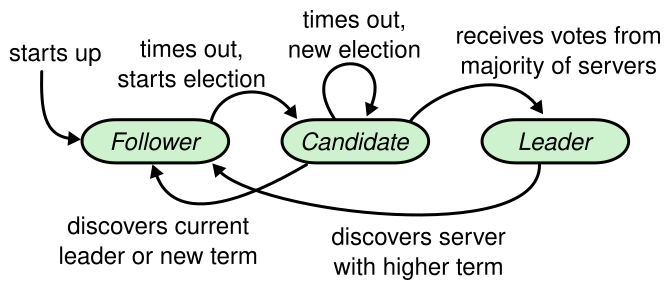
\includegraphics[width=400pt]{images/followercandidateleader.png}
  \caption{High level overview of the different server states and the transitions between them. It is taken from Diego Ongaro's PhD dissertation \cite{raft}.}
  \label{fig:raft-states-transitions}
\end{figure}

\section{Raft Properties} \label{raft-properties}

One of the reasons Raft has become so prevalent is the guarantees it carries about its behavior. Namely, Raft guarantees the following properties: Election Safety, Leader Append-Only, Log Matching, Leader Completeness, State Machine Safety \cite{raft}. They are essential in keeping Raft implementations simple, since developers can easily reason about the system's behavior. They are also formally proven \cite{raft} and can be trusted to always hold.\\

Each property is briefly described as follows:
\begin{itemize}
    \item \textbf{Election Safety}: At any given term, only one server will be acting as the leader. The leader is responsible for advancing the replicated state machine and needs to do so without conflict.
    \item \textbf{Leader Append-Only}: A server, when acting as the leader, can append commands to its internal log but never overwrite or delete previous commands. This is an essential building block for providing the final three properties.
    \item \textbf{Log Matching}: When the logs of two servers contain a command with the same index that was created in the same term, it is guaranteed that all commands up to and including this command are completely identical in their contents.
    \item \textbf{Leader Completeness}: A command that is successfully committed in a term will always be present in the logs of all subsequent leaders.
    \item \textbf{State Machine Safety}: When a server is instructed to apply a command at a certain index to its state machine, it is guaranteed that no other server will apply a different command at the same index to its own state machine.
\end{itemize}

\section{Fault Tolerance in Raft}

As stated before, Raft is particularly appealing because it can continue advancing the replicated state machine in the face of failures, while not sacrificing its strong consistency guarantees. Specifically, any minority of servers can become in some way non-operational without impeding progress. \\

To make this fact apparent, the exact conditions under which the leader election and log replication processes succeed are presented below.

\subsection{Leader Election} \label{leader-election-fault-tolerance}

During an election cycle, a candidate only needs to gather votes from the majority of the cluster before declaring itself the leader for the term and sending heartbeats to all other servers. Notably, it is possible for multiple servers to become candidates and attempt to solicit votes simultaneously, but at most one of them can succeed. This is ensured by restricting each server to vote for only a single candidate in each term. At worst, none the candidates will receive a majority of votes, resulting in a tie. In that case, after an election timeout, they will attempt to get elected for the next term. Note that each server's vote for each term is made durable by persisting it along with the log, enabling it to survive restarts and other failures.\\

\subsection{Log Replication}

During log replication, a command is considered successfully replicated, or committed, once a majority of the cluster has received and stored it. Then, the command will take effect and will be visible to clients.\\

Raft can guarantee that the internal log of any elected leader will contain all commands committed by previous leaders, even without requiring successful replication to all servers. This is implemented by applying an additional rule during leader election; a voter will reject a candidate if the candidate's log is less up to date than its own. Having this guarantee, newly elected leaders can immediately start accepting requests from clients and further advancing the log safely.\\

Further, it is not possible for a leader that was for a time period not operational to later rejoin the cluster and erroneously modify the replicated log. This is implemented via a restriction during log replication. Leaders attempting to replicate commands include their current term in their requests to followers. A leader that has lost its authority in the cluster will use a stale term, prompting other servers to reject its requests and forcing it to become a follower.\\

\subsection{Failure Types}

At this point, the specific types of failures that Raft can handle should be noted; Raft assumes that a failing server is either unable to function or unable to communicate with other servers.\\

A Raft server can be unable to function due to power loss, hardware failure, or other exceptional conditions that interrupt its runtime. Failing servers will be unable to respond to any requests, either from clients or from other servers.\\

A Raft server can become unable to communicate due to failures in the network infrastructure connecting the cluster, resulting in a network partition. Partitioned servers will look identical to failing servers to the rest of the cluster but, importantly, will still seem operational to servers and clients on the same side of the partition. This characteristic of partitions makes them uniquely dangerous for consensus mechanisms due to their potential for causing split-brains. This will be discussed further in subsection \ref{split-brains}.\\

Raft can tolerate both of these cases as long as there is still a majority of operational servers that can communicate. Notably, Raft cannot cope with servers that fail by exhibiting arbitrary or malicious behavior. Such conditions are called Byzantine faults in the literature and there have been efforts to describe a version of Raft that can effectively guard against them \cite{tian2021byzantine,xie2022raft,zhou2021vg,copeland2016tangaroa}. \\

\subsection{Guarding Against the Split-Brain Problem} \label{split-brains}

As mentioned previously, network partitions give rise to the unique problem of split-brains in consensus mechanisms. A cluster of servers enters a split-brain condition when groups of servers are isolated from each other, resulting in the erroneous formation of multiple independent clusters.\\

Raft in its original form can effectively prevent split-brains without modification; the described log replication and leader election processes can only succeed if a majority of the cluster can communicate. If a cluster gets partitioned, there will be at most one majority formed, which can continue advancing the log safely. If the cluster is partitioned in a way that does not allow for any majority to form, the cluster will become unable to fulfill client requests until the partition is resolved.\\

However, Raft is susceptible to split-brains when the cluster supports dynamic reconfigurations, even in the absence of partitions. Dynamic cluster reconfiguration refers to the addition or removal of servers from the cluster without any interruption of service. If multiple servers are added at once, a window of time is created where separate majorities can form \cite{raft}, as demonstrated by Figure \ref{fig:reconfiguration-difficulty}.\\ 

Permitting only a single server addition at a time will eliminate such cases as it can never result in the formation of separate majorities \cite{raft}. More servers can be added once the previous server addition has been acknowledged by the entirety of the cluster. Additionally, Raft provides a solution for "Arbitrary configuration changes using joint consensus" \cite{raft}. Although this solution can allow more than one server to be added at a time, it is complex and not essential for most real-world applications.


\begin{figure}[ht]
  \centering
  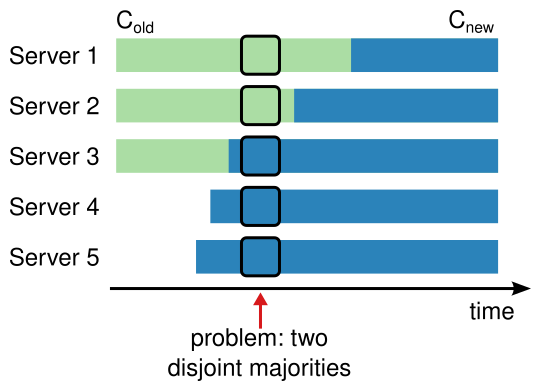
\includegraphics[width=400pt]{images/reconfigurationdifficulty.png}
  \caption{The transition from the old configuration ($C_{old}$) of three servers to the new configuration ($C_{new}$) of five servers happens incrementally and different servers observe it at different times. In this case, there is a period in time where $Server_1$, $Server_2$, and $Server_3$ can form one majority, while $Server_3$, $Server_4$, and $Server_5$ can form another. This figure is taken from Diego Ongaro's PhD dissertation \cite{raft}.}
  \label{fig:reconfiguration-difficulty}
\end{figure}

\section{Scalability concerns in Raft} \label{scalabilirt-raft-multi-raft}

In Raft, larger cluster sizes provide additional fault tolerance, since more servers can become non-operational while still keeping a majority alive. However, a Raft cluster does not improve its performance by using the computational resources of additional servers. At any given point in time, only the leader is performing meaningful work, and other servers act as replicas, ready to take the reigns when the leader fails. In fact, as cluster sizes increase, Raft's processes incur additional overhead, since they require performing broadcast requests to increasingly more servers. 

\subsection{Raft Cluster Sizing}

These performance considerations have generally led to the recommendation that Raft clusters comprise of three, five, or seven servers.\\ 

Three servers is the minimum, as any smaller size provides no fault tolerance. Seven is thought to be a sensible maximum, since it provides enough fault tolerance in real-world use cases while not incurring significant overhead. Clusters of four or six servers, while viable, are not encouraged. These sizes carry the same fault tolerance characteristics of clusters with one less server, incurring needless overhead. To demonstrate this, consider that in clusters of both three and four servers, only a single server can fail, as the majority in the first case requires two, and in the second case three servers. The same is true for clusters of five and six servers; in both cases, at most two servers can fault.\\

\subsection{Increased Scalability with Multi-Raft}

A successful method for achieving higher scalability with Raft has been to segment the replicated state machine into multiple parts, running an independent Raft process for each of them. Incoming client requests are deterministically routed to a single one of these processes, effectively implementing a sharded architecture \cite{solat2024sharding}.
Such a setup has typically been called Multi-Raft and is common in distributed databases that use Raft, such as CockroachDB \cite{cockroachDb-multi-raft}.\\

In the simplest case, all servers in the cluster run one Raft process per state machine. Different servers can then be elected as leaders for each of the independent Raft processes, thus spreading the load. Usually, mechanisms need to be put in place for preventing single servers from becoming the leader for a disproportionately large share of state machines. Additionally, messages generated by each Raft process are usually grouped and sent in batches to other servers, mitigating the increase in message volume caused by the multiple Raft instances.\\

Although the described design spreads the load within a cluster more evenly, it does not enable larger cluster sizes. To achieve that, implementations can restrict the number of servers participating in each of the Raft processes. For example, a cluster of fifteen servers can be used, with each of the processes hosted in overlapping groups of five. In such setups, additional mechanisms need to be put in place for assigning each Raft process to specific servers and for routing client requests to them.\\

\subsection{Utilizing Followers for Reads}

Notably, it is possible for a Raft cluster to utilize follower servers for fulfilling some types of requests, spreading the load somewhat without Multi-Raft.\\

A follower can use its internal log to reply to clients seeking to simply read the current state of the state machine. However, the follower's log may be stale, as the leader might not have replicated a committed command to it yet. Implementations can choose to accept the possibility of staleness, or instruct the follower to first verify that its log is up to date before replying.\\
\chapter{Key-Value Store Implementation}

Having presented the problem of consensus and the constituent parts of Raft, this paper's implementation of a simple consistent distributed database can now be examined. The source code is freely available as a GitHub repository \cite{stoufexis-raft}.

\section{Key-Value Stores}

The distributed database implemented in this paper is a key-value store. Key-value stores are NoSQL databases that store data as pairings of keys and values. A key is thought to uniquely identify a value; thus, the store behaves like an associative array. Usually, key-value stores do not provide built-in methods for managing the schema of values and do not support complex querying.\\

Key-value stores can support a multitude of use-cases, such as metadata storage, dynamic configuration, caching, and the implementation of high-volume aspects of services, such as shopping-carts \cite{aws-kv-stores,consul-kv-stores}. They are quite useful in distributed setups, as their data-sets can be easily partitioned or replicated and can usually support operations on large data volumes with minimal latency \cite{aws-kv-stores}.\\

\section{Overview of the Implementation} \label{impl-overview}

The implemented database runs as a cluster of servers, along with a reverse proxy, which abstracts the server locations. A REST API is exposed to the user, supporting the retrieval, insertion, and update of values associated with keys. Additionally, a lightweight transaction mechanism is provided for atomically modifying the data set. Finally, each request from clients is expected to contain a unique command identifier, enabling the implementation of linearizable semantics. Linearizable semantics are explained in Subsection \ref{linearizable-semantics}.\\

Raft is used to achieve consistency within the cluster. The set of key-value pairs forms a Raft state machine, with the initial state of an empty set. Each request maps to a Raft command, which is replicated and committed before applying. With each application, the state machine transitions and produces a response that is returned to the client. Thus, consensus is always reached for each modification of the data-set, making it fault-tolerant and consistent across the cluster.\\

Specifically, the following REST endpoints are provided:
\begin{enumerate}
    \item \lstinline|GET /store/{COMMAND_ID}/?keys={KEY_1}&keys={KEY_2}&...|: Retrieves the values currently associated with a set of keys. Along with the values, an identifier called the revision id is returned which can be used with endpoint 3.
    \item \lstinline|PUT /store/{COMMAND_ID}/?{KEY_1}={VALUE_1}&{KEY_2}={VALUE_2}&...|: Inserts the given key-value pairs. If a key already exists it is updated with the given value. A key-value pair can be deleted by providing an empty value for the key.
    \item \lstinline|PUT /store/tx/{COMMAND_ID}/{REVISION_ID}/?{KEY_1}={VALUE_1}&{KEY_2}={VALUE_2}&...|: Behaves identically to the previous endpoint, but only takes effect if a set of reference keys have not been modified since they were previously read. The reference keys are validated through the revision id, which must also be given.
\end{enumerate}

Any client may address a request to any of the servers in the Raft cluster, but the response may be a redirection to another server if the reached server is not the leader.\\

It is worth pointing out that, even though the Raft log is persisted to disk, a snapshot of the latest state of the key-value store is always held in memory. This decreases latency, as the state does not need to be rebuilt from the Raft log on each operation. On the flip-side, it restricts the size of the data-set to the size of the available memory of each machine hosting the Raft servers. Since the main goal of key-value store implementation was simplicity and understandability, this bottleneck was not further optimized. In real-world implementations, part of the data-set may be offloaded to disk.

\subsection{Implementing Transactions} \label{implementing-transactions}

The third listed endpoint can be used to implement transactions via simple optimistic locking \cite{kung1981optimistic} using the following process:
\begin{enumerate}
    \item A client reads any set of keys using the first endpoint, retrieving their value along with a revision id which uniquely identifies their current state. The read keys are used as the reference keys.
    \item Then, the client, knowing the current values of the reference keys, attempts to insert any set of key-value pairs via the third endpoint. The operation is rejected if any reference key has been modified by another client since it was read. This is achieved by requiring the client to provide the revision id that was retrieved on the first step.
    \item If the operation is rejected, the new values of the reference keys are returned along with the new revision id. The client then retries its operation by issuing a new request to the third endpoint. This read-and-insert cycle completes once an insert succeeds, in which case the operations were executed atomically.
\end{enumerate}

Since this transaction mechanism can use any set of keys as the reference and any set of keys as the input, it can be used to implement any atomic read-and-insert type of operation. Note that this general design is used in many atomic data structures, such as in the \lstinline|getAndUpdate| method of \lstinline|AtomicReference| in Java \cite{get-and-update}. Usage examples of this feature will be given in Subsection \ref{transactions-scenario}.\\

It is also worth noting that the transaction is completely durable, even if the Raft leader, or any server, fails after any of the steps, the transaction can be continued by the subsequent leaders.\\

\section{Programming Language and Tools} \label{language-tools}

Before delving into the implementation details of the key-value store, the tools that were used, including programming languages, methodologies, libraries, services, and platforms, are presented.

\subsection{Programming Language}

The Scala programming language is a strongly typed, expressive language that runs on the JVM. It powers some of the world's largest distributed systems, including large financial platforms, streaming platforms such as Netflix \cite{netflix}, Disney Streaming \cite{disney-streaming} and Spotify \cite{spotify}, social media platforms such as Twitter \cite{x-twitter}, gaming platforms such as Lichess \cite{lichess}, big data frameworks such as Spark \cite{spark}, and many others.\\

Due to its pervasiveness and utility in the implementation of distributed systems, it was picked as the go-to language for this thesis.

\subsection{Programming Style}

Scala's expressiveness and type system facilitate a popular programming style, known as pure functional programming. This style, popularized by the Haskell programming language, models programs as pure mathematical structures and operates on them via well-defined and safe operations that possess provable properties.\\

Modeling programs as purely mathematical structures allows the concise expression of complex logic with minimal effort, while speeding up the development process, reducing the occurrences of bugs, and aiding in the long-term maintenance of the code \cite{pure-fp-scala}. This style of programming was used throughout the implementation of the key-value store, as it is invaluable for implementing complex concurrent algorithms.

\subsection{Libraries}

\begin{itemize}
    \item \textbf{cats-effect}: The cats-effect library is the gold standard for concurrency within the Scala ecosystem. It provides a lightweight, reliable asynchronous runtime for Scala, along with abstractions and data structures for writing asynchronous and concurrent programs. It was used throughout the project to achieve high throughput while preserving the reliability of the system.
    \item \textbf{fs2}: Fs2 integrates with cats-effect and provides an additional purely functional data structure, called a Stream. A Stream represents a discrete, lazily produced sequence of values which allows complex transformations using sequential or concurrent operations. The fs2 Stream was used to implement all the core parts of the key-value store. 
    \item \textbf{http4s}: Http4s is a standard solution for implementing http servers and clients using cats-effect and fs2 in Scala. It was used both for implementing the user-facing REST API and for server-to-server communication within the Raft cluster.
    \item \textbf{log4cats}: Log4Cats provides tools for purely functional logging within the cats-effect ecosystem of libraries. As there was a need for traceability, logging had to be introduced in the project and this library was the go-to tool.
    \item \textbf{circe}: Circe is a JSON library for Scala. It enables the abstract representation of a JSON document, as well as conversions between Scala data types and JSON. Circe was necessary as JSON was the format of choice for server-to-client as well as server-to-server communications in the key-value store.
    \item \textbf{scodec}: Scodec enables conversions between Scala data types and byte streams. It was used for generating and parsing revision ids.
    \item \textbf{sqlite}: Sqlite is a fully embedded SQL database engine that is used for persisting and retrieving data from local storage using SQL. It is probably the most used database engine in the world \cite{sqlite-most-used} and was used as the backbone for the persistence layer of the key-value store.
    \item \textbf{doobie}: Doobie is a JDBC client that integrates with cats-effect and fs2. It was used to communicate with the Sqlite database.
\end{itemize}

\subsection{Other Tools}

\begin{itemize}
    \item \textbf{Sbt}: Sbt is the build tool of choice for most Scala projects. It was used for organizing, packaging, building, and testing the code-base.
    \item \textbf{Sbt Native Packager}: A plugin for Sbt which enables packaging Scala applications into various formats. The key-value store uses this plugin to package the application into a Docker image.
    \item \textbf{Scalafmt}: Scalafmt is a code formatter for Scala. It was used for enforcing formatting rules over the code-base to keep it easily readable.
    \item \textbf{Vscode}: Vscode is a code editor that supports most modern programming languages. It was the main tool for authoring the code-base.
    \item \textbf{Metals}: Metals is a language server that integrates well with Vscode and Sbt. It has advanced linting capabilities and it was used for continually enforcing that the code-base can successfully compile, as well as for executing Sbt actions through Vscode, such as building and running the code.
    \item \textbf{Docker}: Docker has become the tool of choice for packaging applications into images and running these images in containers within a managed runtime. The key-value store deploys its servers as a group of Docker containers and it takes advantage of Docker's networking features.
    \item \textbf{Docker Compose}: Docker Compose is used for configuring and deploying Docker containers in a cluster, based on a configuration file. The key-value store comes with a configuration for deploying an experimental cluster for testing.
    \item \textbf{Nginx}: Nginx is a web server, but it is also used as a reverse proxy, a load balancer, a mail proxy, and in other configurations. The key-value store, in its experimental setup, uses Nginx as a reverse proxy, to abstract the details of the cluster from clients.
    \item \textbf{Git}: Git is the modern standard for version control in software projects and was used for that purpose over the entire code-base. 
    \item \textbf{GitHub}: GitHub is a platform for hosting Git repositories, publishing documentation, executing CI/CD pipelines, and many more use cases. It was used for hosting and publishing the code-base.
\end{itemize}

\section{Source Code}

As all the necessary foundation has been laid out, the source code of the key-value store implementation can now be examined in detail.

\subsection{Modules}

The project is spread between two modules, which are built separately by Sbt; \lstinline|raft| and \lstinline|kvstore|.\\

The \lstinline|raft| module contains a generic implementation of the Raft consensus algorithm. Users of this module need to provide implementations for a set of defined interfaces, known as traits in Scala, describing the state machine, persistence layer, server-to-server communication, and server-to-client communication.\\

The \lstinline|kvstore| module depends on the \lstinline|raft| module, implementing the key-value store by providing implementations for all required interfaces. It uses Sqlite for persistence and HTTP for server-to-server and server-to-client communication. The Doobie library is used for interacting with Sqlite, while the http4s library is used to define and run the necessary HTTP server and client. It also includes configuration for running a simple cluster, used for testing.

\subsection{Packages}

The source-code is further organized into packages for each of the modules.\\

The \lstinline|raft| module includes the following packages:
\begin{itemize}
    \item \lstinline|com.stoufexis.raft|: This is the root package, containing all other packages and top-level definitions that are required for users of the module.
    \item \lstinline|com.stoufexis.raft.model|: Contains definitions of core data types that are used throughout the implementation.
    \item \lstinline|com.stoufexis.raft.persist|: Defines the two traits that users of the module must implement to enable persistence.
    \item \lstinline|com.stoufexis.raft.rpc|: Contains definitions of data types and functions used for server-to-server and server-to-client communications. Some parts of the implementation are missing, allowing users of the module to plug in any underlying technology.
    \item \lstinline|com.stoufexis.raft.statemachine|: Contains the generic Raft implementation and all its core functions and data types. The definition of the state machine to be replicated and its input and output types are not hard-coded, allowing the user to provide any implementation.
    \item \lstinline|com.stoufexis.raft.typeclass|: Contains definitions of type classes \cite{wadler1989make} used in some generic functions.
\end{itemize}

The \lstinline|kvstore| module includes the following packages:
\begin{itemize}
    \item \lstinline|com.stoufexis.raft.kvstore|: This is the root package, containing all other packages and top-level definitions, including the entry-point for running the key-value store application.
    \item \lstinline|com.stoufexis.raft.kvstore.persist|: Uses Sqlite and Doobie to provide implementations for the traits defined in \lstinline|com.stoufexis.raft.persist|.
    \item \lstinline|com.stoufexis.raft.kvstore.rpc|: Uses http4s to plug in an HTTP-based implementation for the missing parts of \lstinline|com.stoufexis.raft.rpc|.
    \item \lstinline|com.stoufexis.raft.kvstore.statemachine|: Provides the definition of the state machine, implementing the core logic of the key-value store, along with its input and output types. The state machine definition is provided to the \lstinline|raft| module, which replicates it across the cluster.
\end{itemize}

\subsection{Data Types and Functions}

Next, a brief description of the defined functions and data types is provided, per package. Parts of the source code deemed entirely self-explanatory or non-essential for the reader's understanding are left out. For a greater level of detail, the reader is encouraged to also inspect the source code in the GitHub repository \cite{stoufexis-raft}.

\subsubsection{Notes on Notation}

In the following lists, a name containing a period denotes one of the following:
\begin{itemize}
    \item A member of a class, trait, or object. The right side is the name of the member while the left side is the class, trait, or object.
    \item An extension function. The right side is the name of the function, while the left side is the type for which the extension function is defined.
\end{itemize}

Additionally, note the following:
\begin{itemize}
    \item Function parameters, type parameters, and return types are not shown, but may be mentioned when required.
    \item Unless specified otherwise, Stream refers to the Stream data type provided by fs2.
\end{itemize}

\subsubsection{\lstinline|com.stoufexis.raft|}

\begin{itemize}
    \item \lstinline|ExternalNode|: Trait representing a handle to a Raft server within the cluster other than the current one. An instance of this trait for every external server is given by users of the package, allowing them to use any technology for sending commands from one Raft server to another.
    \item \lstinline|ExternalNode.id|: Unique identifier of the external Raft server.
    \item \lstinline|ExternalNode.appendEntries|: Sends an \lstinline|AppendEntries| command to the external Raft server. The response should be returned to the Raft instance running on this server. This implements the sending side of the AppendEntries RPC, described in detail in Chapter 3 of the Raft paper \cite{raft}.
    \item \lstinline|ExternalNode.requestVote|: Sends a \lstinline|RequestVote| command to the external Raft server. The response should be returned to the Raft instance running on this server. This implements the sending side of the RequestVote RPC, described in detail in Chapter 3 of the Raft paper \cite{raft}.
    \item \lstinline|RaftNode|: Trait representing a handle to the Raft process running on the current server. An instance of this trait is given to users of the Raft package, allowing them to use any technology for receiving commands from clients or from other servers.
    \item \lstinline|RaftNode.appendEntries|: Provides an \lstinline|AppendEntries| command, sent by an external Raft server, to the Raft process running on this server. A response is produced which is expected to be routed back to the sender-server. This implements the receiving side of the AppendEntries RPC, described in detail in Chapter 3 of the Raft paper \cite{raft}.
    \item \lstinline|RaftNode.requestVote|: Provides a \lstinline|RequestVote| command, sent by an external Raft server, to the Raft process running on this server. A response is produced which is expected to be routed back to the sender-server. This implements the receiving side of the RequestVote RPC, described in detail in Chapter 3 of the Raft paper \cite{raft}.
    \item \lstinline|RaftNode.clientRequest|: Provides a command from a client to the Raft instance running on this server. If the current server is the leader, it attempts to commit the command by replicating it to a majority of servers. Once committed, the state machine is advanced and a response is returned containing the result of the command, which should be routed back to the sender-client. If the current server is not the leader, the response is a redirection to the leader.
    \item \lstinline|RaftNode.Builder|: A data type, implementing the builder pattern, which is used for configuring the Raft process.
    \item \lstinline|RaftNode.builder|: Creates an object of type \lstinline|Builder|, providing default values and allowing for further configuration. It requires a unique identifier of the current Raft server, the definition of the state machine to be replicated, and instances of the traits implementing the persistence layer.
    \item \lstinline|RaftNode.Builder.withExternals|: Configures the Raft process of the current server by providing handles to the rest of the servers within the cluster.
    \item \lstinline|RaftNode.Builder.withHeartbeatEvery|: Configures the heartbeat interval used by the Raft process.
    \item \lstinline|RaftNode.Builder.withElectionTimeout|: Configures the election timeout range used by the Raft process.
    \item \lstinline|RaftNode.Builder.withAppenderBatchSize|: Configures the batch size used by the leader when attempting to replicate multiple log entries at once.
    \item \lstinline|RaftNode.Builder.build|: Uses the configuration parameters given to the \lstinline|Builder| to create a \lstinline|RaftNode| instance.
\end{itemize}

\subsubsection{\lstinline|com.stoufexis.raft.model|}

\begin{itemize}
    \item \lstinline|Command|: The pairing of a user-defined command type with a command id.
    \item \lstinline|CommandId|: The unique identifier of a command.
    \item \lstinline|Index|: The sequence number of entries in the replicated log.
    \item \lstinline|Index.init|: The index number of the first entry in the replicated log.
    \item \lstinline|Index.uninitiated|: The index number preceding the \lstinline|init| index.
    \item \lstinline|NodeId|: The unique identifier of a Raft server within the cluster.
    \item \lstinline|Role|: An enumeration representing the state of the current server, either Follower, Candidate, or Leader.
    \item \lstinline|Role.init|: The \lstinline|Role| with which each server starts up.
    \item \lstinline|Term|: The Raft term.
    \item \lstinline|Term.init|: The initial Raft term.
    \item \lstinline|Term.uninitiated|: The term preceding the \lstinline|init| term.
\end{itemize}

\subsubsection{\lstinline|com.stoufexis.raft.persist|}

\begin{itemize}
    \item \lstinline|Log|: Trait enabling the persistence of the Raft log to disk. Users of the \lstinline|raft| package are expected to provide concrete implementations of this trait to the Raft process, which allows them to use any persistence technology.
    \item \lstinline|Log.append|: Appends and persists a non-empty sequence of commands to the Raft log, returning the index of the last entry.
    \item \lstinline|Log.commandIdExists|: Checks whether the log contains a command, given a command id.
    \item \lstinline|Log.matches|: Checks whether there exists an entry in the log with the given index and term. If true, all log entries up to the given index are guaranteed to be identical. This is due to the Log Matching property of Raft as described in Section \ref{raft-properties}.
    \item \lstinline|Log.deleteAfter|: Deletes all log entries after the given index.
    \item \lstinline|Log.range|: Returns all log entries between two indexes.
    \item \lstinline|Log.rangeStream|: Returns all log entries between two indexes as an fs2 Stream.
    \item \lstinline|Log.lastTermIndex|: Returns the term and index of the last entry in the log.
    \item \lstinline|Log.term|: Returns the term of the entry with the given index. If the entry does not exist, an error should be raised, but this function is guaranteed by the Raft implementation to only be called with valid indexes.
    \item \lstinline|PersistedState|: Trait enabling the persistence of data, additional to the Raft log, to disk. The only additional data required by Raft is the candidate for which a server voted during each term's leader election. This ensures that a server can never vote twice in a single term.
    \item \lstinline|PersistedState.persist|: Persists the vote for the given term. If no vote has been made, a \lstinline|None| should be given.
    \item \lstinline|PersistedState.readLatest|: Returns the persisted vote for the latest term.
\end{itemize}

\subsubsection{\lstinline|com.stoufexis.raft.rpc|}

\begin{itemize}
    \item \lstinline|AppendEntries|: The message instructing a follower to append a sequence of entries to its internal log.
    \item \lstinline|AppendResponse|: The response sent by a server after it receives an \lstinline|AppendEntries| message from a leader. It signals success when the entries were successfully appended. Additionally, it may signal failure when the leader's log is not consistent with the follower's or it has a stale term.
    \item \lstinline|RequestVote|: The message soliciting a vote from a server.
    \item \lstinline|VoteResponse|: The response sent by a server after it receives a \lstinline|RequestVote| message from a candidate. It signals whether the vote is granted or rejected. Additionally, it may signal failure when the candidate's term is stale.
    \item \lstinline|ClientResponse|: The response returned to a client by a server after attempting to apply a command. It can signal success by returning the current state along with any output produced by the state machine. Additionally, if the server receiving the command is not the leader, it will redirect to the leader, or inform the client that the leader is not known. Finally, it can inform the client that the command was skipped, which happens when its id was not unique. The conditions for skipping a command are further explained in Subsection \ref{linearizable-semantics}.
    \item \lstinline|ClientResponse.knownLeader|: Constructs a \lstinline|ClientResponse| containing the current leader or informing the client that there is no known leader.
    \item \lstinline|IncomingAppend|: Message used to implement the receiving side of an AppendEntries RPC. It pairs an \lstinline|AppendEntries| message along with a handle for providing an \lstinline|AppendResponse|.
    \item \lstinline|IncomingClientRequest|: Message used to implement the fulfillment of \lstinline|ClientRequest|s. It pairs a \lstinline|Command| along with a handle for providing a \lstinline|ClientResponse|.
    \item \lstinline|IncomingVote|: Message used to implement the receiving side of a RequestVote RPC. It pairs a \lstinline|RequestVote| message along with a handle for providing a \lstinline|VoteResponse|.
    \item \lstinline|InputVotes|: Trait used to implement the receiving side of RequestVote RPCs.
    \item \lstinline|InputVotes.incomingVotes|: Provides a Stream of all \lstinline|IncomingVote|s.
    \item \lstinline|InputAppends|: Trait used to implement the receiving side of AppendEntries RPCs.
    \item \lstinline|InputAppends.incomingAppends|: Provides a Stream of all \lstinline|IncomingAppend|s.
    \item \lstinline|InputClients|: Trait used to implement the fulfillment of \lstinline|ClientRequest|s.
    \item \lstinline|InputClients.incomingClientRequests|: Provides a Stream of all \lstinline|IncomingClientRequest|s.
    \item \lstinline|InputSource|: Extends from the \lstinline|InputVotes|, \lstinline|InputAppends|, and \lstinline|InputClients| traits, allowing receiving all three message types.
    \item \lstinline|InputSink|: Trait used to implement the methods of \lstinline|RaftNode|. It receives requests from external servers and clients, routes them to the Raft process, and returns the response for each request back to them.
    \item \lstinline|InputSink.requestVote|: Used to implement the \lstinline|requestVote| method of \lstinline|RaftNode|.
    \item \lstinline|InputSink.appendEntries|: Used to implement the \lstinline|appendEntries| method of \lstinline|RaftNode|.
    \item \lstinline|InputSink.clientRequest|: Used to implement the \lstinline|clientRequest| method of \lstinline|RaftNode|.
    \item \lstinline|Inputs|: Extends from \lstinline|InputSource| and \lstinline|InputSink|, packaging them in one trait for easier usage.
    \item \lstinline|Inputs.apply|: Creates an instance of the \lstinline|Inputs| trait by implementing the receiving and sending side of each message type using 
    \lstinline|RequestQueue|s. Each of the sending methods enqueues an element while each of the receiving methods consumes elements from the queues as a Stream.
    \item \lstinline|RequestQueue|: A special implementation of a purely-functional, concurrent, bounded queue, holding requests. Enqueued elements are ordered in normal FIFO fashion, but they are not removed from the queue immediately when dequeued. Instead, a request is "committed" and removed when the consumer of the queue provides a response for it. This maintains elements in the queue during state transitions, without losing dequeued requests and without blocking the transition until they are processed. If an element is dequeued but its processing is interrupted because of a state transition, e.g. from Leader to Follower, it remains in the queue and is picked up by the Raft process in the next state, as it was not committed.
    \item \lstinline|RequestQueue.consume|: Consumes from the queue by receiving a Stream of uncommitted elements, along with a handle for committing them.
    \item \lstinline|RequestQueue.offer|: Offers an element to the queue and awaits for it to be committed, returning the response. If the queue has reached its bound, the offer will wait until there is room.
    \item \lstinline|RequestQueue.tryOffer|: Offers an element to the queue and awaits for it to be committed, returning the response. If the queue has reached its bound, the offer immediately returns a value of \lstinline|None| instead of waiting.
    \item \lstinline|RequestQueue.apply|: Creates a \lstinline|RequestQueue| with the given bound.
    \item \lstinline|RequestQueue.Unprocessed|: Utility class used to implement the core internal operations of the \lstinline|RequestQueue|.
    \item \lstinline|RequestQueue.Unprocessed.tryOffer|: Internal method used to implement \lstinline|RequestQueue.tryOffer|.
    \item \lstinline|RequestQueue.Unprocessed.offer|: Internal method used to implement \lstinline|RequestQueue.offer|.
    \item \lstinline|RequestQueue.Unprocessed.drop|: Drops an element from the queue after it is committed. It's an internal method used to implement \lstinline|RequestQueue.offer| and \lstinline|RequestQueue.tryOffer|.
    \item \lstinline|RequestQueue.Unprocessed.read|: Internal method used to implement \lstinline|RequestQueue.consume|.
    \item \lstinline|RequestQueue.Unprocessed.apply|: Creates an instance of the \lstinline|Unprocessed| class by initializing its internal state. It allows for the state's concurrent access by wrapping it in a cats-effect \lstinline|Ref|.
    \item \lstinline|RequestQueue.State|: Used to hold the internal state of the \lstinline|RequestQueue|. It contains the index of the last element of the queue, a \lstinline|Map| containing all the currently uncommitted elements, and a Scala \lstinline|Queue| holding handles to fibers that are waiting to enqueue an element.
    \item \lstinline|RequestQueue.State.elemsBetween|: Helper function that returns all uncommitted elements within a range of indexes.
    \item \lstinline|RequestQueue.State.empty|: Constructs an object of \lstinline|RequestQueue.State| with an index of 0, an empty \lstinline|Map| of elements, and an empty Scala \lstinline|Queue| of waiting fibers.
\end{itemize}

\subsubsection{\lstinline|com.stoufexis.raft.statemachine|}

\begin{itemize}
    \item \lstinline|AppenderCfg|: Case class configuring the heartbeat interval and the batch size used when appending entries.
    \item \lstinline|Automaton|: Case class containing the definition of the user-provided state machine.
    \item \lstinline|Automaton.apply|: Transitions the state machine by providing the current state and an input command from a client. The result of the transition is the new state, along with an output message that should be returned to the client.
    \item \lstinline|Behaviors|: Holds a list of processes that are to be run concurrently, implementing the various components of each of the three server states. Each process is modeled as Stream, which runs indefinitely, but may terminate by producing a single value. The produced value is of type \lstinline|NodeInfo| and it triggers the transition of the server to a new state.
    \item \lstinline|Behaviors.raceFirst|: Runs all the processes concurrently, waiting for any of them to terminate and produce a value of type \lstinline|NodeInfo|. When a value is produced, all other process are interrupted and the value is returned.
    \item \lstinline|Behaviors.++|: Appends a sequence of processes to the \lstinline|Behaviors| object.
    \item \lstinline|Behaviors.apply|: Creates a Behaviors object with an initial list of processes.
    \item \lstinline|BufferredPublisher|: Trait that wraps an fs2 Topic object and allows for cleanly interrupting its publish methods via a shutdown procedure.
    \item \lstinline|BufferredPublisher.publish|: Publishes a message to the topic, but allows for interruption during the shutdown procedure. Returns true if the message was published successfully and false otherwise
    \item \lstinline|BufferredPublisher.publishOrThrow|: Same as publish, but raises an error if not successful.
    \item \lstinline|BufferredTopic|: Trait extending from \lstinline|BufferredPublisher| that adds a method for registering subscribers to the topic.
    \item \lstinline|BufferredTopic.newSubscriber|: Creates a subscription to the topic that is interrupted during the shutdown procedure. The subscription is modeled as a handle to a Stream of the topic's messages.
    \item \lstinline|BufferredTopic.apply|: Creates an instance of the \lstinline|BufferredTopic| trait. The instance is wrapped in a cats-effect Resource, which ensures that the shutdown procedure is ran after use. The shutdown procedure interrupts all publishers and all subscribers.
    \item \lstinline|Leader|: An object defining all processes that need to be run concurrently when the server is in the leader state.
    \item \lstinline|Leader.apply|: Returns all the leader processes as a \lstinline|Behaviors| object. It creates two instances of \lstinline|BufferredTopic|, which are used for message passing between the processes. One of the topics contains the indexes of new entries in the log. A new index is published to the topic after new entries are written to the log. The second topic contains the match index for each follower servers. An update is published every time the leader successfully appends entries to a follower. Match indexes are explained further in the description of \lstinline|commitIdxFromMatch|.
    \item \lstinline|Leader.votes|: The process responding to vote requests from candidates. Vote requests for the current term are rejected, since the current server is a leader, meaning it has voted for itself. If a request for a newer term is received, the process produces a value signaling the server to fallback to a follower state with an unknown leader. Requests with a stale term are rejected.
    \item \lstinline|Leader.appends|: The process responding to append requests. If a request for a newer term is received, the process produces a value signaling the current server to transition to a follower state, since another server is the leader. Requests with a stale term are rejected.
    \item \lstinline|Leader.commitIdxFromMatch|: Helper function that calculates the commit index from the match indexes of followers. The match index is a position of a follower's log, which marks the latest entry where the follower's log matches completely with the leader's. Calculating it becomes simpler due to the Log Matching property of Raft; the match index is simply the largest index containing a log entry that matches in its index and in its term with an entry from the leader's log. The commit index is calculated as the largest index that is lesser than or equal to the majority of match indexes. Practically, the commit index marks the latest log entry that is present on the majority of the servers' internal logs \cite{raft}.
    \item \lstinline|Leader.stateMachine|: The process accepting commands from clients. Every command is first appended to the internal log. Then, the index of the new command is pushed to one of the topics, instructing the \lstinline|appender| process to replicate it to all followers. The process also listens to updates of match indexes from the other topic and calculates the new commit index after every update using \lstinline|commitIdxFromMatch|. Every time the commit index is incremented, the command matching that index is considered committed and is applied to the state machine, which returns the new state and an output. The output and the new state are sent as a response to the client who sent the command. Many clients may be concurrently waiting for their command to be applied, with a bound on their number enforced by the \lstinline|RequestQueue| backing the process.
    \item \lstinline|Leader.partitionChecker|: The process constantly checking whether a network partition has happened that isolated the current server from the majority of the cluster. If the \lstinline|appender| process does not produce updates in the match index topic from the majority of the cluster for a time period exceeding the election timeout, a partition is detected. When a partition is detected, the server falls back to a follower state. This process is not mandatory for Raft's safety, as a partitioned leader can never modify the replicated log. However, it is useful for a partitioned leader to quickly become a follower even before the partition is solved, so that any clients can stop attempting to address their commands to it.
    \item \lstinline|Leader.appender|: The process tasked with replicating log entries to followers. Each time the \lstinline|stateMachine| process appends an entry to the log, it also publishes the index of the entry to a topic. This process reads from the topic and attempts to replicate the command matching the index to all followers. Each time a command is successfully replicated to a follower, an update is produced to the match index topic. Additionally, if there are no new commands for the duration of a heartbeat interval, the process sends heartbeat requests to each follower. Heartbeat requests are identical to normal replication requests, but contain no entries to be replicated. A successful heartbeat request results in the process re-sending the current match index of the follower to the topic, signaling that it was reachable, but no new entries were replicated.
    \item \lstinline|Candidate|: An object defining all processes that need to be run concurrently when the server is in the candidate state.
    \item \lstinline|Candidate.apply|: Returns all the candidate processes as a \lstinline|Behaviors| object.
    \item \lstinline|Candidate.appends|: The process responding to append requests. If a valid request is received, the process produces a value signaling the current server to transition to a follower state, since another server has become the leader. Requests with a stale term are rejected.
    \item \lstinline|Candidate.inVotes|: The process responding to vote requests from other candidates. Vote requests for the current term are rejected, since the current server is a candidate, meaning it has voted for itself. If a request for a newer term is received, the process produces a value signaling the server to fallback to a follower state with an unknown leader. Requests with a stale term are rejected.
    \item \lstinline|Candidate.solicitVotes|: The process sending vote requests to the rest of the cluster, attempting to win the election. If a majority votes is gathered, the process produces a value signaling the server to transition to a leader state. Note that the candidate always implicitly votes for itself.
    \item \lstinline|Follower|: An object defining all processes that need to be run concurrently when the server is in the follower state.
    \item \lstinline|Follower.apply|: Returns all the follower processes as a \lstinline|Behaviors| object.
    \item \lstinline|Follower.isUpToDate|: Helper function checking if a candidate's log is at least as up-to-date as the current server's log. This implements the additional election rule described in Subsection \ref{leader-election-fault-tolerance}.
    \item \lstinline|Follower.votes|: The process responding to vote requests from candidates. If the follower has already voted for this term, all requests for the term are rejected, otherwise, the first one wins. A request containing a new term causes the current vote, if one exists, to be dropped. Requests with a stale term are rejected.
    \item \lstinline|Follower.appends|: The process responding to append requests. Each time the leader sends an append request, it is validated and appended to the follower's internal log. During validation, the \lstinline|prevLogTerm| and \lstinline|prevLogIndex| attributes are extracted from the request. These two match the index and term of the entry in the leaders log right before the entries in the request. The follower looks up if there is any entry in its own log matching these two. If successful, every entry up to and including the entry matching the \lstinline|prevLogIndex| are identical between the leader and the follower, due to the Log Matching property. The validation then succeeds and the follower adds the entries to its log, right after the position indicated by \lstinline|prevLogIndex|, replacing any conflicting entries. If the validation fails, the follower rejects the request, informing the leader that the logs up to the provided index are inconsistent. The leader then keeps retrying by sending entries, each time starting at an older index, until a consistent point is found. Requests with a stale term are rejected.
    \item \lstinline|Cluster|: A case class containing the unique id of the current server, as well as handles to all other servers in the cluster.
    \item \lstinline|Cluster.allNodes|: The identifiers of all servers in the cluster.
    \item \lstinline|Cluster.otherNodeIds|: The identifiers of all servers in the cluster, excluding the current one.
    \item \lstinline|Cluster.otherNodesSize|: The number of servers in the cluster, excluding the current one.
    \item \lstinline|Cluster.majorityCnt|: How many servers constitute a majority in the current cluster.
    \item \lstinline|Cluster.isMajority|: Function that checks if the provided set of server ids form a majority. The function excludes any server ids that are unknown and then counts the remaining ones.
    \item \lstinline|Deps|: A case class aggregating common parameters of functions within the package.
    \item \lstinline|ElectionTimeout|: A utility for retrieving an election timeout interval.
    \item \lstinline|ElectionTimeout.nextElectionTimeout|: Picks a random election timeout interval from a range.
    \item \lstinline|ElectionTimeout.fromRange|: Creates an \lstinline|ElectionTimeout| object by providing a range of time intervals.
    \item \lstinline|NamedLogger|: Utility for creating a logger with a readable name.
    \item \lstinline|NamedLogger.fromState|: Creates a logger with a name derived from the server's current state.
    \item \lstinline|NodeInfo|: Case class containing core information about a server's state; the current \lstinline|Role|, \lstinline|Term|, and the leader of the cluster, if it is known.
    \item \lstinline|NodeInfo.toFollower|: Overloaded method returning a new \lstinline|NodeInfo| based on the current one, switching the role to follower with a known leader. A new term can optionally be provided.
    \item \lstinline|NodeInfo.toFollowerUnknownLeader|: Overloaded method returning a new \lstinline|NodeInfo| based on the current one, switching the role to follower with an unknown leader. A new term can optionally be provided.
    \item \lstinline|NodeInfo.toVotedFollower|: Method returning a new \lstinline|NodeInfo| based on the current one, switching the role to follower with an unknown leader but with a registered vote for the current term.
    \item \lstinline|NodeInfo.toCandidateNextTerm|: Method returning a new \lstinline|NodeInfo| based on the current one, switching the role to candidate for the next term.
    \item \lstinline|NodeInfo.toLeader|: Method returning a new \lstinline|NodeInfo| based on the current one, switching the role to leader for the current term.
    \item \lstinline|NodeInfo.isNew|: Method checking if the provided term is newer than the current one.
    \item \lstinline|NodeInfo.isNotNew|: Negation of \lstinline|isNew|.
    \item \lstinline|NodeInfo.isExpired|: Method checking if the provided term is stale.
    \item \lstinline|NodeInfo.isCurrent|: Method checking if the provided term is the current term.
    \item \lstinline|NodeInfo.isLeader|: Method checking if the provided id corresponds to the known leader.
    \item \lstinline|NodeInfo.isCurrentLeader|: Method checking if the provided id corresponds to the known leader and the provided term is the current one.
    \item \lstinline|NodeInfo.isVotee|: Method checking if the provided id corresponds to the candidate that has the current server's vote for the current term.
    \item \lstinline|NodeInfo.isCurrentVotee|: Method checking if the provided id corresponds to the candidate that has this server's vote for the current term and that the provided term is the current one.
    \item \lstinline|NodeInfo.hasVoted|: Method checking if the current server is acting as a follower and has voted for a server.
    \item \lstinline|NodeInfo.votedFor|: Method returning the candidate that this server has voted for in the current term, if it is acting as a follower. If the current server is not a follower or it has not voted, a \lstinline|None| value is returned.
    \item \lstinline|StateMachine|: Entry point for running the internal Raft process.
    \item \lstinline|StateMachine.runLoop|: Runs the Raft process. First, it reads the persisted vote from the server's local storage, if there is one. This ensures that no votes are lost if this server had failed before and is now restarting. Then, it assumes the role of follower and runs the follower's processes by calling the \lstinline|raceFirst| function of the follower's \lstinline|Behaviors| object. It then awaits the termination of \lstinline|raceFirst|, which produces a value, informing the run loop of the next state it should transition to. The run loop constructs the \lstinline|Behaviors| object corresponding to the new state, and runs \lstinline|raceFirst| again. The server's vote is persisted between each transition, if one was made for the term. The loop runs indefinitely. Note that the function is non-tail recursive, which is made safe by cats-effect, as it provides stack-safe monadic recursion \cite{freeman2015stack}.
    \item \lstinline|WaitingClient|: Provides operations on a queue of clients waiting for their commands to be committed and a response to be returned. These operations are used to implement \lstinline|Leader.stateMachine|.
    \item \lstinline|WaitingClient.enqueue|: Adds a waiting client to the queue. A waiting client is modeled as the index of the command that the client sent, as well as a handle to provide a response.
    \item \lstinline|WaitingClient.fulfill|: Provided the current commit index and the current state of the state machine, it applies all commands from clients up to the commit index and returns a response to each of them. It returns the resulting state of the state machine along with any remaining clients that did not get a response, as their commands' indexes were greater than the commit index.
    \item \lstinline|ResettableTimeout|: Data type used to implement \lstinline|resettableTimeoutAccumulate|, modeling the three types of supported signals.
    \item \lstinline|ResettableTimeout.outputPure|: Creates an instance of \lstinline|ResettableTimeout| signaling the emission of a value with no side effects.
    \item \lstinline|Stream.resettableTimeoutAccumulate|: A function continually pulling from a Stream and applying a stateful transformation that can be interrupted after a timeout. The function returns a new Stream that produces only a single value, or gets interrupted after a timeout. The caller of this function has to provide an initial state, a timeout duration, an effect to be executed upon a timeout, and a function modeling the stateful transformation. The output of the function is of type \lstinline|ResettableTimeout|, allowing it to signal the reset of the timeout, the skipping of a value, or the output of a value.
    \item \lstinline|Stream.increasing|: Transforms a Stream of numeric elements by only keeping elements that were greater than any preceding ones.
    \item \lstinline|Stream.dropping|: Applies back-pressure to a Stream by internally buffering a set amount of elements. If new elements arrive when the buffer is full, it makes space by dropping old elements. A new Stream is returned, which reads from the internal buffer, emptying it. This ensures that a slow consumer of a Stream will not have to catch up by reading a large amount of enqueued elements. Rather, it will only have to read up to a set amount.
    \item \lstinline|Stream.repeatLast|: Returns a Stream that produces elements pulled from the provided stream, but repeats the last produced element after a period of inactivity.
    \item \lstinline|Stream.mergeEither|: Concurrently merges two Streams by returning a new Stream. The new Stream produces values of the first Stream wrapped in \lstinline|Either.Left| and values from the second Stream wrapped in \lstinline|Either.Right|.
    \item \lstinline|raceFirst|: Overloaded function concurrently pulling from a list of Streams. When one of the Streams produces a value, all streams are interrupted and the value is returned.
    \item \lstinline|raceFirstOrError|: Same as \lstinline|raceFirst| but raises an error if all Streams terminate without producing a value.
    \item \lstinline|AppendEntries.termExpired|: Responds to an \lstinline|AppendEntries| request, rejecting it and informing the requester that its term is stale.
    \item \lstinline|AppendEntries.duplicateLeaders|: Responds to an \lstinline|AppendEntries| request, informing the requester that duplicate leaders have been detected for a term. Then, it raises an error. Duplicate leaders for a term can never be created by Raft, so this is an unrecoverable error, indicating a bug in the implementation.
    \item \lstinline|AppendEntries.accepted|: Responds to an \lstinline|AppendEntries| request, informing that it has been accepted.
    \item \lstinline|AppendEntries.inconsistent|: Responds to an \lstinline|AppendEntries| request, rejecting it and informing the requester that the its log is inconsistent with the current server's.
    \item \lstinline|RequestVote.termExpired|: Responds to a \lstinline|RequestVote| request, rejecting it and informing the requester that its term is stale.
    \item \lstinline|RequestVote.reject|: Responds to a \lstinline|RequestVote| request, denying to vote for the requester.
    \item \lstinline|RequestVote.grant|: Responds to a \lstinline|RequestVote| request, granting the vote to the requester.
    \item \lstinline|Stream.respondWithLeader|: Responds to a command from a client, informing that the current server is not the leader and returning the actual leader's id, if it is known.
\end{itemize}

\subsubsection{\lstinline|com.stoufexis.raft.typeclass|}

\begin{itemize}
    \item \lstinline|Empty|: Type class providing an empty value associated with a type.
    \item \lstinline|Empty.empty|: The empty value associated with a type.
    \item \lstinline|Empty.const|: Creates an instance of \lstinline|Empty| that always returns the given value when \lstinline|empty| is called.
    \item \lstinline|Empty.derived|: Automatically creates an instance of \lstinline|Empty| for case classes containing elements that already have \lstinline|Empty| instances defined.
    \item \lstinline|Empty.getAll|: Gathers the \lstinline|Empty| instances of all types contained in a case class and returns them as a \lstinline|Tuple|.
    \item \lstinline|IntLike|: Type class providing numeric operations for any type that resembles an integer.
    \item \lstinline|IntLike.add|: Enables adding a value of type \lstinline|Int| to values of a type implementing \lstinline|IntLike|.
    \item \lstinline|IntLike.toLong|: Enables converting values of a type implementing \lstinline|IntLike| to \lstinline|Long|.
\end{itemize}

\subsubsection{\lstinline|com.stoufexis.raft.kvstore|}

\begin{itemize}
    \item \lstinline|KvStoreConfig|: Case class aggregating all configuration parameters for the key-value store implementation.
    \item \lstinline|KvStoreConfig.loadFromEnv|: Creates an instance of \lstinline|KvStoreConfig| by loading all configuration parameters from environment variables.
    \item \lstinline|Main|: Contains the entry-point for the key-value store application.
    \item \lstinline|Main.raftNode|: Starts up the Raft process and returns a handle of type \lstinline|RaftNode|.
    \item \lstinline|Main.server|: Runs the HTTP server handling all server-to-server and server-to-client communications.
    \item \lstinline|Main.run|: The entry-point for the application. Starts up the Raft process and the HTTP server.
\end{itemize}

\subsubsection{\lstinline|com.stoufexis.raft.kvstore.persist|}

\begin{itemize}
    \item \lstinline|SqlitePersistence|: Contains implementations for the two traits comprising the persistence layer of Raft: \lstinline|Log| and \lstinline|PersistedState|.
    \item \lstinline|SqlitePersistence.apply|: Creates an instance for \lstinline|Log| and \lstinline|PersistedState| by delegating to an embedded Sqlite database. The database schema is detailed in Subsection \ref{sqlite-schema}.
\end{itemize}

\subsubsection{\lstinline|com.stoufexis.raft.kvstore.rpc|}

\begin{itemize}
    \item \lstinline|Routes|: Contains the definitions of HTTP endpoints used for server-to-server and server-to-client communications.
    \item \lstinline|Routes.apply|: Creates and returns an object describing all HTTP endpoints. The endpoints used by clients are described in the introduction of Section \ref{impl-overview}, while the endpoints used by servers are described in Subsection \ref{rpc-endpoints}.
    \item \lstinline|RpcClient|: Contains the implementation of the \lstinline|ExternalNode| trait for the key-value store.
    \item \lstinline|RpcClient.apply|: Uses an HTTP client to implement \lstinline|ExternalNode|. Each request is retried indefinitely in cases of failure; requests to a server in the cluster that has become non-operational will be re-sent until it becomes operational again and replies, or until the retry loop is interrupted externally.
\end{itemize}

\subsubsection{\lstinline|com.stoufexis.raft.kvstore.statemachine|}

\begin{itemize}
    \item \lstinline|KvCommand|: Data type modeling the three commands supported by the key-value store, described in detail in the introduction of Section \ref{impl-overview}. A client can read, insert, update, or delete the values of a set of keys in a standalone operation or paired atomically with a read.
    \item \lstinline|KvResponse|: Data type modeling the responses produced by the key-value store state machine. Both possible responses signal success, but one carries values associated with keys and a \lstinline|RevisionId|, while the other one has no payload.
    \item \lstinline|KvState|: Data type modeling the state of the key-value store state machine. It keeps track of all key-value pairs in the store along with a revision, indicating when each was last modified. Additionally, it manages the global revision, which is modeled as a \lstinline|Long|. Note that the revision is incremented after each update to the store, and there currently is no mechanism to handle overflows. This means that after 9,223,372,036,854,775,807 modifications, the store will assume undefined behavior. Assuming an exaggerated rate of 100,000 operations a second, the revision will overflow after around 300,000 years of operation, meaning there is no immediate need for concern. Of course, the implementation can also be modified to handle overflows gracefully.
    \item \lstinline|KvState.setAll|: Returns a new \lstinline|KvState| object that modifies the current state by applying a \lstinline|Map| containing key-value pairs. The \lstinline|Map| may contain values for new keys, new values for existing keys, or indicate the deletion of a key, by pairing the key with a \lstinline|None| value. The new state contains an incremented global revision and any keys modified or added are assigned this id.
    \item \lstinline|KvState.revisionMatches|: Checks if the given \lstinline|RevisionId| matches with the current state. If there is a match, then no modifications have been made since a previous read. This is the step confirming that a modification is being made atomically with a read.
    \item \lstinline|KvState.getAll|: Provided a set of keys, returns all the matching key-value pairs along with their revisions.
    \item \lstinline|KvState.valuesForKeys|: Provided a set of keys, calls \lstinline|getAll| and creates an instance of \lstinline|KvResponse| containing the returned key-value pairs and a \lstinline|RevisionId| object.
    \item \lstinline|RevisionId|: Models a set of keys paired with revisions, specifying the last revision on which each key was modified. This is used to implement transactions and is serialized to a Base64 string when sent to clients.
    \item \lstinline|StateMachine|: Contains the core logic of the key-value store state machine.
    \item \lstinline|StateMachine.apply|: Function describing the state machine used by the key-value store. It receives commands, applies them to an instance of \lstinline|KvState|, and returns a response along with a new instance of \lstinline|KvState|. This is provided to the Raft process and is iteratively called with new commands and the updated \lstinline|KvState|s.
\end{itemize}

\subsection{Embedded Database Schema} \label{sqlite-schema}

As stated above, the persistence layer for the key-value store is implemented using Sqlite. Two tables are used to implement the \lstinline|com.stoufexis.raft.persist.Log| and \lstinline|com.stoufexis.raft.persist.PersistedState| traits, with all operations translated to series of \lstinline|SELECT|, \lstinline|INSERT|, and \lstinline|DELETE| statements.

\subsubsection{Log Table}

The Raft log is stored in a dedicated table. The schema is shown in Figure \ref{fig:sqlite-schema}. Each row stores the term as an \lstinline|INTEGER|, the command id as \lstinline|TEXT|, and the log entry as \lstinline|TEXT|. The log entry is converted to JSON before inserting. Additionally, all Sqlite tables, unless specified otherwise, contain a unique, auto-incrementing integer column called the ROWID, which acts as the primary key \cite{sqlite-rowid}. This ROWID is used as the Raft index for the log. A unique index on the command id is also created to support efficient look-ups.\\

\subsubsection{PersistedState Table}

The server's vote for each term is stored in an additional table, shown in Figure \ref{fig:sqlite-schema}. The term is stored as an \lstinline|INTEGER| and is used as the primary key, making it not null. The server's vote for each term is stored in a \lstinline|TEXT| column, which contains the candidate's identifier. The vote is nullable, since there are terms for which the server does not cast any vote.

\begin{figure}[ht]
  \centering
  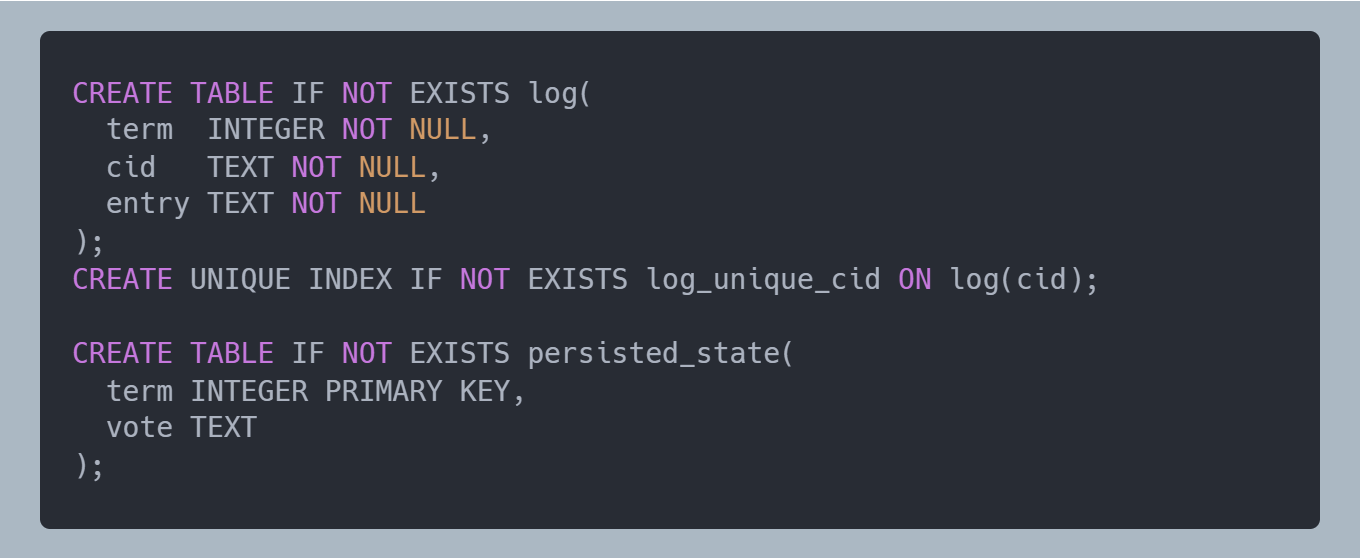
\includegraphics[width=400pt]{images/sqlite-schema.png}
  \caption{Schema used to implement Raft's persistence layer.}
  \label{fig:sqlite-schema}
\end{figure}

\subsection{REST API Specification for Server-To-Server Communication} \label{rpc-endpoints}

In addition to the client-facing endpoints described in the introduction of Section \ref{impl-overview}, there are two more defined for message-passing between servers.
%%begin novalidate
\begin{enumerate}
    \item \lstinline|PUT /raft/append_entries|: Is called by external servers to send an \lstinline|AppendEntries| request. An HTTP body containing the request encoded as JSON is expected. 
    \item \lstinline|PUT /raft/request_vote|: Is called by external servers to send a \lstinline|RequestVote| request. An HTTP body containing the request encoded as JSON is expected.
\end{enumerate}
%%end novalidate

\section{Testing Cluster Deployment} \label{testing-cluster-deployment}

The key-value store module is packaged into a Docker image using Sbt. The configuration for achieving this can be found in the \lstinline|build.sbt| file at the root of the project's source code.\\

Additionally, the key-value store comes with a configuration for deploying a cluster of servers in Docker containers, along with an Nginx reverse proxy, using Docker Compose. This setup is used for experimenting and testing the system, but is not adequate for a production setting. Its main flaw is the single Nginx instance, which is a single point of failure and potentially a bottleneck. These flaws are not relevant though, since this setup's only purpose is to verify the store's behavior and would not be used in a production deployment.\\

The Docker Compose configuration is shown in Figures \ref{fig:kvstore-docker-compose-A} and \ref{fig:kvstore-docker-compose-B}. Each part is described in detail, since it provides a complete and succinct overview of how a Raft cluster is typically structured.

\begin{figure}[ht]
  \centering
  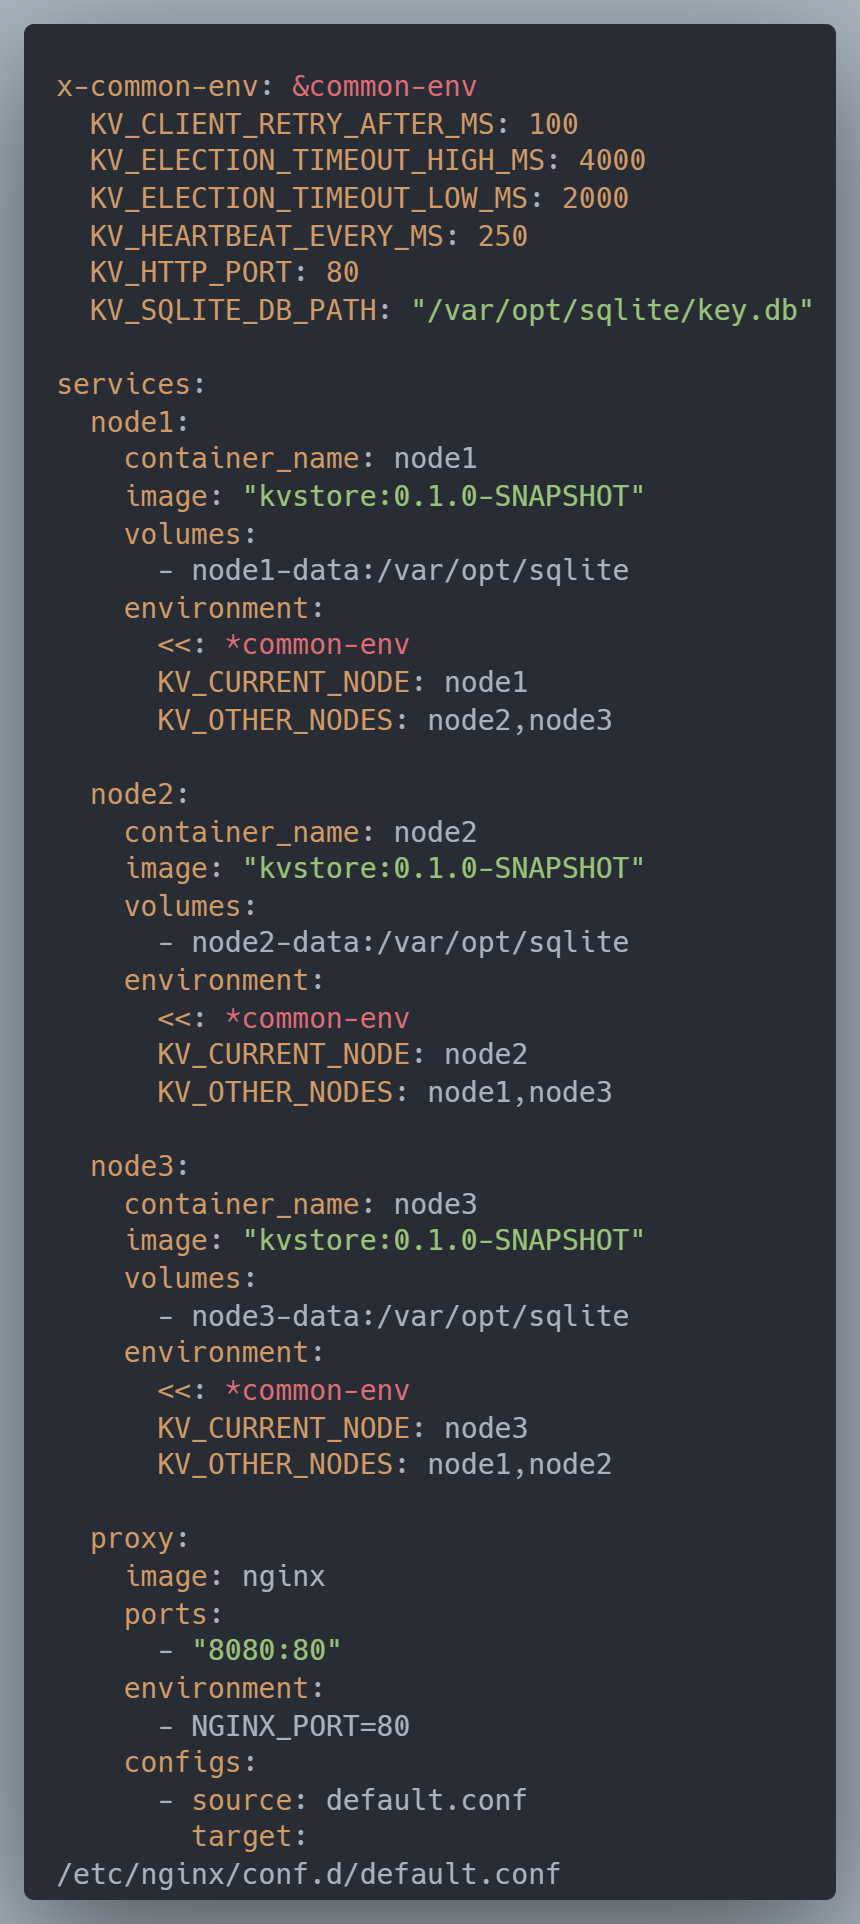
\includegraphics[width=265pt]{images/kvstore-docker-compose-A.png}
  \caption{First part of the Docker Compose configuration. It shows the configuration for deploying three key-value store servers, along with an Nginx proxy. The proxy configuration along with the definition of the required data volumes are shown in Figure \ref{fig:kvstore-docker-compose-B}.}
  \label{fig:kvstore-docker-compose-A}
\end{figure}

\begin{figure}[ht]
  \centering
  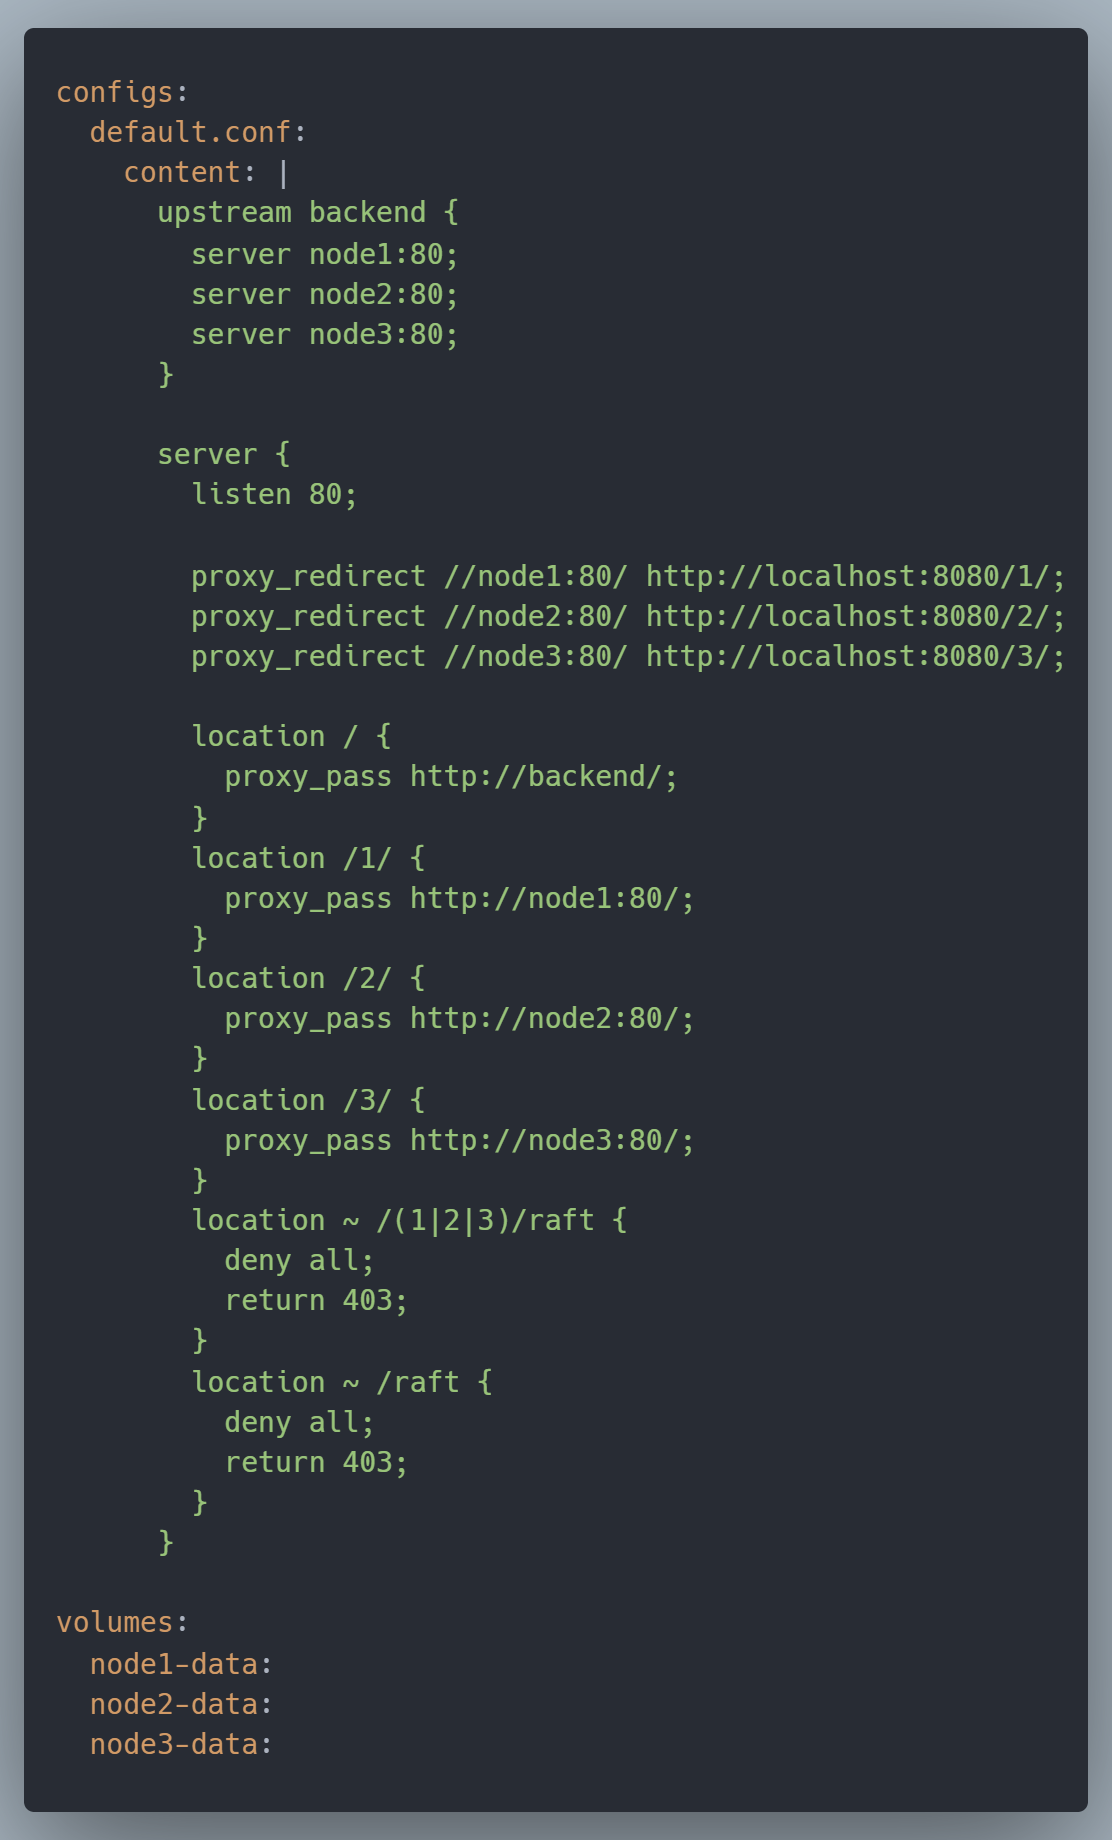
\includegraphics[width=350pt]{images/kvstore-docker-compose-B.png}
  \caption{Continuation of Figure \ref{fig:kvstore-docker-compose-A}, showing the configuration for the Nginx reverse proxy along with the definition of the required data volumes.}
  \label{fig:kvstore-docker-compose-B}
\end{figure}

\subsection{Key-Value Store Server Configuration}

As shown in Figure \ref{fig:kvstore-docker-compose-A}, three key-value store servers are deployed. All of them use identical values for some configuration parameters, which are placed in the \lstinline|x-common-env| object and injected into the environment sections of all servers:
\begin{itemize}
  \item \lstinline{KV_CLIENT_RETRY_AFTER_MS}: How long to wait between retries when a server-to-server communication fails. It is set to 100 milliseconds.
  \item \lstinline{KV_ELECTION_TIMEOUT_HIGH_MS}: The upper bound for the election timeout range. It is set to 4000 milliseconds, or 4 seconds.
  \item \lstinline{KV_ELECTION_TIMEOUT_LOW_MS}: The lower bound for the election timeout range. It is set to 2000 milliseconds, or 2 seconds.
  \item \lstinline{KV_HEARTBEAT_EVERY_MS}: The heartbeat interval. It is set to 250 milliseconds.
  \item \lstinline{KV_HTTP_PORT}: The port that the HTTP server listens to for all communications. It is set to the default HTTP port, 80.
  \item \lstinline{KV_SQLITE_DB_PATH}: The location in each container's file system that Sqlite places its database file. It is set to \lstinline{/var/opt/sqlite/key.db}.
\end{itemize}

Furthermore, all servers are configured with their own unique identifier, under \lstinline{KV_CURRENT_NODE}, and with the identifiers of the other servers, under \lstinline{KV_OTHER_NODES}. The identifiers match the container names of each server, which ultimately map to their hostnames within the cluster, as they are part of the same Docker network. As a result, knowing a server's identifier is enough to send an HTTP request to it from within the Docker network simply by using the identifier as the target hostname.

\subsection{Proxy Configuration and Redirects}

Although the server containers would be adequate for implementing the distributed key-value store, there are several problems and inconveniences that need to be addressed:
\begin{enumerate}
    \item The servers belong in a single docker network without exposing any ports, meaning that they are not reachable from the outside.
    \item If the servers were to expose their ports directly to the outside, clients would need to implement some sort of discovery procedure for learning their locations. This leaks implementation details and forces the cluster to remain as static as possible to not force clients to go through additional discovery procedures.
    \item Each server exposes its entire set of endpoints under the same port, including the ones that should not be accessed by clients. This allows clients to perform arbitrary actions within the Raft cluster, since there is no authorization mechanism in place.
\end{enumerate}

Nginx is used as a reverse proxy to address all these problems, and its configuration is shown in Figure \ref{fig:kvstore-docker-compose-B}. \\ 

To address the first two problems, the Nginx container exposes a port, which clients can use for interacting with the key-value store. A client can address the cluster as a whole, allowing Nginx to route the request to one of the servers. This is achieved by grouping all the servers with the \lstinline{backend} upstream, which is reachable via the \lstinline{/} path. The discovery process is simplified, since a client can address the cluster as a whole, and it will be redirected to the proper recipient for its request. Additionally, after a client learns about a specific server, it can address it by prefixing an endpoint with the server's number. \\

The Nginx configuration also disallows any access to endpoints prefixed with \lstinline{raft}. These must only be called by other servers, as they are used for appending entries and requesting votes.\\

Note that this configuration assumes a static setup, where servers are not added or removed dynamically. The shape of the cluster can only change through an interruption of service, where all the servers and the proxy are shut down, reconfigured, and then redeployed.

\subsection{Data Volumes}

Each server is configured with a unique Docker volume, used to persist the Sqlite database in the file system. The volumes' configuration is shown in Figure \ref{fig:kvstore-docker-compose-B}, while their usage is shown in Figure \ref{fig:kvstore-docker-compose-A}. Having these volumes means that containers can be freely shut down and restarted without data loss.

\section{Linearizable Semantics} \label{linearizable-semantics}

As mentioned several times before, Raft makes several design choices to support linearizable semantics. This is explained in detail in Chapter 6 of the original Raft paper \cite{raft}. The key-value store implementation also supports linearizable semantics, but in a simplified fashion.

\subsection{Requirements of Linearizable Semantics}

Linearizable semantics are important for making a distributed system easy to reason about. The authors of the Raft paper describe them as follows: "In linearizability, each operation appears to execute instantaneously, exactly once, at some
point between its invocation and its response."\cite{raft}.\\

To implement them, there are two requirements that the Raft implementation must fulfill \cite{raft}: 
\begin{enumerate}
    \item Any operation, read or write, must be executed based on an up-to-date view of the system's state and return a response only once committed.
    \item Operations must get executed exactly once.
\end{enumerate}

\subsection{Implementation of Linearizable Semantics in the Key-Value Store}

To address the first requirement, all commands are routed to the leader, which is the single authority on the current state of the system. Before returning a response, the leader appends the command to its log and attempts to commit it by replicating it to the rest of the cluster. Importantly, this also encompasses commands which simply read from the state; the Raft implementation appends them in the log like any other command before replying. This ensures that the leader is still the authority on the current state when responding, as it successfully manages to commit an entry.\\

The second requirement is fulfilled by expecting clients to include a unique identifier along with their commands. If a command is somehow received twice by the system, due to the client retrying, a duplication caused by the network, or another reason, it is identified as a duplicate using its id and it is rejected. The command ids are also stored in the log, so they are completely durable. Note that this implementation is far simpler than how it is described in the original Raft paper, which also stores the response and returns it instead of rejecting the duplicate command, using a session mechanism. Although this would be a more complete solution, it adds a lot of implementation overhead and it was deemed not worthwhile for the key-value store.

\chapter{Results}

This chapter aims to show the key-value store implementation in action, in various scenarios, using the cluster setup detailed in Section \ref{testing-cluster-deployment}. Each scenario will present an initial state of the store and will describe some input, showing the system's reaction through its logs and responses. Then, the store's resulting state will be detailed, showing that it reaches consensus properly, following the previous chapters' descriptions.\\

Note that this list of scenarios is by no means complete, as the combinations of possible states and inputs are near infinite. It should, however, demonstrate the store's capabilities under common conditions as well as several edge cases.

\section{Methodology} \label{results-methodology-intro}

\subsection{Tools}

The following tools were used in this chapter, in addition to those laid out in Section \ref{language-tools}:
\begin{enumerate}
    \item \textbf{curl}: Curl is a command line tool that is often used for issuing HTTP requests from the terminal. It was used to send simple one-shot requests to the store throughout this chapter.
    \item \textbf{scala-cli}: Scala-cli is a utility that allows users to define and run scripts using the Scala language. It was used to script complex and concurrent series of requests.
\end{enumerate}

\subsection{How to Read the Figures}

In addition to the description of the system's state and output, each scenario will display the servers' log files in figures, as presented by the \lstinline|docker compose logs| command. The logs will be abbreviated when necessary, with a placeholder of three dots "\lstinline|...|" used in place of a removed section of text. Alongside the servers' logs, any commands used to interact with the cluster will also be shown in figures.\\

All the presented figures will contain numbered markers inside parentheses. These markers will be referenced to explain the series of events that took place in each scenario. Each marker groups a series of lines in the shown figures, spanning from the line the marker is placed on up to the line right before the next marker. The last marker in each figure spans until the end. A marker with the same number may be used across multiple figures in each scenario, associating an input with the system's reaction. For example, it may show that a log message produced by the cluster is caused by a specific request executed via the terminal.\\

\section{Scenarios}

\subsection{Leader Election After Startup}

This scenario showcases the cluster's behavior after the very first time it starts up.

\subsubsection{Initial State}

The cluster is shut down; there are no servers or proxies running.

\subsubsection{Input}

The cluster is started using the \lstinline|docker compose up| CLI command via the terminal, shown in Figure \ref{fig:scenario-1}.

\begin{figure}[ht]
\centering
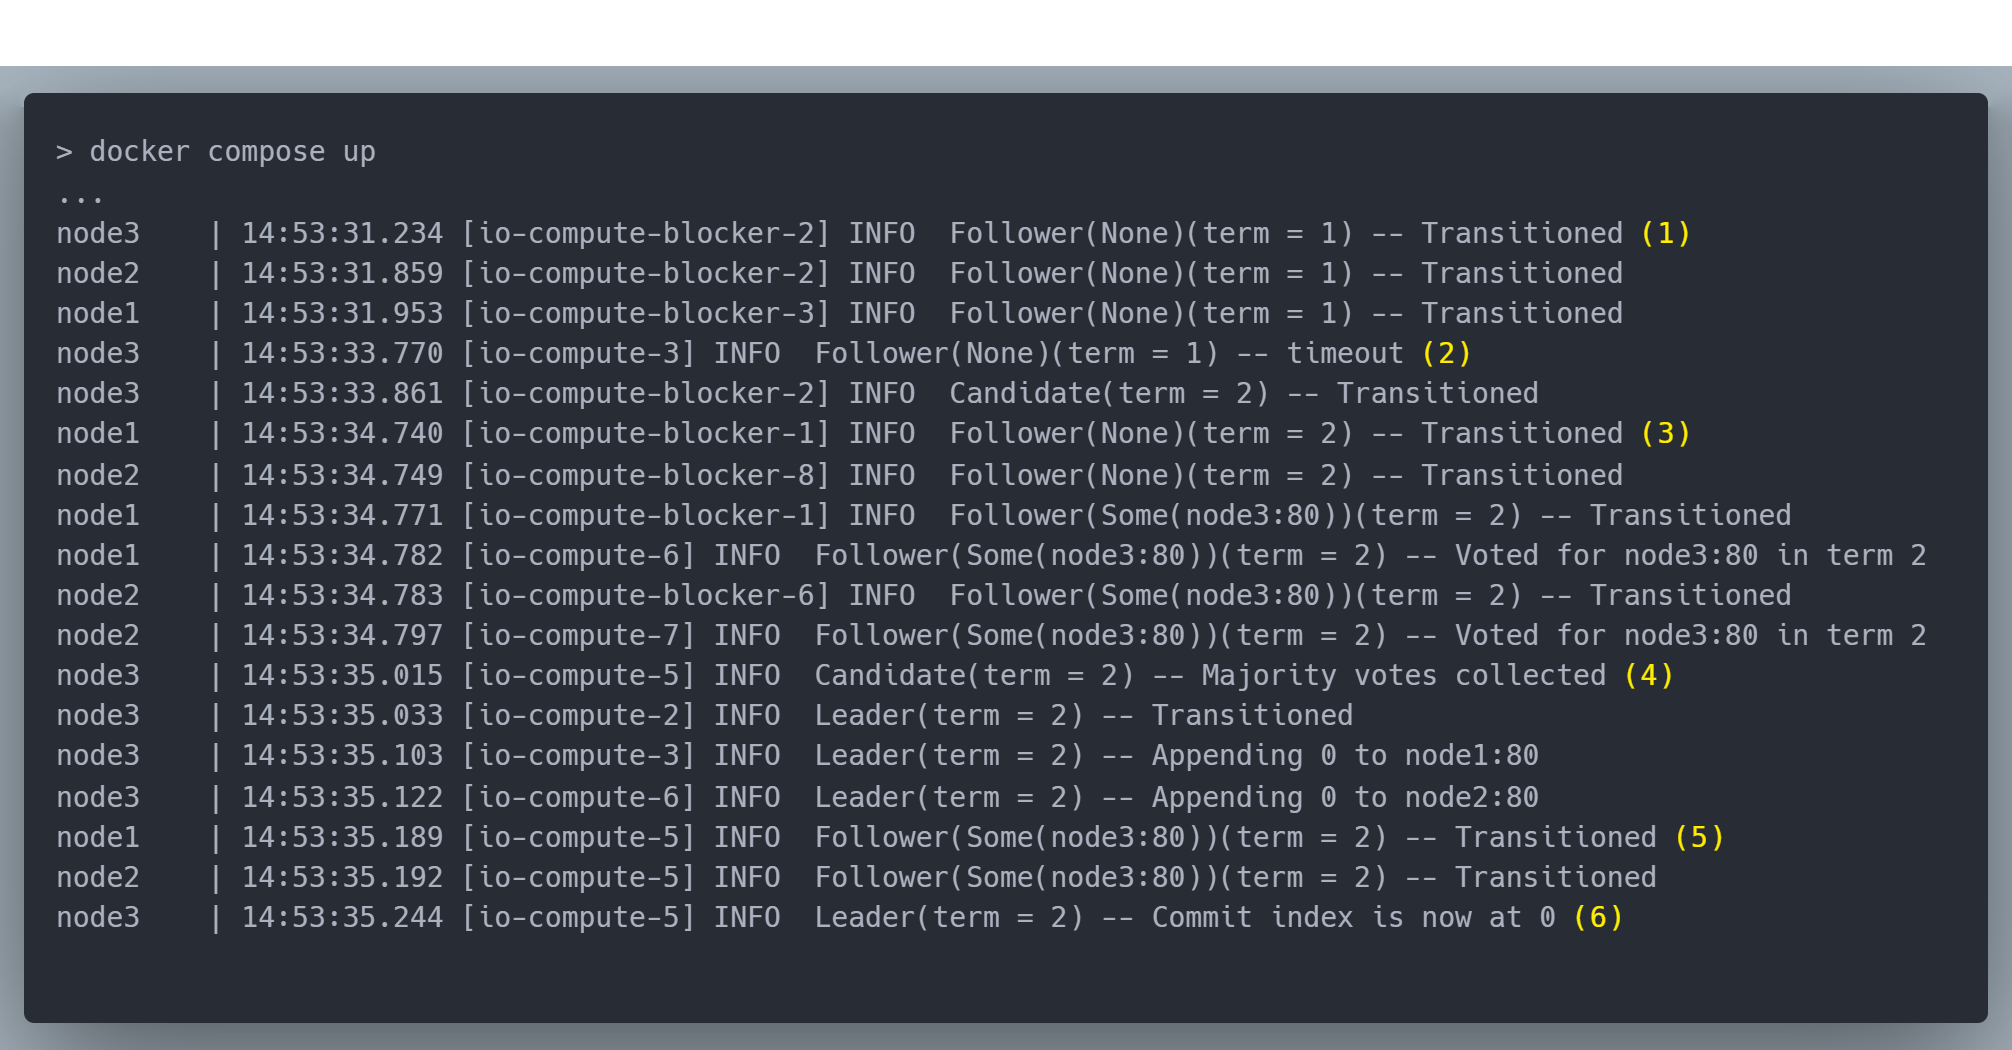
\includegraphics[width=500pt]{images/scenario_1.png}
\caption{Cluster output for the first scenario.}
\label{fig:scenario-1}
\end{figure}

\subsubsection{Result}

In Figure \ref{fig:scenario-1}, the following events are marked:
\begin{enumerate}
    \item After the initial startup, all three servers become followers for the first term.
    \item Since there is no leader in the cluster to send heartbeats, Server 3 becomes a candidate for the second term after an election timeout goes by and starts requesting votes from Server 1 and Server 2.
    \item Server 1 and Server 2 receive the vote requests, transition to followers in the second term, and vote for Server 3.
    \item Having collected votes from the majority, Server 3 transitions to a leader and informs its followers by sending an empty append request, at index 0.
    \item The followers respond to the append requests, recognizing Server 3 as the leader.
    \item Since the leader successfully replicated the entry at index 0, it is marked as committed, and the replicated state machine is ready for further input. The cluster remains stable thereafter, as the leader maintains its authority by sending heartbeat requests in the background.
\end{enumerate}

\subsubsection{Commentary}

Note that the entry at index 0 is virtual; it is not an actual entry in the log. It matches with the position in the follower's log right before the first entry, and the leader replicates it when its own log is empty.

\subsection{Recovery on Single Follower's Crash}

This scenario showcases how a cluster handles a follower's crash and recovery, with no requests being issued in between.

\subsubsection{Initial State}

The replicated log is empty and the cluster is stable with Server 1 as the leader, as shown under Marker 1 in Figure \ref{fig:scenario-2-cluster}.

\subsubsection{Input}

Two commands are executed via the terminal: \lstinline|docker stop node3|, which simulates a crash by stopping the container running Server 3, and \lstinline|docker start node3|, which simulates recovery by starting it up again. These are shown in Figure \ref{fig:scenario-2-commands}. Note that there is a delay of several seconds added between the execution of the two commands.

\begin{figure}[!ht]
\centering
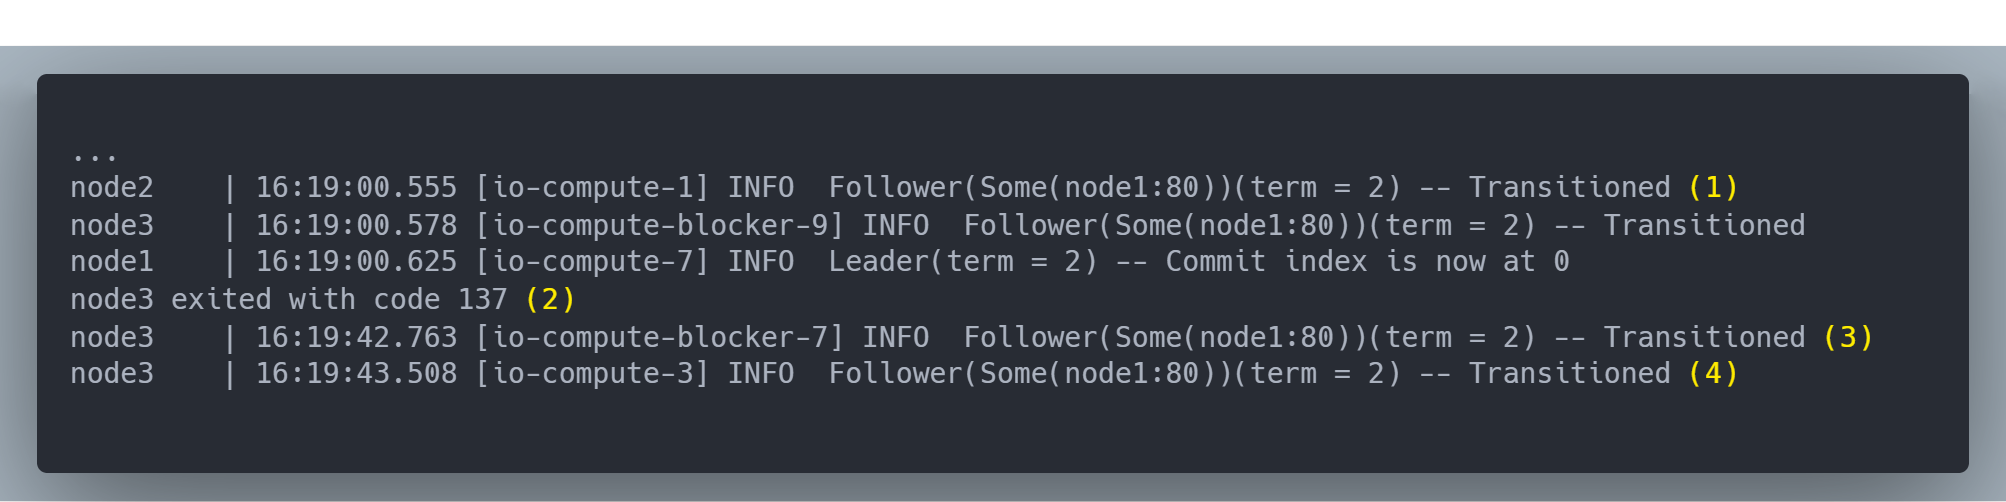
\includegraphics[width=500pt]{images/scenario_2_cluster.png}
\caption{Cluster output for the second scenario.}
\label{fig:scenario-2-cluster}

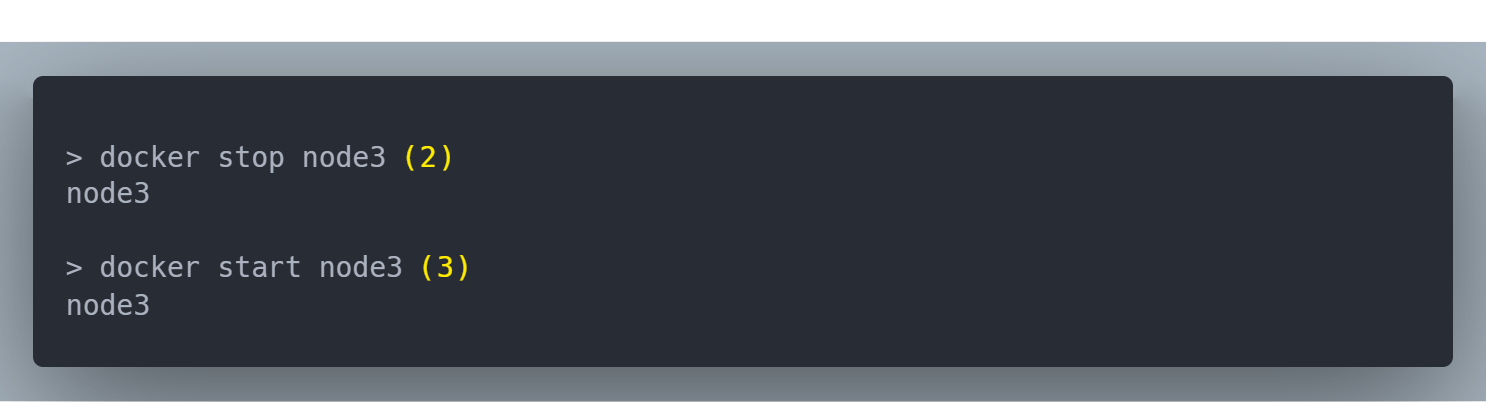
\includegraphics[width=500pt]{images/scenario_2_commands.png}
\caption{Input commands for the second scenario.}
\label{fig:scenario-2-commands}
\end{figure}

\subsubsection{Result}

In Figures \ref{fig:scenario-2-cluster} and \ref{fig:scenario-2-commands}, the following events are marked:
\begin{enumerate}
    \item The cluster is stable before any command is issued, with Server 1 being the leader and Servers 2 and 3 being followers.
    \item Server 3 is stopped via an external command.
    \item After several seconds, Server 3 is started up again.
    \item Server 3 learns again that Server 1 is the leader and remains as a follower. The cluster remains stable thereafter.
\end{enumerate}

\subsubsection{Commentary}

Note that the log message Marked as 4 is produced because the server learns of the leader's location in the cluster. This information is not persisted between server restarts, so it has to be re-learned. This is not clearly shown in the message, but it is proven by the server remaining as a follower and not transitioning to candidate after several election timeouts go by. 

\subsection{Recovery on Multiple Followers' Crash}

This scenario expands on the previous one by showing the cluster's behavior when all followers crash and later recover, with no requests being issued in between.

\subsubsection{Initial State}

The replicated log is empty and the cluster is stable with Server 3 as the leader, as shown under Marker 1 in Figure \ref{fig:scenario-3-cluster}.

\subsubsection{Input}

A crash is simulated in both follower servers by issuing \lstinline|docker stop| commands via the terminal. They are restarted after several seconds, by issuing \lstinline|docker start| commands. These are shown in Figure \ref{fig:scenario-3-commands}.

\begin{figure}[!ht]
\centering
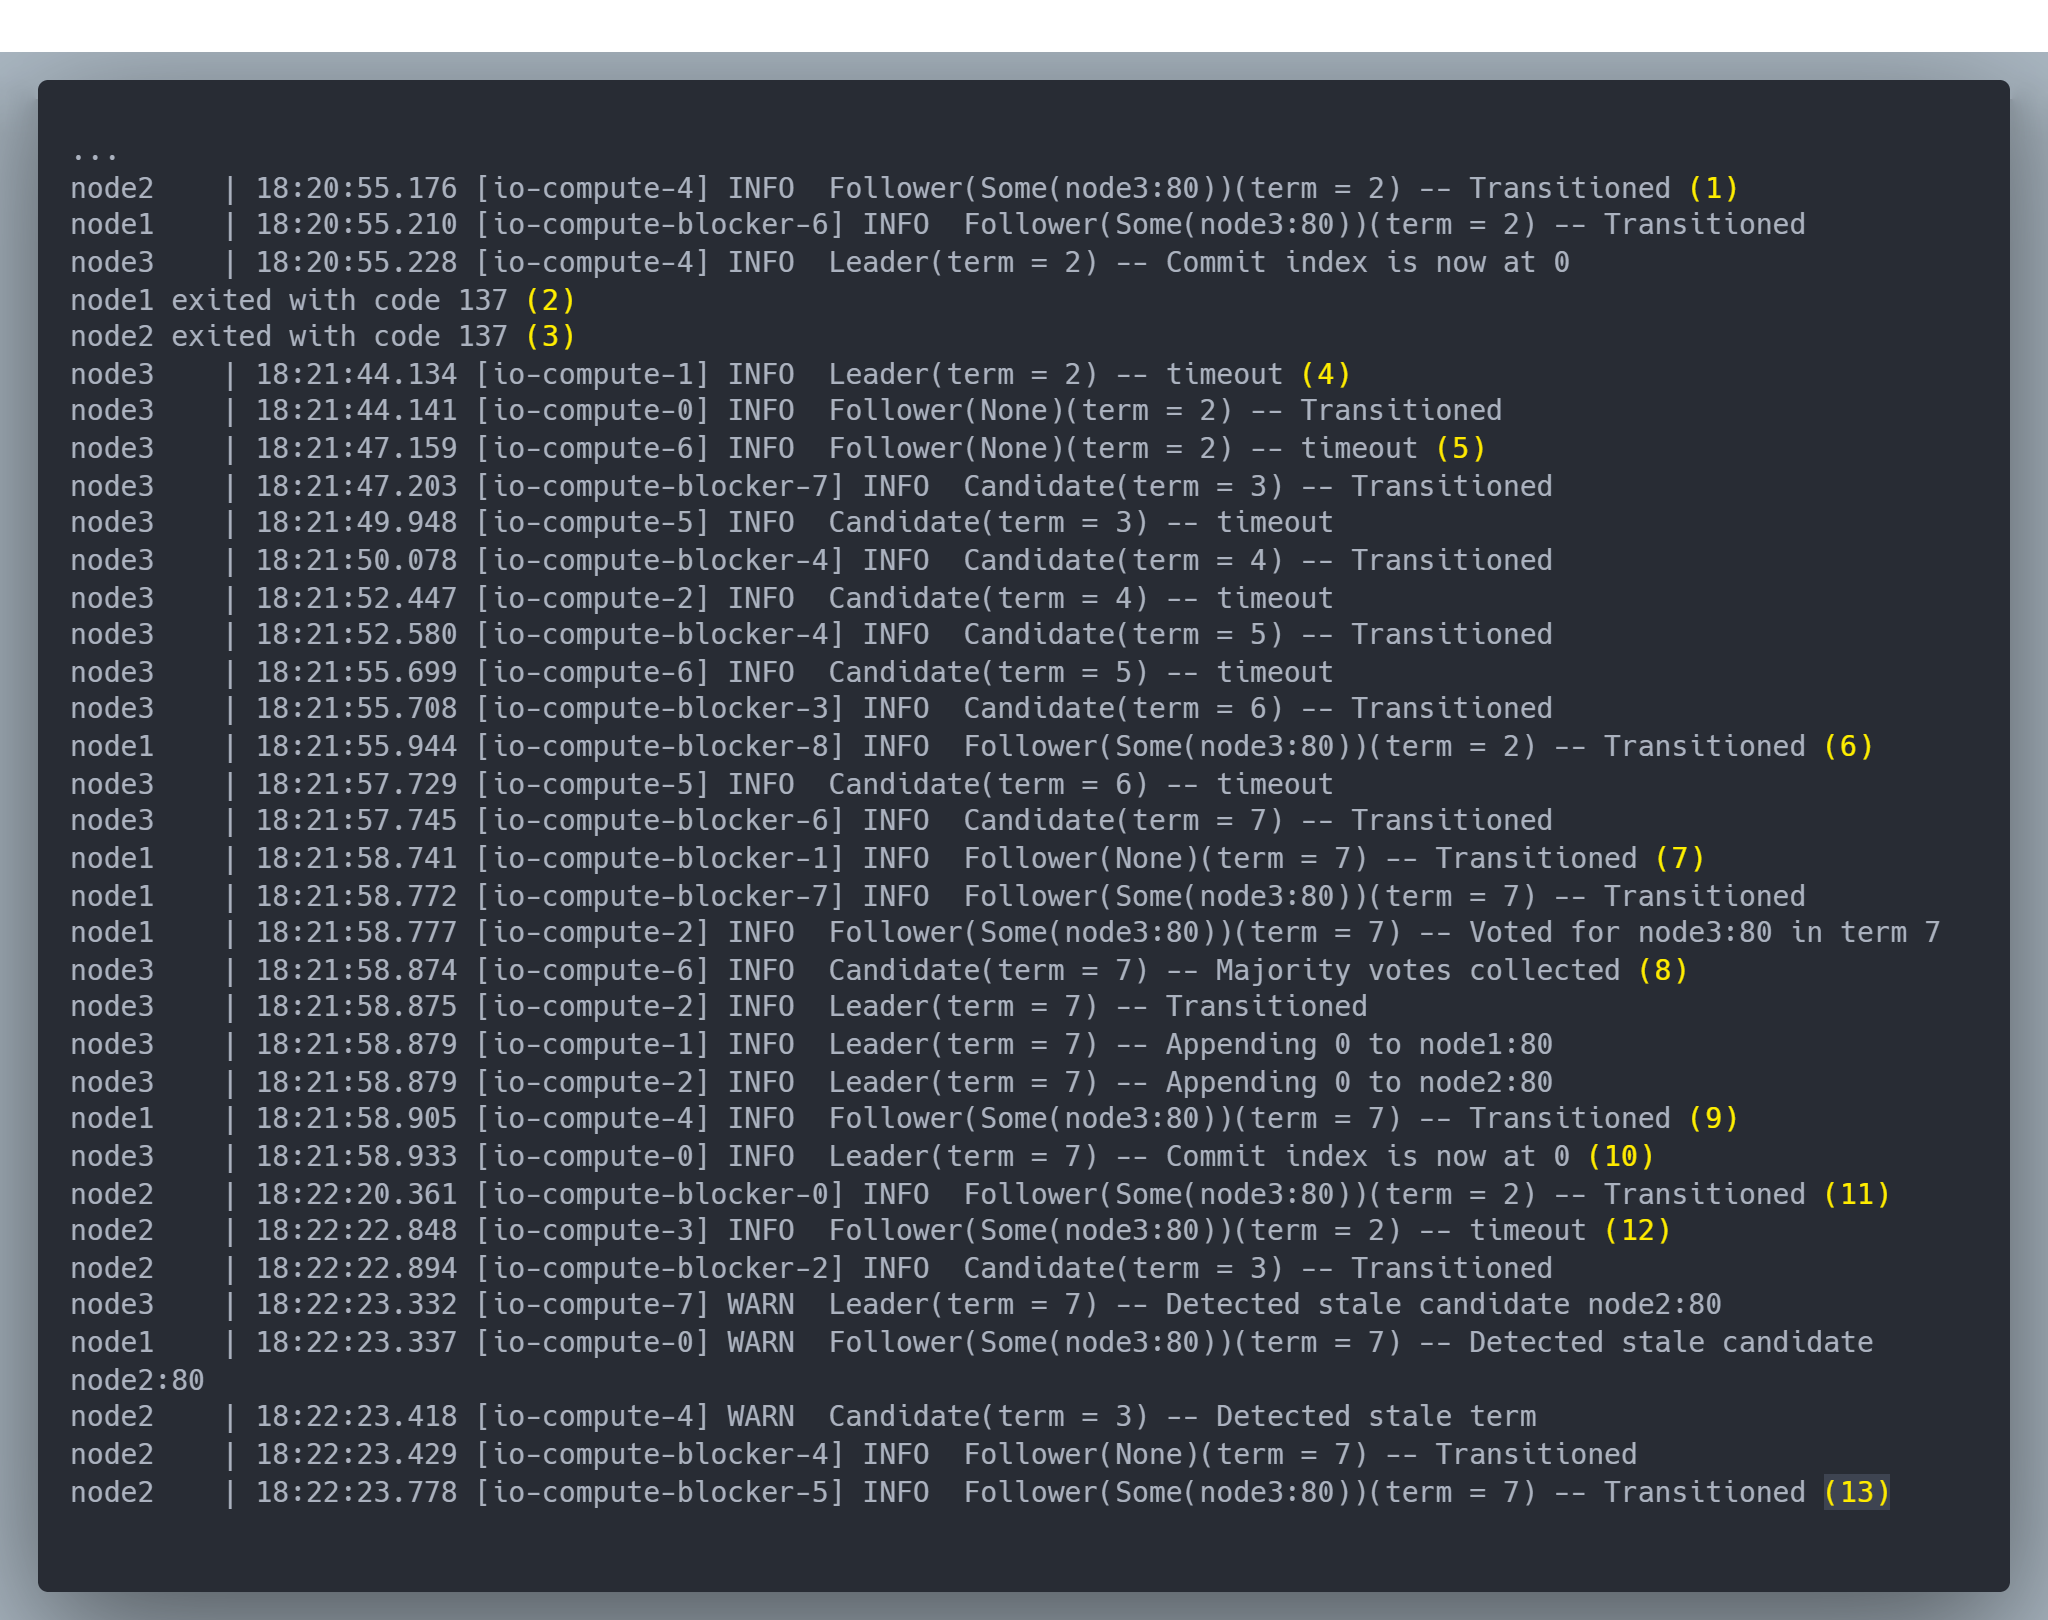
\includegraphics[width=500pt]{images/scenario_3_cluster.png}
\caption{Cluster output for the third scenario.}
\label{fig:scenario-3-cluster}
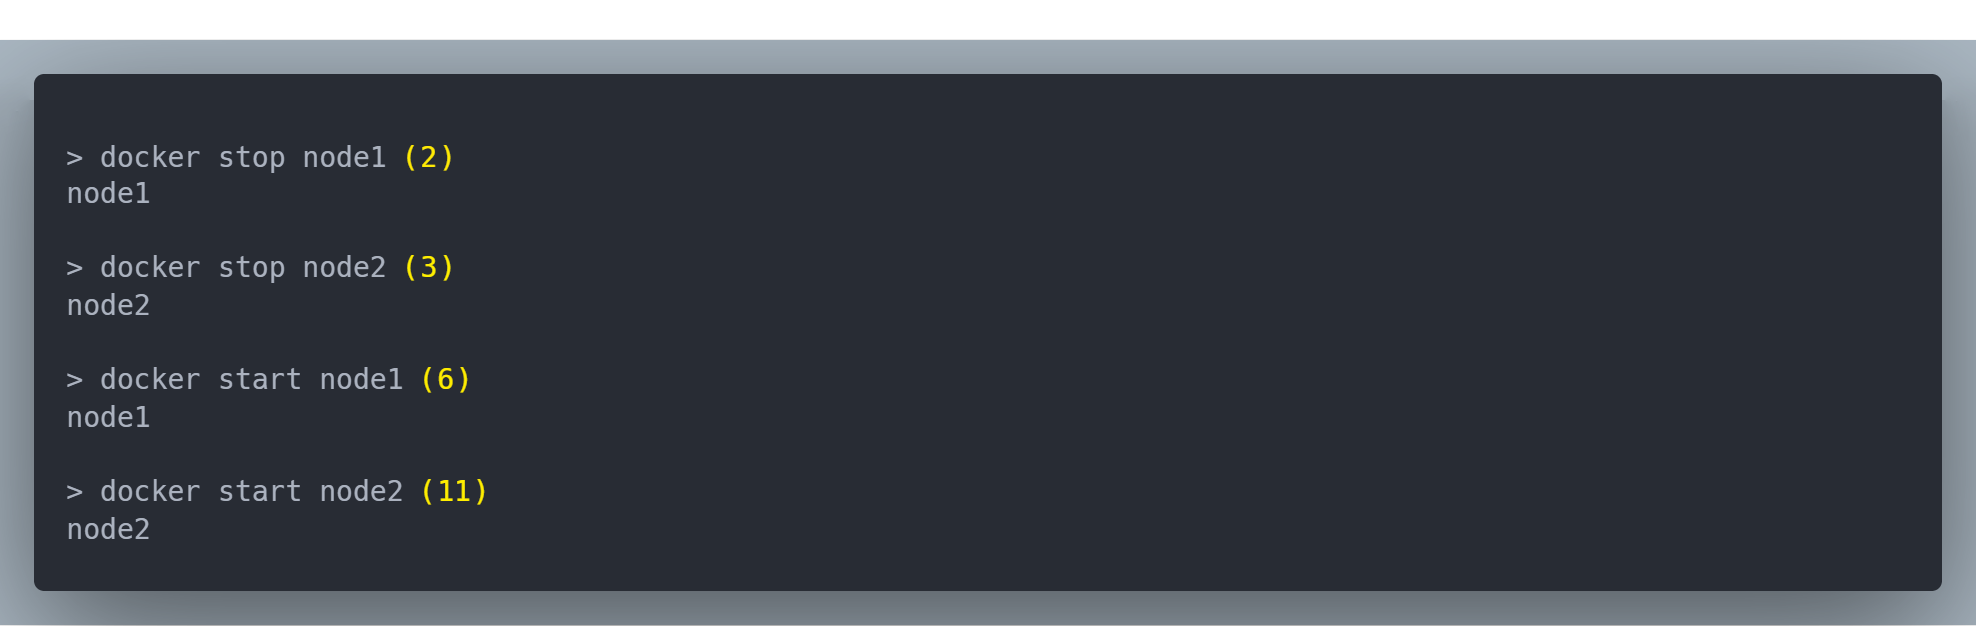
\includegraphics[width=500pt]{images/scenario_3_commands.png}
\caption{Input commands for the third scenario.}
\label{fig:scenario-3-commands}
\end{figure}

\subsubsection{Result}

In Figures \ref{fig:scenario-3-cluster} and \ref{fig:scenario-3-commands}, the following events are marked:
\begin{enumerate}
    \item The cluster is stable before any command is issued, with Server 3 being the leader and Servers 1 and 2 being followers.
    \item Server 1 is stopped via an external command.
    \item Server 2 is stopped via an external command.
    \item Server 3 is unable to reach a majority of the cluster. Since it cannot make progress, it reverts back to a follower for the current term.
    \item Server 3 transitions to a candidate for the next term after an election timeout and tries to gather votes. As no other servers are reachable, Server 3 goes through several election cycles with the term increasing each time, until a majority can be reached again.
    \item Server 1 is started up again. It has a stale term, as it has not observed any of the election cycles.
    \item Server 1 is reached by Server 3, which asks for a vote. Server 1 learns of the current term and votes for Server 3.
    \item Server 3 gathered a vote from Server 1, and since it has also implicitly voted for itself, it has collected a majority of votes and becomes the leader once more. Then, it attempts to replicate the virtual entry to the rest of the cluster, asserting its authority.
    \item Server 1 accepts the virtual entry which informs it that Server 3 is the leader for the current term.
    \item Server 3 has successfully replicated the virtual entry to the majority, so it is marked as committed.
    \item Server 2 is started up again and has a stale term.
    \item Server 2 happened to not observe the leader's heartbeats for an election timeout and transitioned to candidate. However, its vote requests are rejected by all other servers due to its stale term and it reverts to a follower. Additionally, the other servers inform Server 2 of the current term, so Server 2 adopts it.
    \item Server 2 finally receives heartbeats from the leader and recognizes it, remaining as a follower. The cluster then remains stable indefinitely.
\end{enumerate}

\subsubsection{Commentary}

These results show that in Raft clusters, and in distributed systems more broadly, there are hiccups during the consensus process that may cause a temporary divergence. However, Raft, and all successful consensus systems, guarantee that the servers will eventually reach a correct state.\\

In particular, events 11 and 12 show that Server 2 mistakenly became a candidate, which could be catastrophic in a naively implemented system. The candidate could gather votes and erroneously modify the replicated state machine, beginning at a stale view of the log. Raft guards against this type of error through its use of terms and its restrictions in the leader election and log replication processes, described in Chapter 2. As a result, stale servers cannot modify the replicated state machine, and the cluster will eventually be made consistent.

\subsection{Recovery on Leader's Crash}

This scenario showcases the cluster's recovery after the leader crashes. Additionally, it shows how a server that crashed while being the leader can later rejoin the cluster.

\subsubsection{Initial State}

The replicated log is empty and the cluster is stable with Server 1 as the leader, as shown under Marker
1 in Figure \ref{fig:scenario-4-cluster}.

\subsubsection{Input}

The leader is stopped via the terminal by issuing a \lstinline|docker stop| command. It is restarted after several seconds by issuing a \lstinline|docker start| command. These are shown in Figure \ref{fig:scenario-4-commands}.

\begin{figure}[!ht]
\centering
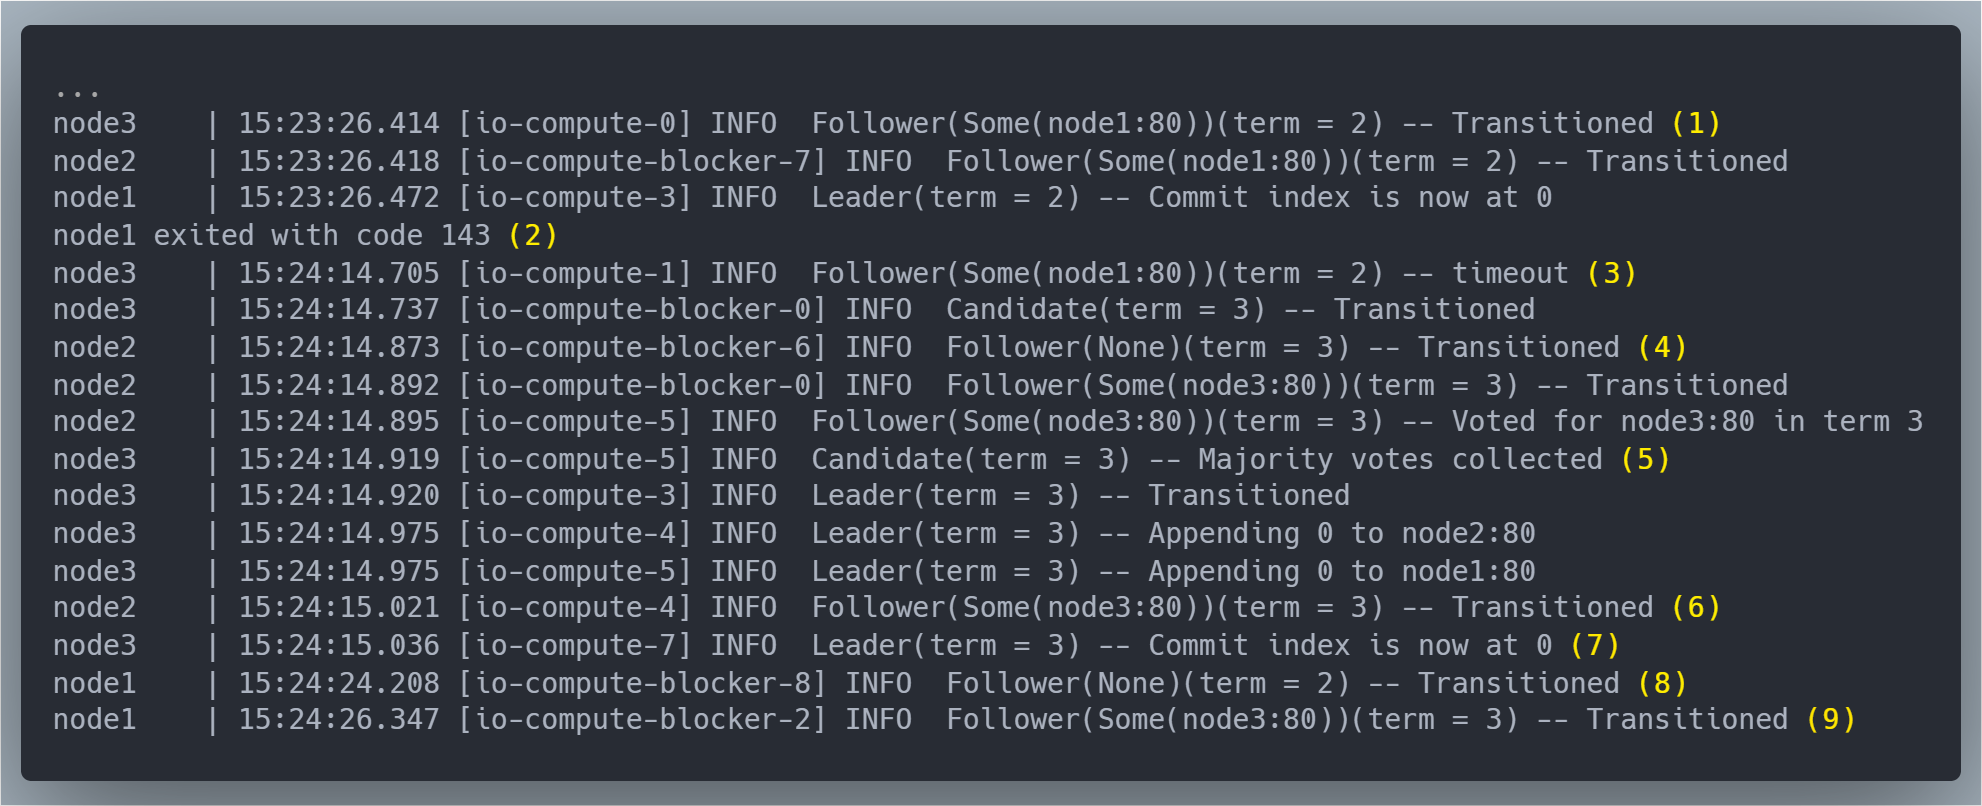
\includegraphics[width=500pt]{images/scenario_4_cluster.png}
\caption{Cluster output for the fourth scenario.}
\label{fig:scenario-4-cluster}
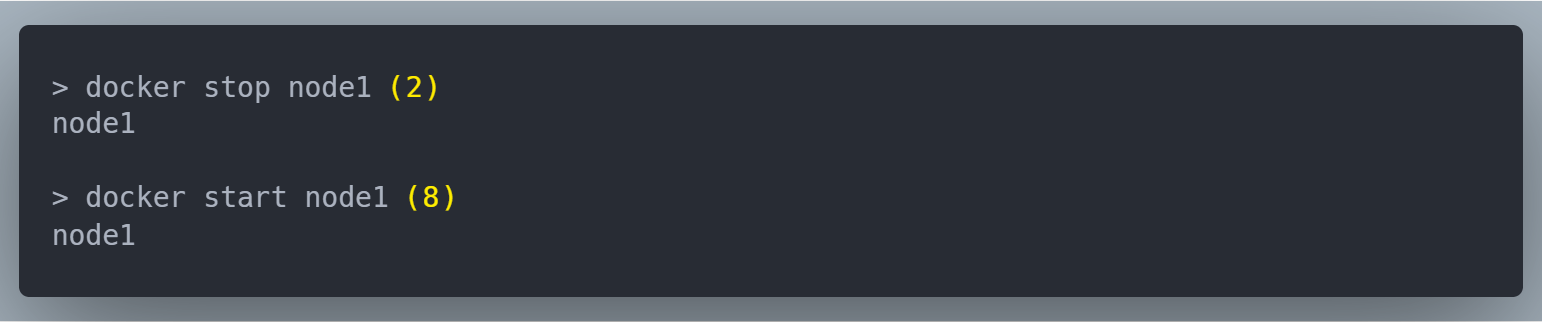
\includegraphics[width=500pt]{images/scenario_4_commands.png}
\caption{Input commands for the fourth scenario.}
\label{fig:scenario-4-commands}
\end{figure}

\subsubsection{Result}

In Figures \ref{fig:scenario-4-cluster} and \ref{fig:scenario-4-commands}, the following events are marked:
\begin{enumerate}
    \item The cluster is stable before any command is issued, with Server 1 being the leader and Servers 2 and 3 being followers.
    \item Server 1 is stopped via an external command.
    \item Server 3 detects that there is no viable leader, as it did not receive heartbeats for an election timeout. It then transitions to a candidate for the next term and requests that the rest of the cluster votes for it.
    \item Server 2 receives the vote request, learns the new term, and votes for Server 3.
    \item Server 3 has gathered votes from the majority of the cluster, as it has also implicitly voted for itself. It then transitions to a leader for the term, and it appends the virtual entry to the rest of the cluster, as its log is still empty.
    \item Server 2 accepts the append from Server 3, recognizing it as the leader.
    \item Server 3 successfully committed the virtual entry, as it is replicated to the majority of the cluster, including itself.
    \item Server 1 is started up again via an external command and joins the cluster as a follower. Its term is stale, since it did not observe any of the previous transitions.
    \item Server 1 receives a heartbeat from Server 3 and recognizes it as the leader. The cluster remains stable thereafter.
\end{enumerate}

\subsubsection{Commentary}

This scenario shows one of the fundamental requirements for a successful leader-based consensus system; progress continues even when the current leader fails by quickly and safely electing a new one.

\subsection{Recovery after Complete Cluster Termination}

This scenario showcases the cluster's ability to progress after completely failing and becoming operational again.

\subsubsection{Initial State}

The replicated log is empty and the cluster is stable with Server 2 as the leader, as shown under Marker 1 in Figure \ref{fig:scenario-5-cluster}.

\subsubsection{Input}

The entire cluster is completely shut down by issuing the \lstinline|docker compose down| command. After several seconds, the cluster is restarted by issuing the \lstinline|docker compose up -d| command. These are shown in Figure \ref{fig:scenario-5-commands}.

\begin{figure}[!ht]
\centering
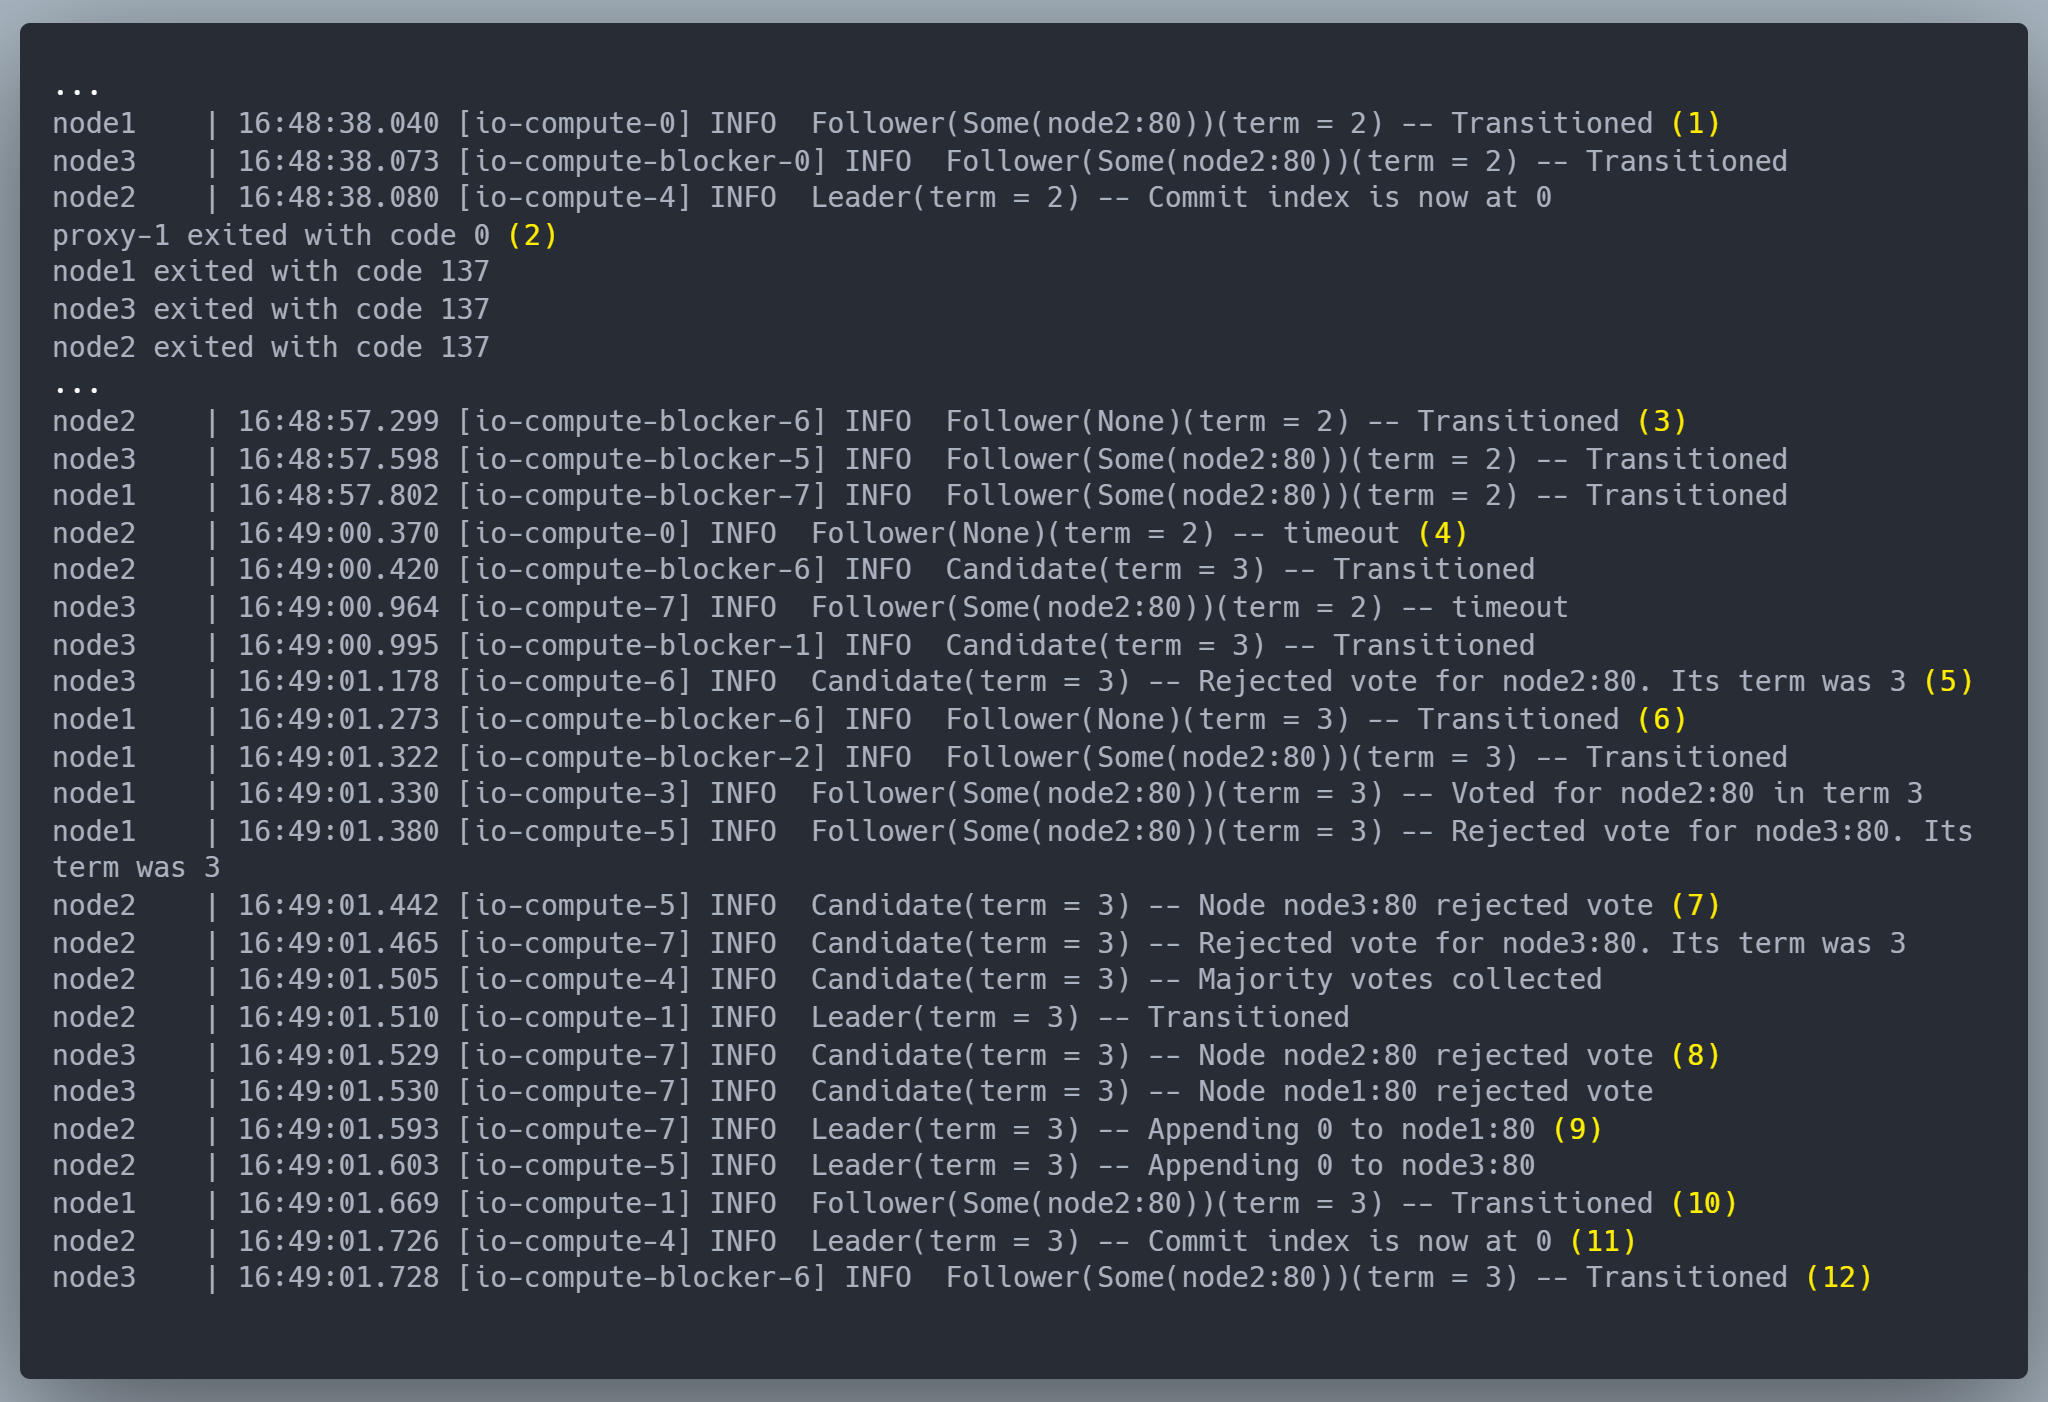
\includegraphics[width=500pt]{images/scenario_5_cluster.png}
\caption{Cluster output for the fifth scenario.}
\label{fig:scenario-5-cluster}
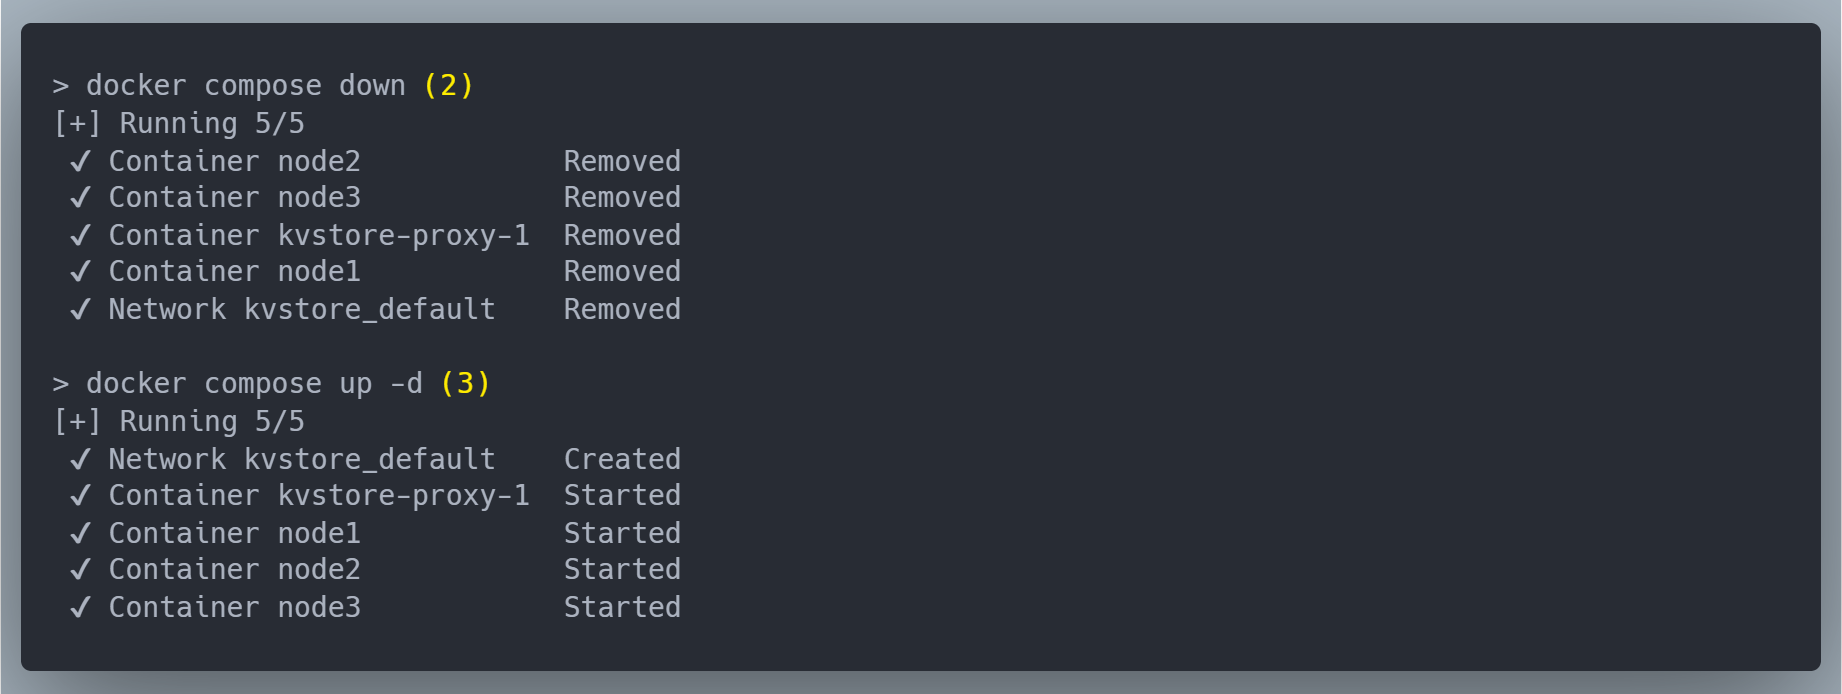
\includegraphics[width=500pt]{images/scenario_5_commands.png}
\caption{Input commands for the fifth scenario.}
\label{fig:scenario-5-commands}
\end{figure}

\subsubsection{Result}

In Figures \ref{fig:scenario-5-cluster} and \ref{fig:scenario-5-commands}, the following events are marked:
\begin{enumerate}
    \item The cluster is stable before any command is issued, with Server 2 being the leader and Servers 1 and 3 being followers. The Servers have reached the second term, since an election cycle happened during startup.
    \item The cluster is shut down via an external command.
    \item After several seconds, the cluster is restarted via an external command. All servers join as followers with the term they knew of before they were shut down.
    \item Both Server 2 and Server 3 experience election timeouts in quick succession. They transition to candidates for the next term and attempt to gather votes.
    \item Server 3 rejects to vote for Server 2, as it has already implicitly voted for itself.
    \item Server 1 receives the vote request from Server 2 before the request from Server 3. It then grants the vote to Server 2 and rejects Server 3.
    \item Server 2 learns that Server 3 rejected its vote request, but Server 1 granted it. Since Server 2 has also implicitly voted for itself, it has received votes by the majority, and it transitions to a leader for the term. Server 2 also rejects the vote request it received from Server 3.
    \item Server 3 learns of the other servers' rejections. Since it has not received a majority of votes, it remains as a candidate.
    \item Server 2, acting as a leader, starts appending the virtual entry to other servers, informing them of its victory.
    \item Server 1 responds to the append from Server 2, recognizing it as the leader.
    \item After Server 1 responds, the leader has successfully committed the virtual entry.
    \item Server 3 also responds to the append from Server 2, recognizing it as the leader and transitioning to a follower.
\end{enumerate}

\subsubsection{Commentary}

These results show how the persistence layer is used to preserve any required information through complete system crashes or restarts. It also showcases how the leader election process, as defined by Raft, succeeds, even when an unfortunate timing of the election timeouts leads to multiple candidates for a term.

\subsection{Simple Get and Put Commands} \label{simple-get-put-scenario} \label{L-flag}

This scenario showcases the key-value store in action by issuing simple read and write requests.

\subsubsection{Initial State}

The replicated log is empty and the cluster is stable with Server 1 as the leader, as shown under Marker 1 in Figure \ref{fig:scenario-6-cluster}.

\subsubsection{Input}

As shown in Figure \ref{fig:scenario-6-commands}, the \lstinline|curl| command is used to send HTTP requests to the store. Additionally, the \lstinline|uuidgen| command is used to generate unique command identifiers, which are required for enforcing linearizable semantics, as detailed in Section \ref{linearizable-semantics}.\\

All commands are issued with the \lstinline|-L| flag, instructing \lstinline|curl| to follow redirects. This is necessary as requests are issued against the proxy without specifying the target server. If the server to which the proxy initially routes the request is not the leader, it returns a redirection response. Curl then follows this redirection response and addresses the leader directly.\\

Note that it is possible to find out the location of the current leader once and then address it directly without further redirections. However, this was avoided to keep the demonstration simple.

\begin{figure}[!ht]
\centering
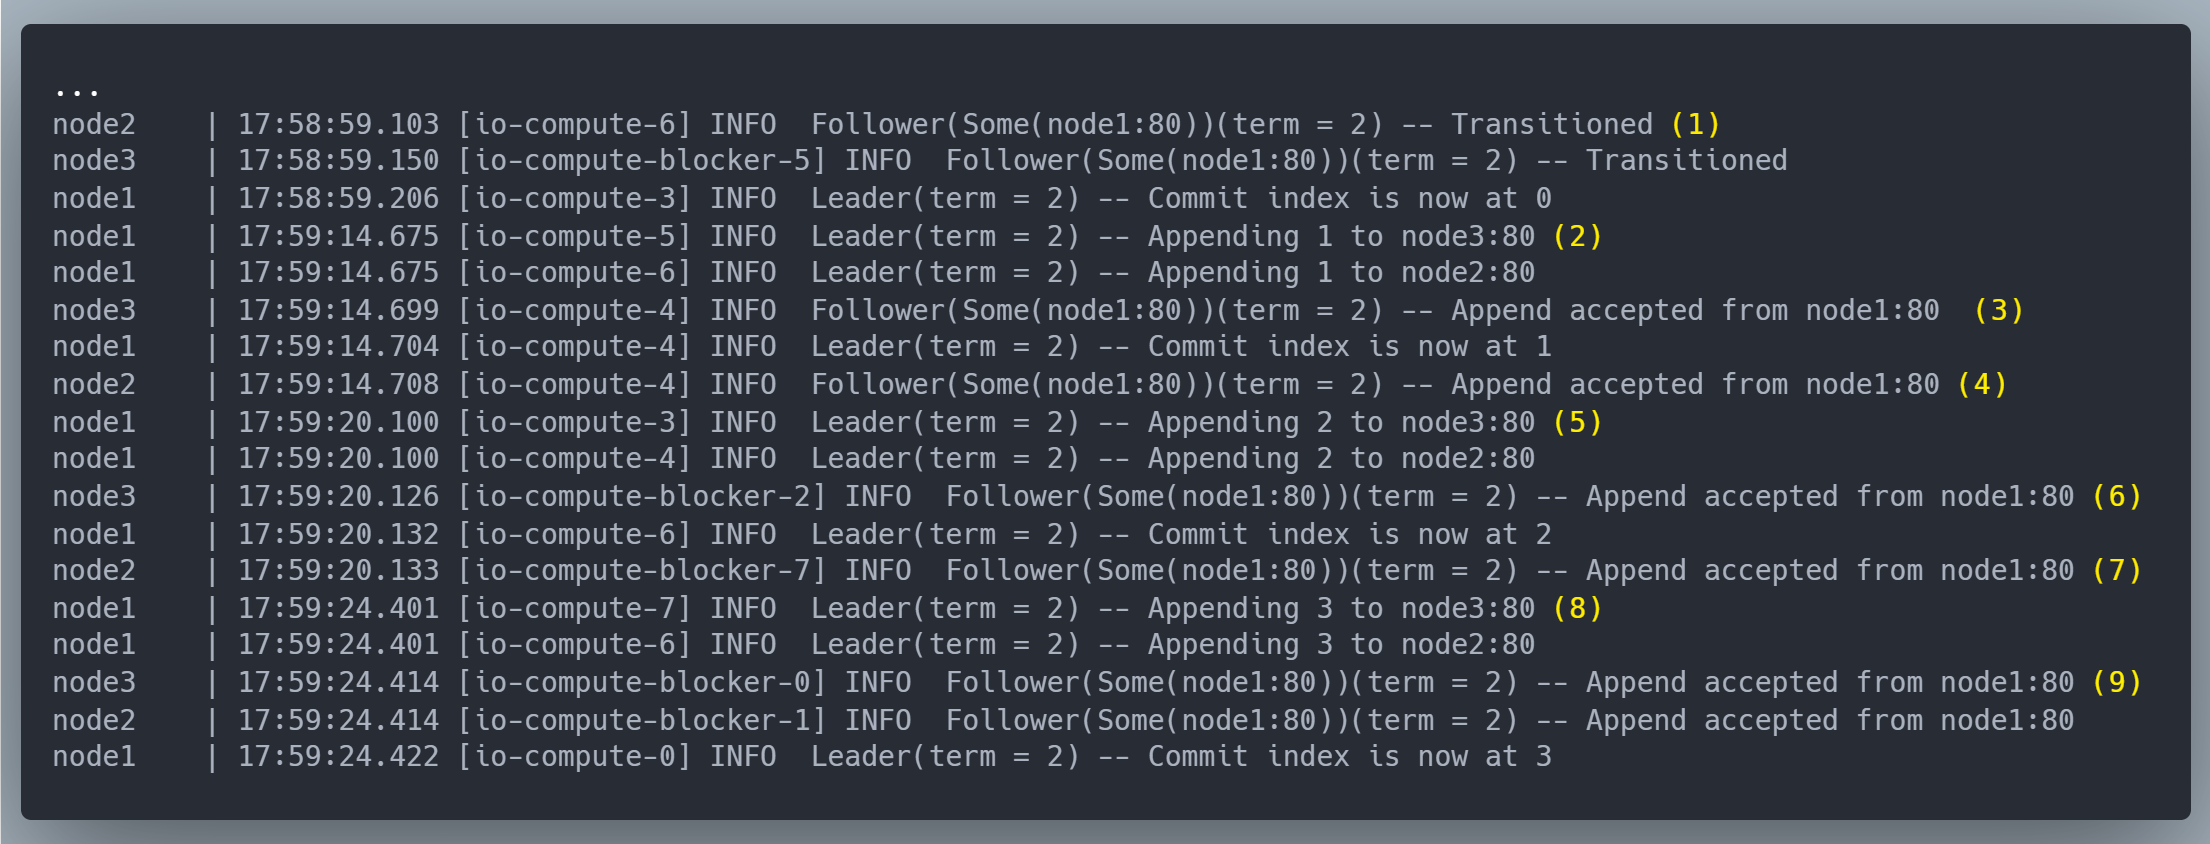
\includegraphics[width=500pt]{images/scenario_6_cluster.png}
\caption{Cluster output for the sixth scenario.}
\label{fig:scenario-6-cluster}
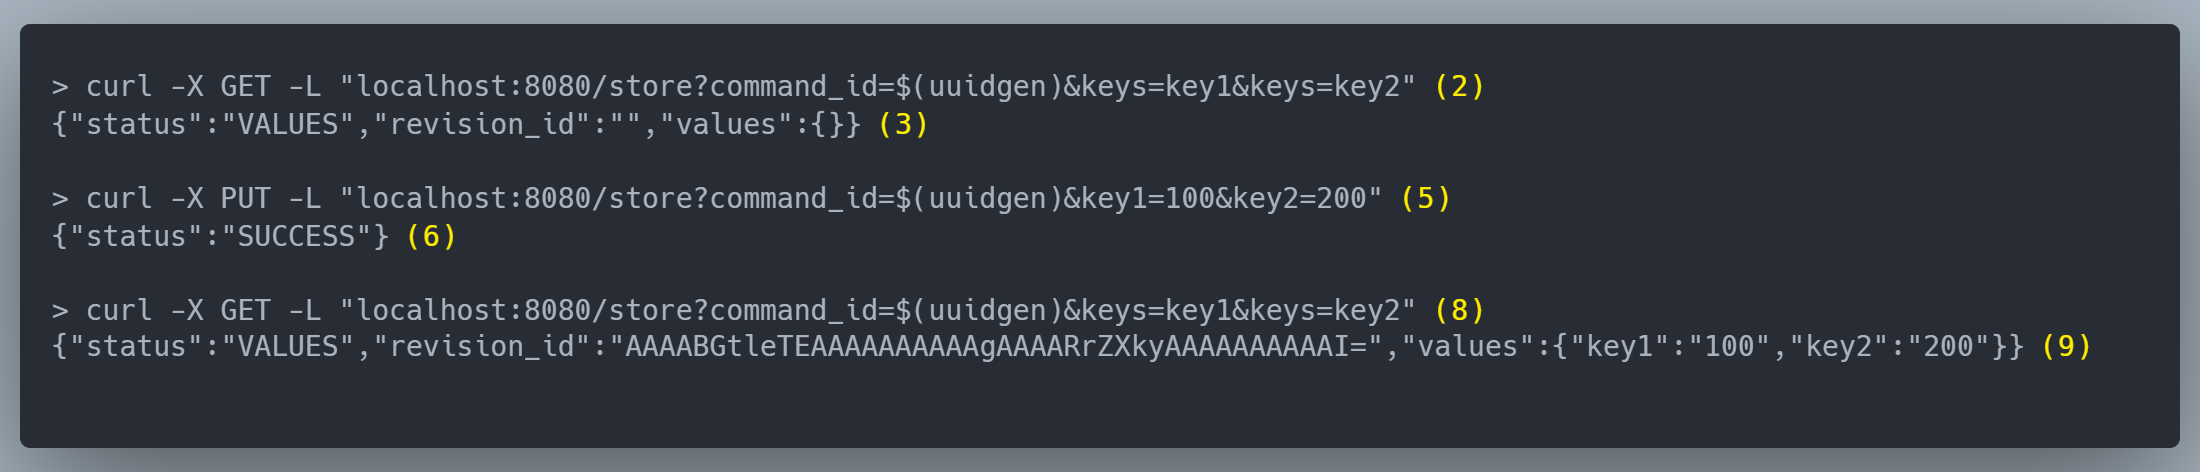
\includegraphics[width=500pt]{images/scenario_6_commands.png}
\caption{Input commands for the sixth scenario.}
\label{fig:scenario-6-commands}
\end{figure}

\subsubsection{Result}
In Figures \ref{fig:scenario-6-cluster} and \ref{fig:scenario-6-commands}, the following events are marked:
\begin{enumerate}
    \item The cluster is stable before any command is issued, with Server 1 being the leader and Servers 2 and 3 being followers.
    \item A client requests to view the values for keys \lstinline|key1| and \lstinline|key2|. As detailed in Section \ref{linearizable-semantics}, read requests are committed to the replicated log like any other command, so the replication process begins; Server 1, acting as the leader, sends append requests to its followers.
    \item Server 3 accepts the append first, inserting the command to its internal log, and responding to the leader. After this follower's response, the leader has successfully replicated the command to the majority of the cluster, including itself, and it increments the commit index. At that point, the client receives a response to its request, which contains no key-value pairs, since the store is empty.
    \item Server 2 also accepts the leader's append request.
    \item A client requests to insert the key-value pairs \lstinline|(key1,100)| and \lstinline|(key2,200)|. The replication process for the command begins with the leader sending append requests to its followers.
    \item Server 3 accepts the append first, inserting the command to its internal log, and responding to the leader. After this follower's response, the command is deemed committed, and the commit index is incremented. At that point, the client receives a response to its request, which shows that the insertion was successful.
    \item Server 2 also accepts the leader's append request.
    \item A client requests to view the values for keys \lstinline|key1| and \lstinline|key2|. The replication process for the command begins with the leader sending append requests to its followers.
    \item Both followers accept the append in quick succession, inserting the command to their internal logs, and responding to the leader. After the followers' responses, the leader has successfully replicated the command to the cluster and it increments the commit index. At that point, the client receives a response to its request, showing the requested key-value pairs. Along with the pairs, a revision id is returned, which marks the returned keys' current state.
\end{enumerate}

\subsection{Concurrent Get and Put Commands}

This scenario shows the store's behavior when multiple clients attempt to modify it concurrently, without using the provided transaction mechanism. It should show that the store reaches consensus properly about the replicated log, but the resulting state of the store is not the expected one, clearly showing the need for transactions.

\subsubsection{Initial State}

The replicated log is empty and the cluster is stable with Server 3 as the leader, as shown under Marker 1 in Figure \ref{fig:scenario-7-cluster}.

\subsubsection{Input}

The script \lstinline{concurrent_read_writes} is used for performing reads and writes concurrently. It interacts with the key-value store via HTTP requests, similarly to the previous scenario. Its source code can be found in the GitHub repository \cite{stoufexis-raft}.\\

The script takes three positional parameters: a string instructing to use or not use transactions, the number of keys to modify, and the number of processes concurrently modifying each key. The script figures out exactly which keys it will read and write to by starting at \lstinline|key1| and incrementing it until it has reached the number in the second parameter.\\

In the command shown in Figure \ref{fig:scenario-7-commands}, transactions are turned off, the set of keys from \lstinline|key1| to \lstinline|key10| is picked, and 10 concurrent processes are assigned to each key. In total, 100 processes will be running concurrently, which the script calls "workers".\\

As soon as the command is issued, the script initializes all keys to a value of 1 via a \lstinline|PUT| request. Then, it starts all concurrent processes, with each one reading the key's current value using a \lstinline|GET| request, incrementing it by 1, and inserting the result using a \lstinline|PUT| request. In the end, it reads all keys again, returning their final values. The goal is for each key to reach a value of 11, since they are all incremented 10 times, once by each worker.

\begin{figure}[!ht]
\centering
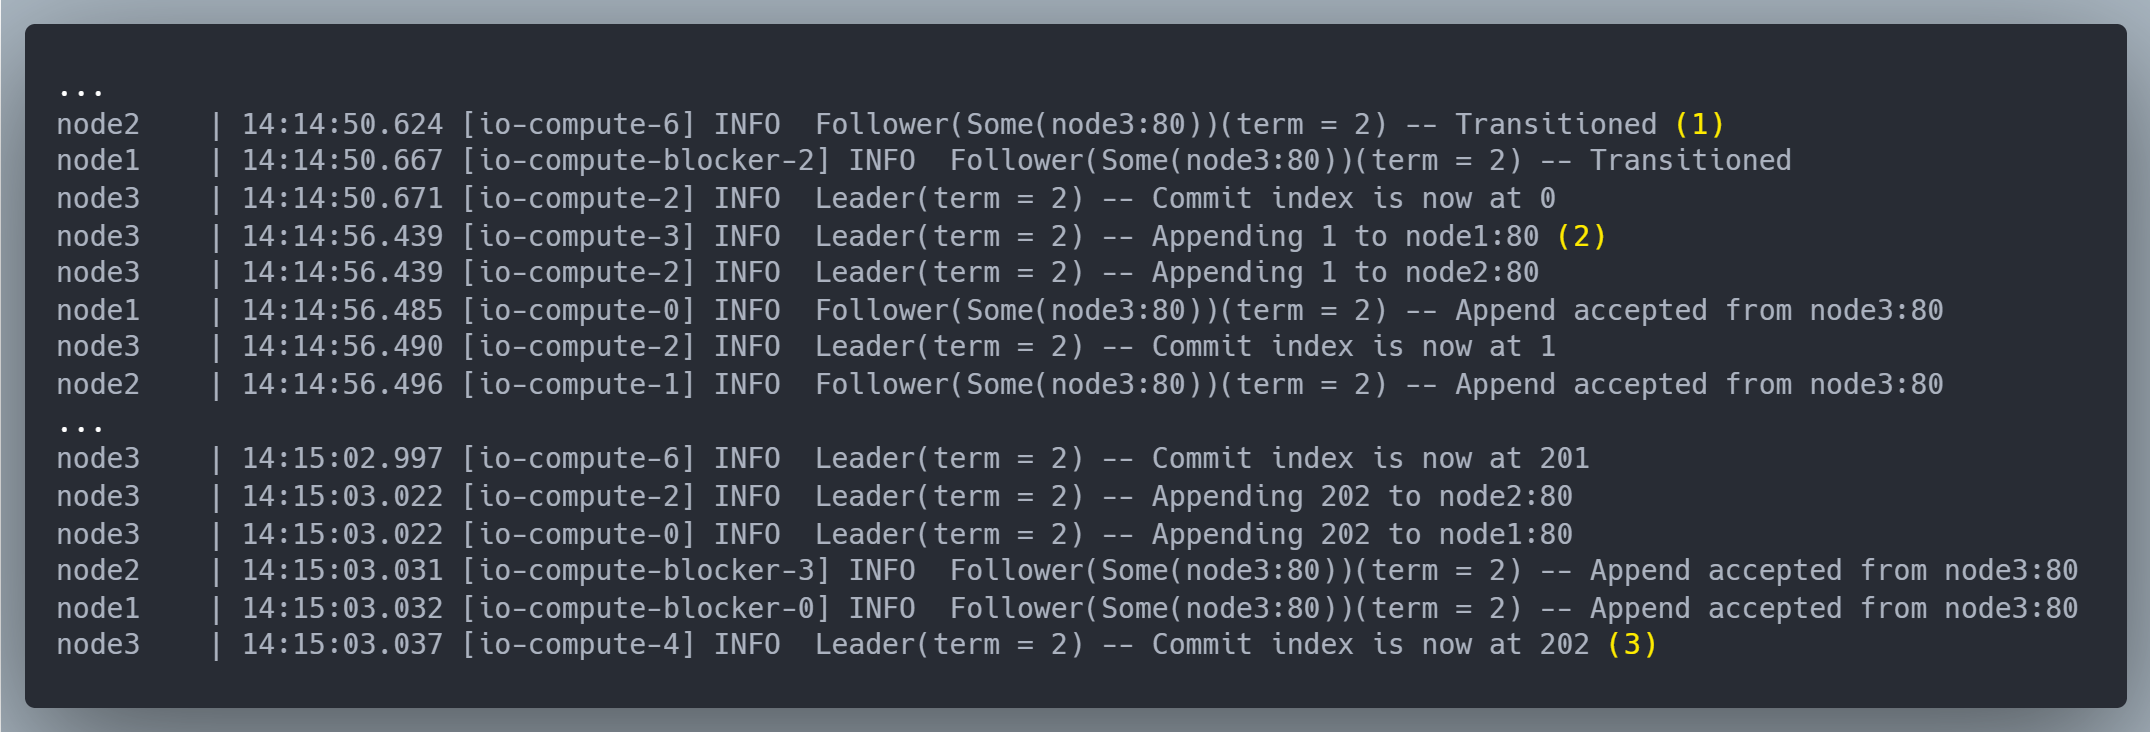
\includegraphics[width=500pt]{images/scenario_7_cluster.png}
\caption{Cluster output for the seventh scenario.}
\label{fig:scenario-7-cluster}
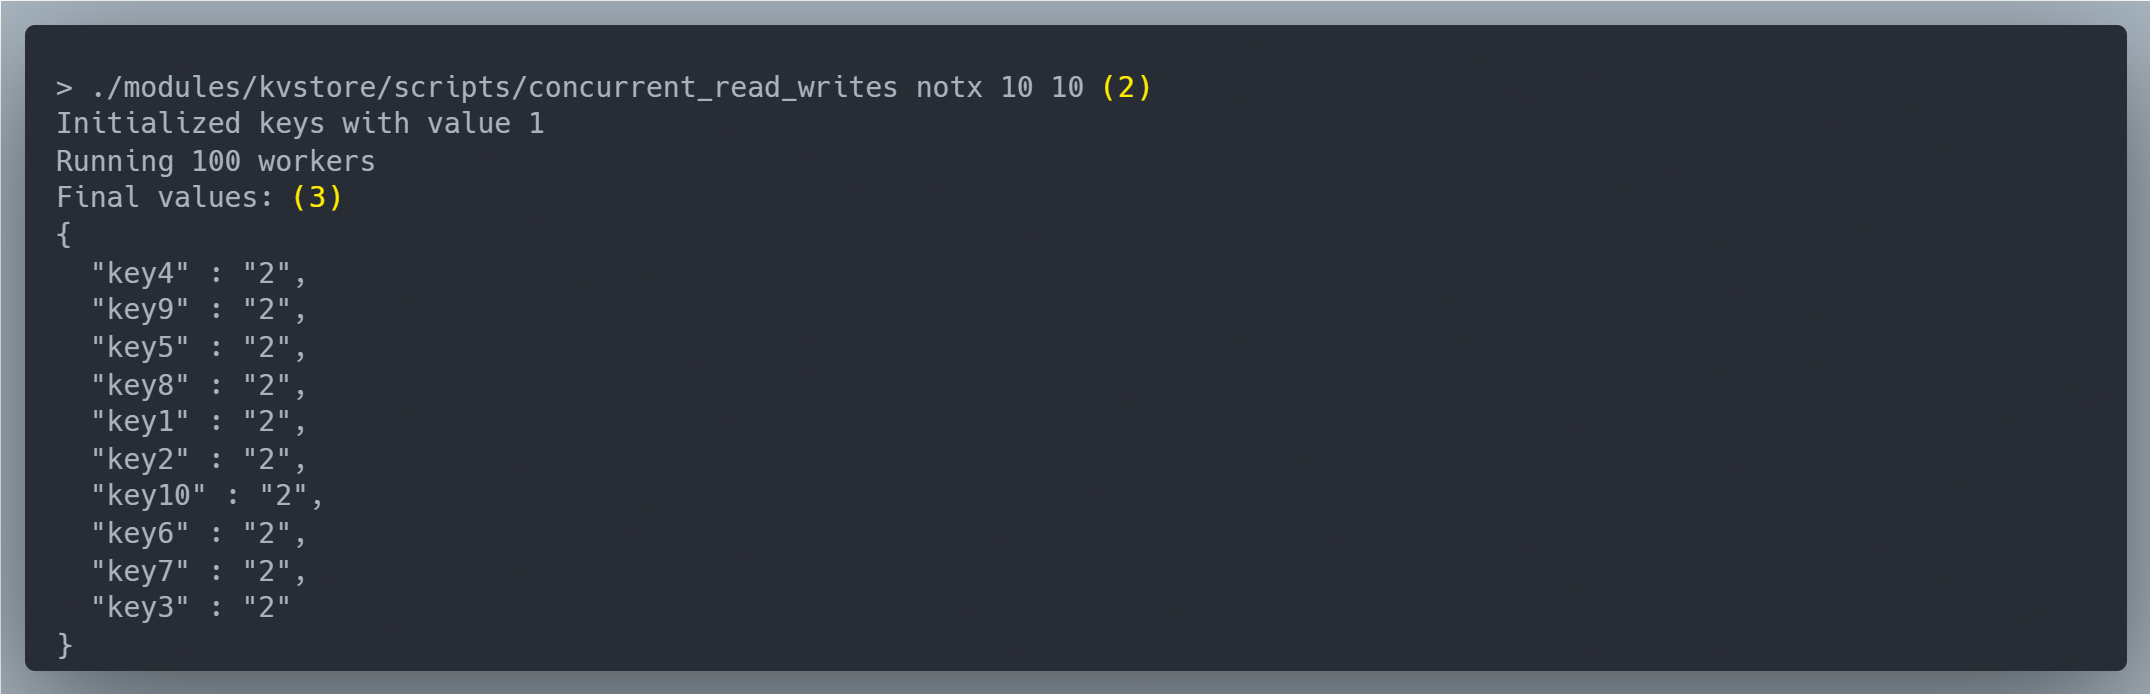
\includegraphics[width=500pt]{images/scenario_7_commands.png}
\caption{Input commands for the seventh scenario.}
\label{fig:scenario-7-commands}
\end{figure}

\subsubsection{Result}
In Figures \ref{fig:scenario-7-cluster} and \ref{fig:scenario-7-commands}, the following events are marked:
\begin{enumerate}
    \item The cluster is stable before any command is issued, with Server 3 being the leader and Servers 1 and 2 being followers.
    \item The script is run externally, which initializes the key-set and then starts up the concurrent workers.
    \item When all 202 commands have been processed, the script reads the keys' final values and returns them.
\end{enumerate}

\subsubsection{Commentary}
Several things are noteworthy in these results. First, in Figure \ref{fig:scenario-7-cluster}, it's shown that the commit index ends up at 202. This is correct, as there was one command issued for the initialization of the keys, 200 commands issued by the 10 concurrent processes, and one command issued for reading the final values. The concurrent processes issued 10 pairs of reads and writes for each key.\\

These results also prove that the Raft implementation is capable of handling concurrent requests from clients, since it reached consensus on the replicated log. However, in this case, the final values are not the desired ones. As transactions were turned off, each read and write pair did not get executed atomically, meaning that each worker ignored the other workers' modifications. In detail, this is what took place:
\begin{enumerate}
    \item All workers read the initial value of 1, before it is incremented.
    \item All workers calculate the incremented value as 2.
    \item Each worker updates the key's value to 2, not knowing that other modifications happened after the initial value was read.
\end{enumerate}

This should clearly demonstrate that a transaction mechanism is necessary to simultaneously support both concurrency and atomicity.

\subsection{Concurrent, Transactional Get and Put Commands} \label{transactions-scenario}
This scenario expands on the previous one by repeating the same actions, but this time using transactions. It should show that each read and write pair is retried until it is made atomically, leading to the expected final value.

\subsubsection{Initial State}

The replicated log is empty and the cluster is stable with Server 1 as the leader, as shown under Marker 1 in Figure \ref{fig:scenario-8-cluster}.

\subsubsection{Input}

As in the previous scenario, the script \lstinline{concurrent_read_writes} is used. However, as shown in Figure \ref{fig:scenario-8-commands}, this time it is instructed to use transactions. Transactions, as described in Section \ref{implementing-transactions}, ensure that each update is executed only if it is made atomically with the preceding read.\\

\begin{figure}[!ht]
\centering
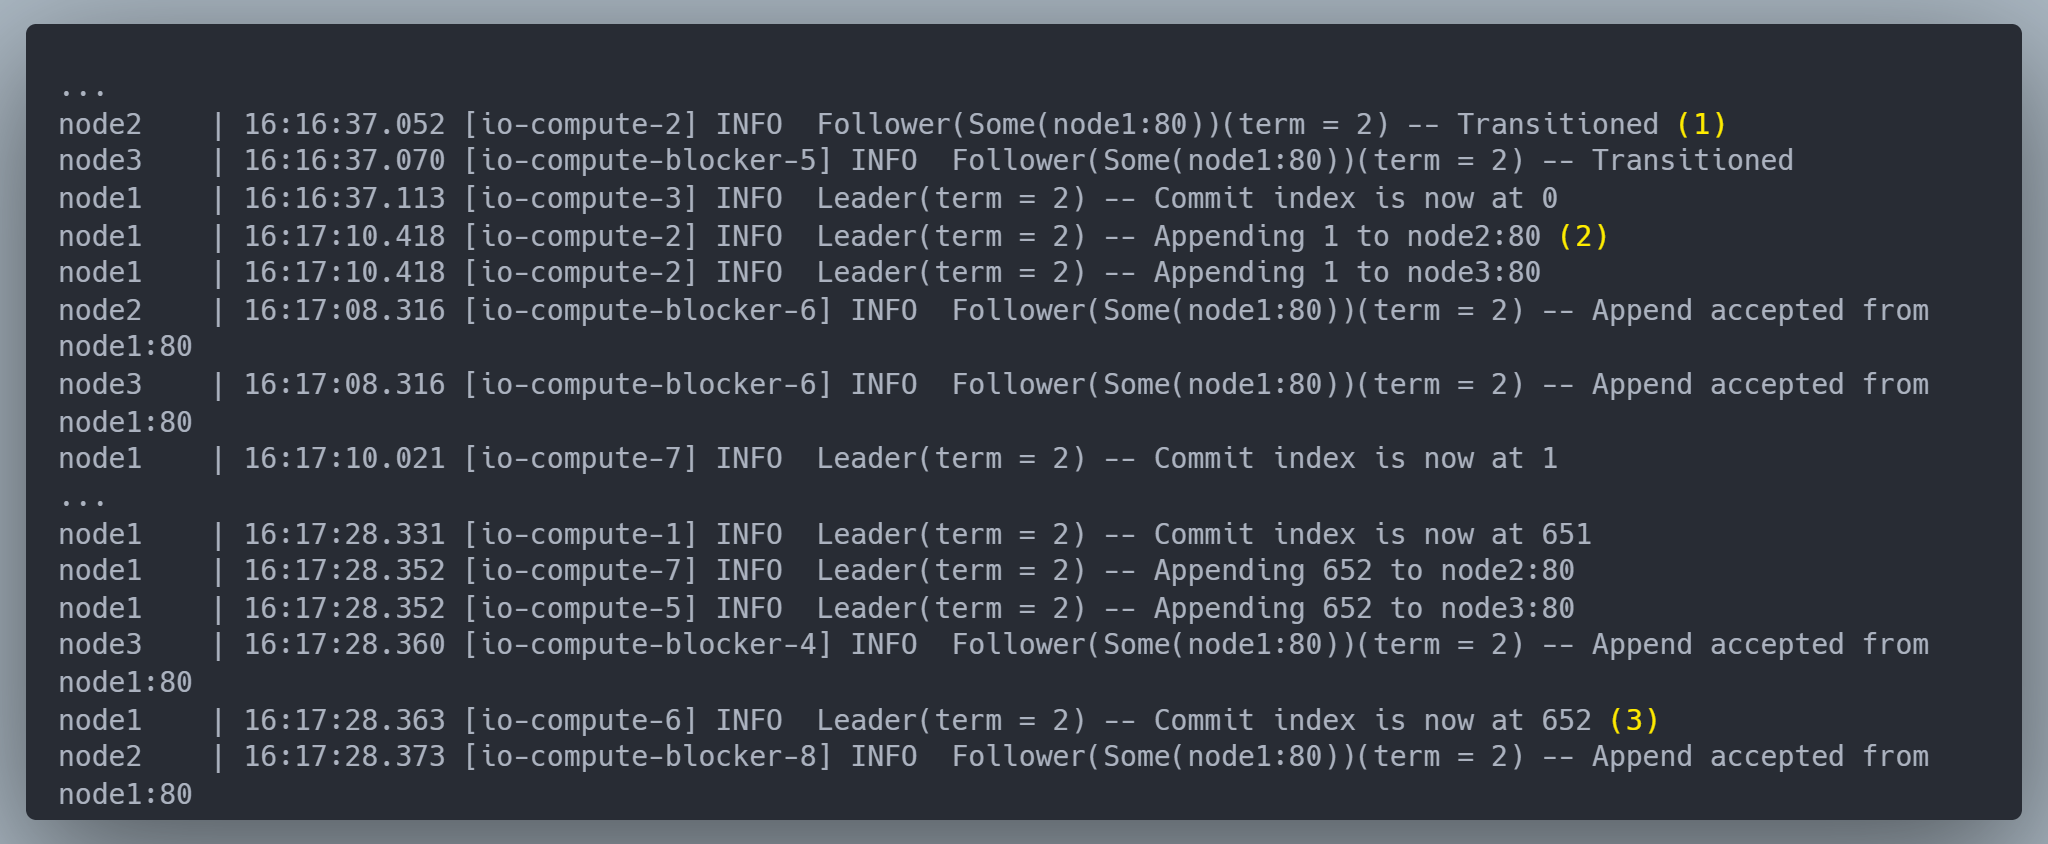
\includegraphics[width=500pt]{images/scenario_8_cluster.png}
\caption{Cluster output for the eighth scenario.}
\label{fig:scenario-8-cluster}
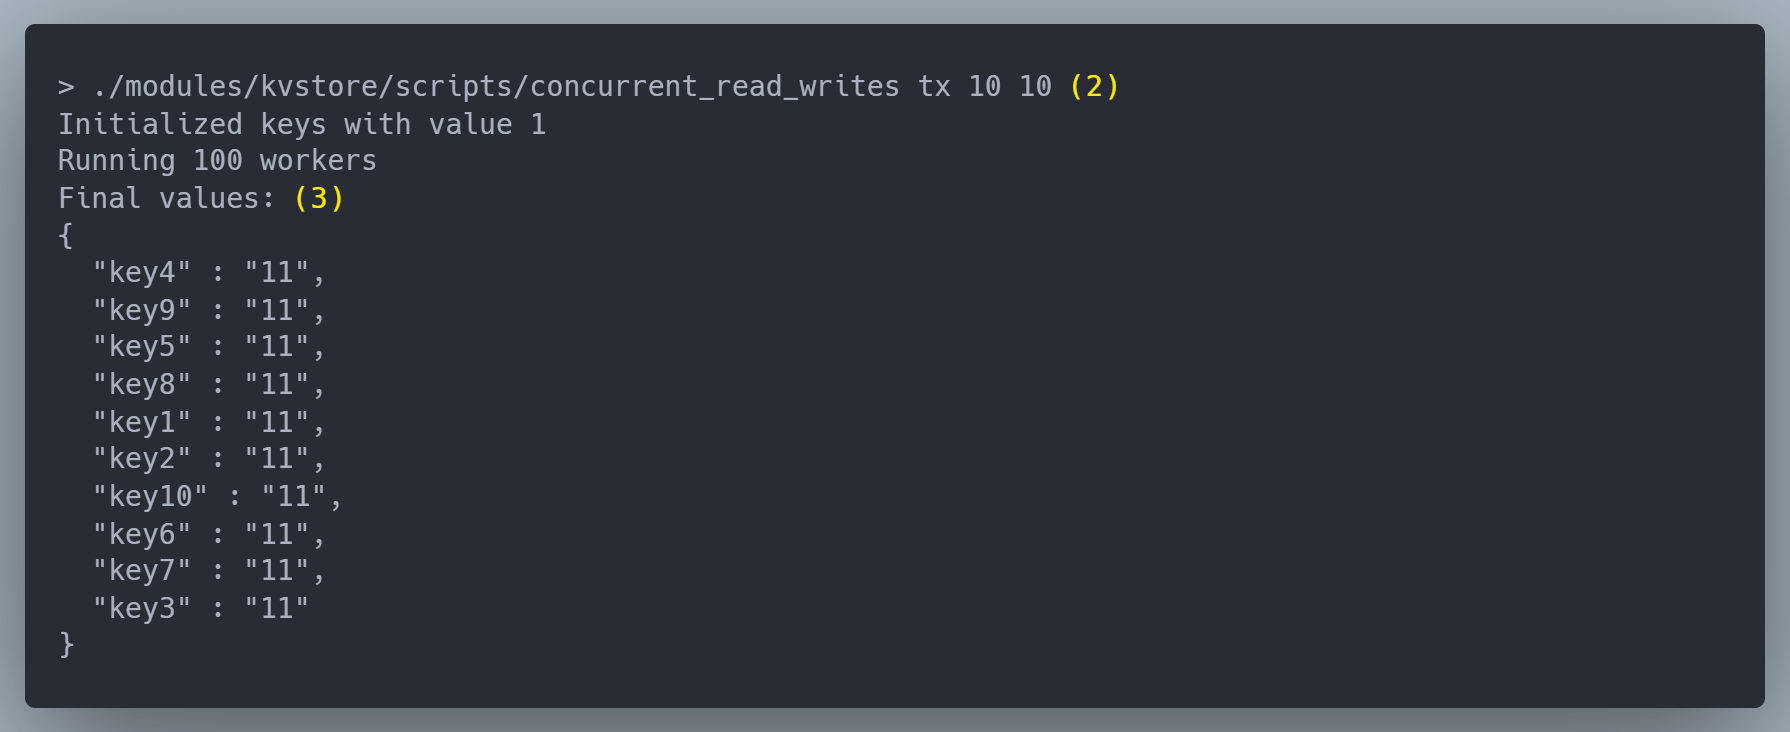
\includegraphics[width=500pt]{images/scenario_8_commands.png}
\caption{Input commands for the eighth scenario.}
\label{fig:scenario-8-commands}
\end{figure}

\subsubsection{Result}
In Figures \ref{fig:scenario-8-cluster} and \ref{fig:scenario-8-commands}, the following events are marked:
\begin{enumerate}
    \item The cluster is stable before any command is issued, with Server 1 being the leader and Servers 2 and 3 being followers.
    \item The script is run externally, which initializes the key-set and then starts up the concurrent workers.
    \item The script ends up generating 652 commands. At that point, the script terminates, showing the final values.
\end{enumerate}

\subsubsection{Commentary}

These results show that it is possible to achieve both concurrency and atomicity when using the implemented transaction mechanism, as all keys correctly reached the expected value of 11.\\

It is also shown that, due to the high contention between the concurrent workers, there were significantly more commands generated than the non-transactional example. With this setup, the theoretical maximum for commands is 652. This is calculated by first taking the commands that were required in the previous scenario, 202, which did not include any retries. Then, the maximum number of retry requests that would have to be sent on each iteration is added. For the first iteration, at worst 9 workers will have to retry for each of the 10 keys, issuing 90 requests. On the second iteration, at worst 8 workers would retry, issuing 80 requests, and so on, so fourth, resulting in the following expression:
\begin{equation}
202 + \sum_{n=1}^{9} ({100-10n}) = 652.
\end{equation}

The theoretical maximum was actually reached with this test setup, since it simulates the worst-case scenario; each iteration is timed so that the most workers possible will have to retry. However, in real-world cases, the number of needed commands would be greatly reduced, as requests would not be purposefully timed to conflict.

\subsection{Issuing Commands to the Cluster Between a Server's Crash and Recovery}

This scenario shows Raft's ability to catch up servers that missed commands due to crashes or other failures.

\subsubsection{Initial State}

The replicated log is empty and the cluster is stable with Server 2 as the leader, as shown under Marker 1 in Figure \ref{fig:scenario-9-cluster}.

\subsubsection{Input}

As shown in Figure \ref{fig:scenario-9-commands}, the \lstinline|docker stop| command is issued to simulate a failure on the leader server. Then, similarly to Scenario \ref{simple-get-put-scenario}, a series of requests is made to the store using \lstinline|curl|. In this case, three \lstinline|PUT| requests are made, each time inserting a unique key-value pair. Finally, the stopped server is restarted.

\begin{figure}[!ht]
\centering
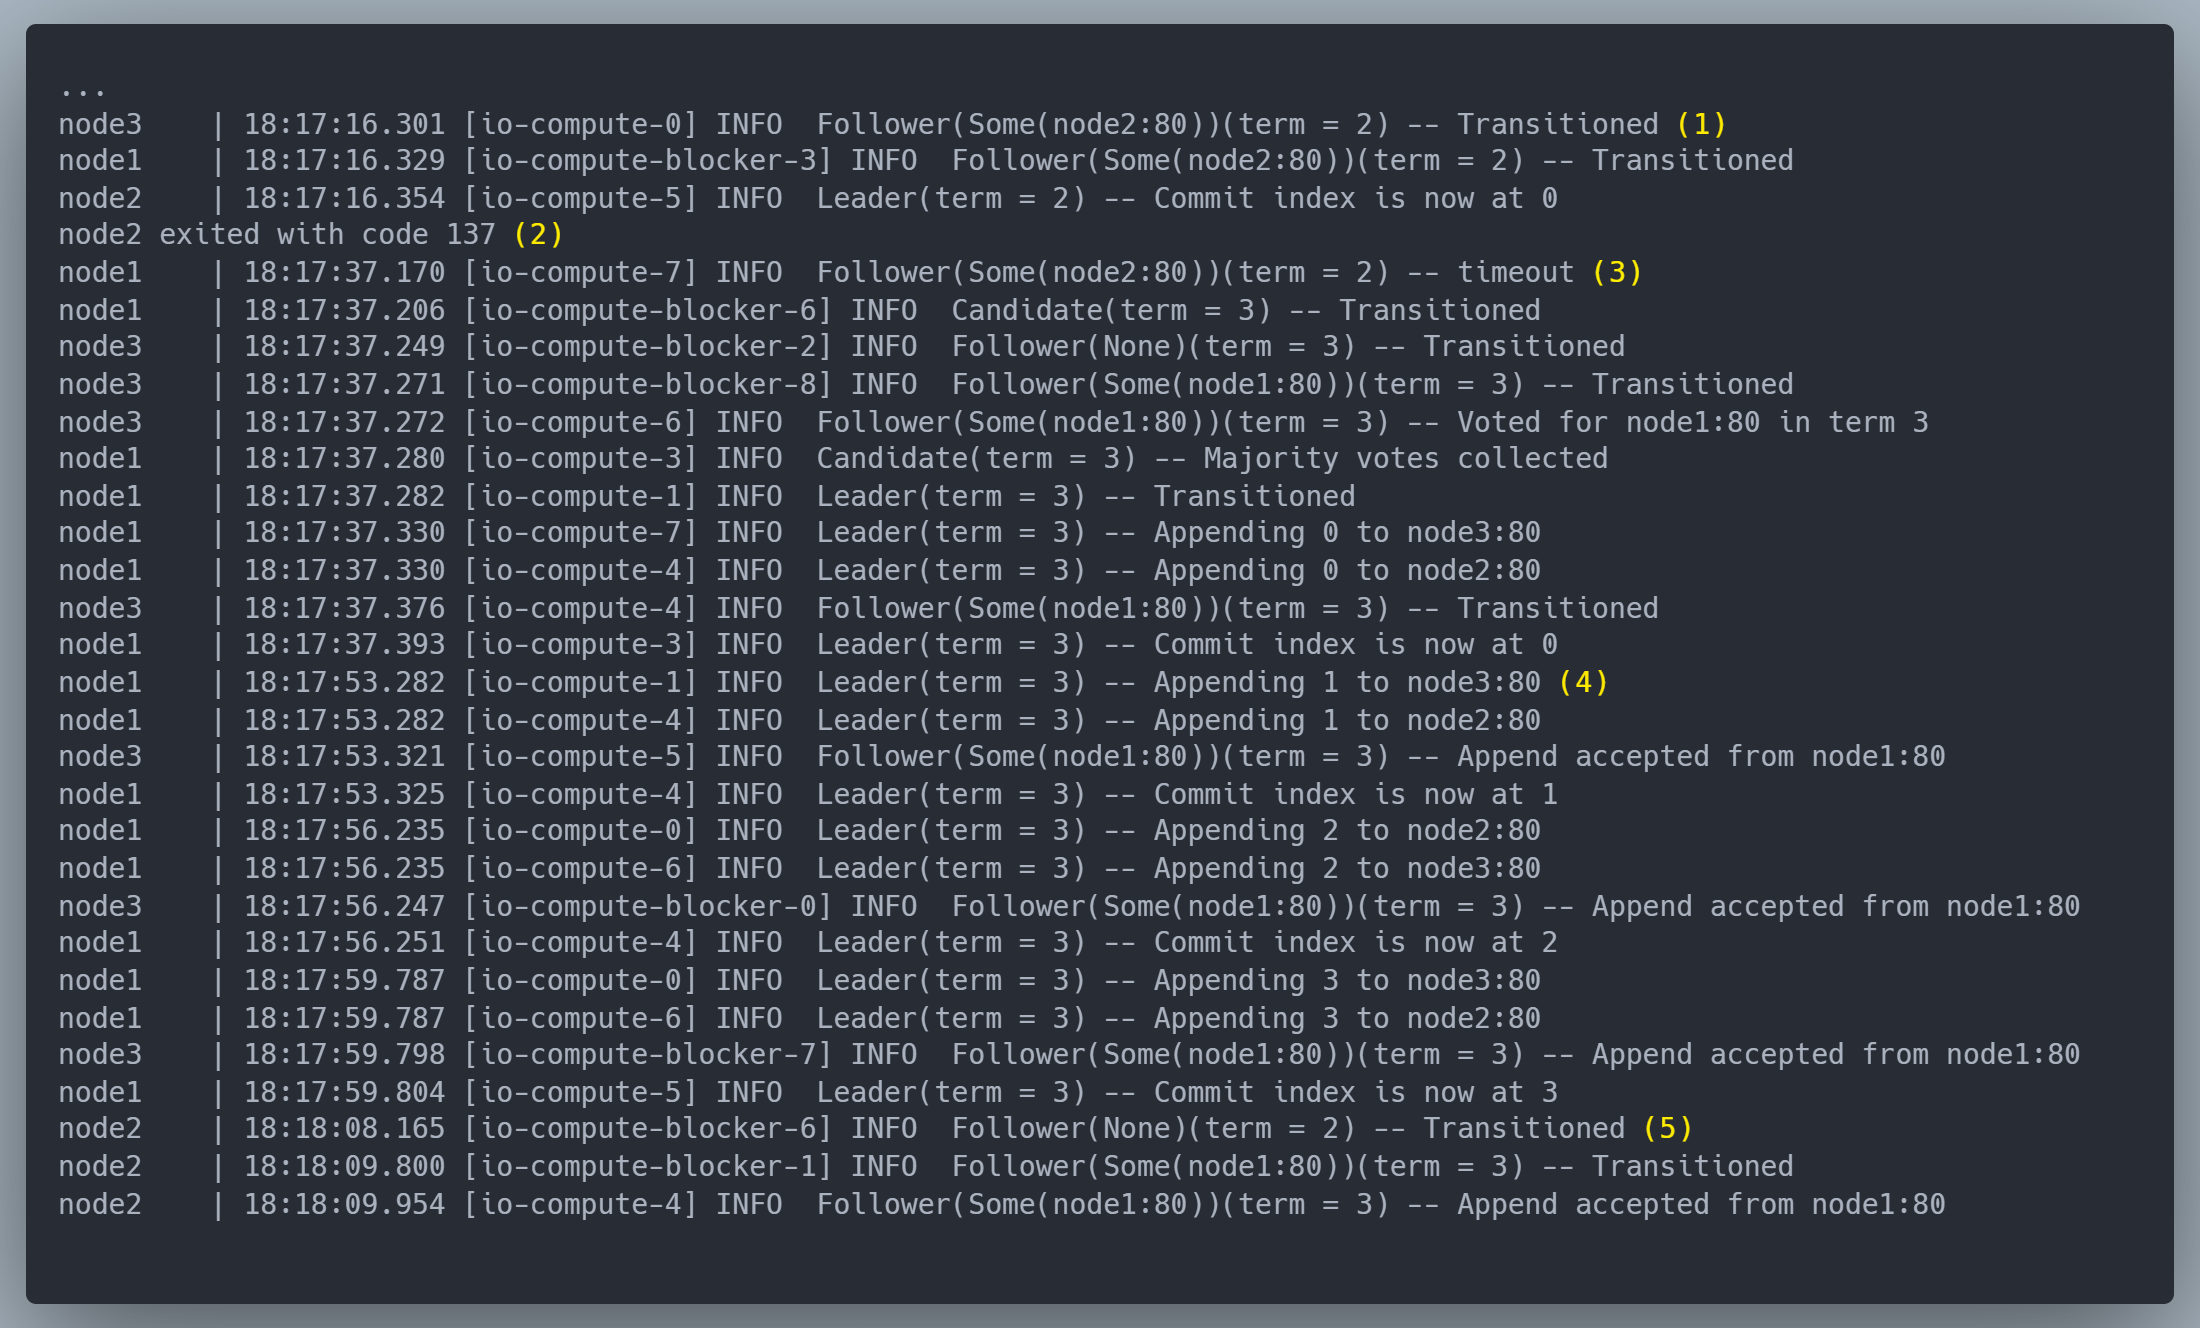
\includegraphics[width=500pt]{images/scenario_9_cluster.png}
\caption{Cluster output for the ninth scenario.}
\label{fig:scenario-9-cluster}
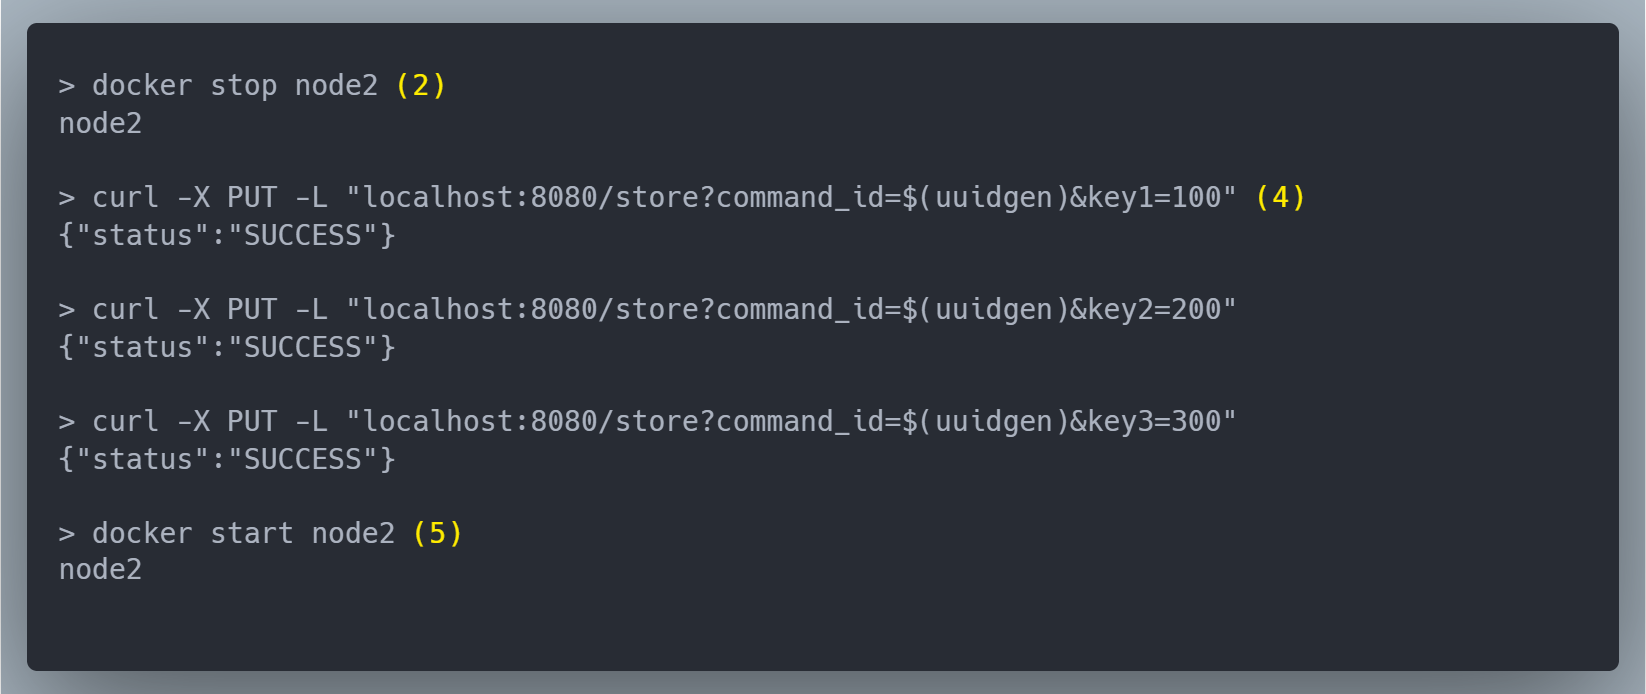
\includegraphics[width=500pt]{images/scenario_9_commands.png}
\caption{Input commands for the ninth scenario.}
\label{fig:scenario-9-commands}
\end{figure}

\begin{figure}[!ht]
\centering
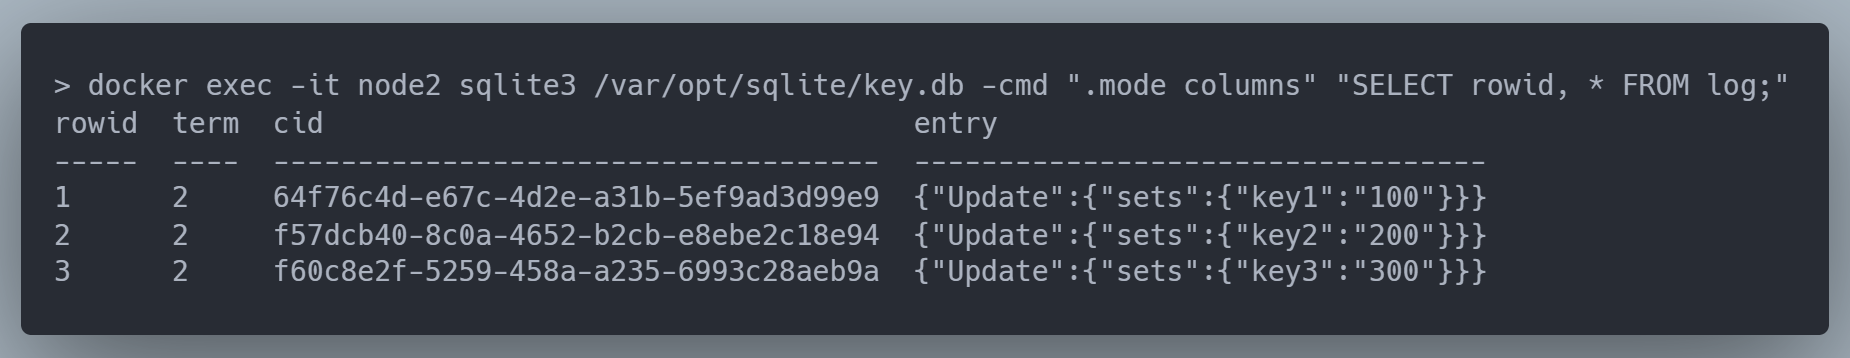
\includegraphics[width=500pt]{images/scenario_9_sqlite.png}
\caption{Input commands for the ninth scenario.}
\label{fig:scenario-9-sqlite}
\end{figure}

\subsubsection{Result}
In Figures \ref{fig:scenario-9-cluster} and \ref{fig:scenario-9-commands}, the following events are marked:
\begin{enumerate}
    \item The cluster is stable before any command is issued, with Server 2 being the leader and Servers 1 and 3 being followers.
    \item Server 2 is stopped via an external command.
    \item The leader election process begins for the next term with Server 1 ending up as the leader.
    \item Three inserts are issued via external commands and are successfully replicated throughout the cluster.
    \item Server 2 is restarted, learns the new term, and receives the log entries it missed. The internal log of Server 2 is now completely up-to-date.
\end{enumerate}

The resulting state of Server 2 can be further demonstrated by examining its local log. This is shown in Figure \ref{fig:scenario-9-sqlite}, where a \lstinline|SELECT| statement is performed against the server's Sqlite log table, using the \lstinline|sqlite3| CLI tool. The output shows the three commands in their internal representation, with all of them having the correct term and index, proving that they were correctly replicated to Server 2 after its recovery.

\subsubsection{Commentary}

These results show that Raft can indeed catch up servers that did not participate in the replication process for a while. Note that, in this scenario, the leader was chosen to be stopped. Had a follower been picked instead, the results would have been almost identical, with one key difference; no leader election process would have been necessary upon the follower's stoppage. 

\subsection{Network Partition Recovery}

This scenario simulates a network partition and demonstrates the store's recovery.

\subsubsection{Initial State}

The replicated log is empty and the cluster is stable with Server 2 as the leader, as shown under Marker 1 in Figure \ref{fig:scenario-10-cluster}.

\subsubsection{Input}

As shown in Figure \ref{fig:scenario-10-commands}, a network partition is simulated by issuing the \lstinline|docker network disconnect| command via the terminal. The partition splits the cluster into two groups; Server 1 and Server 3 are in one group, while Server 2 is in another. The partition is later resolved by using the \lstinline|docker network connect| command.

\begin{figure}[!ht]
\centering
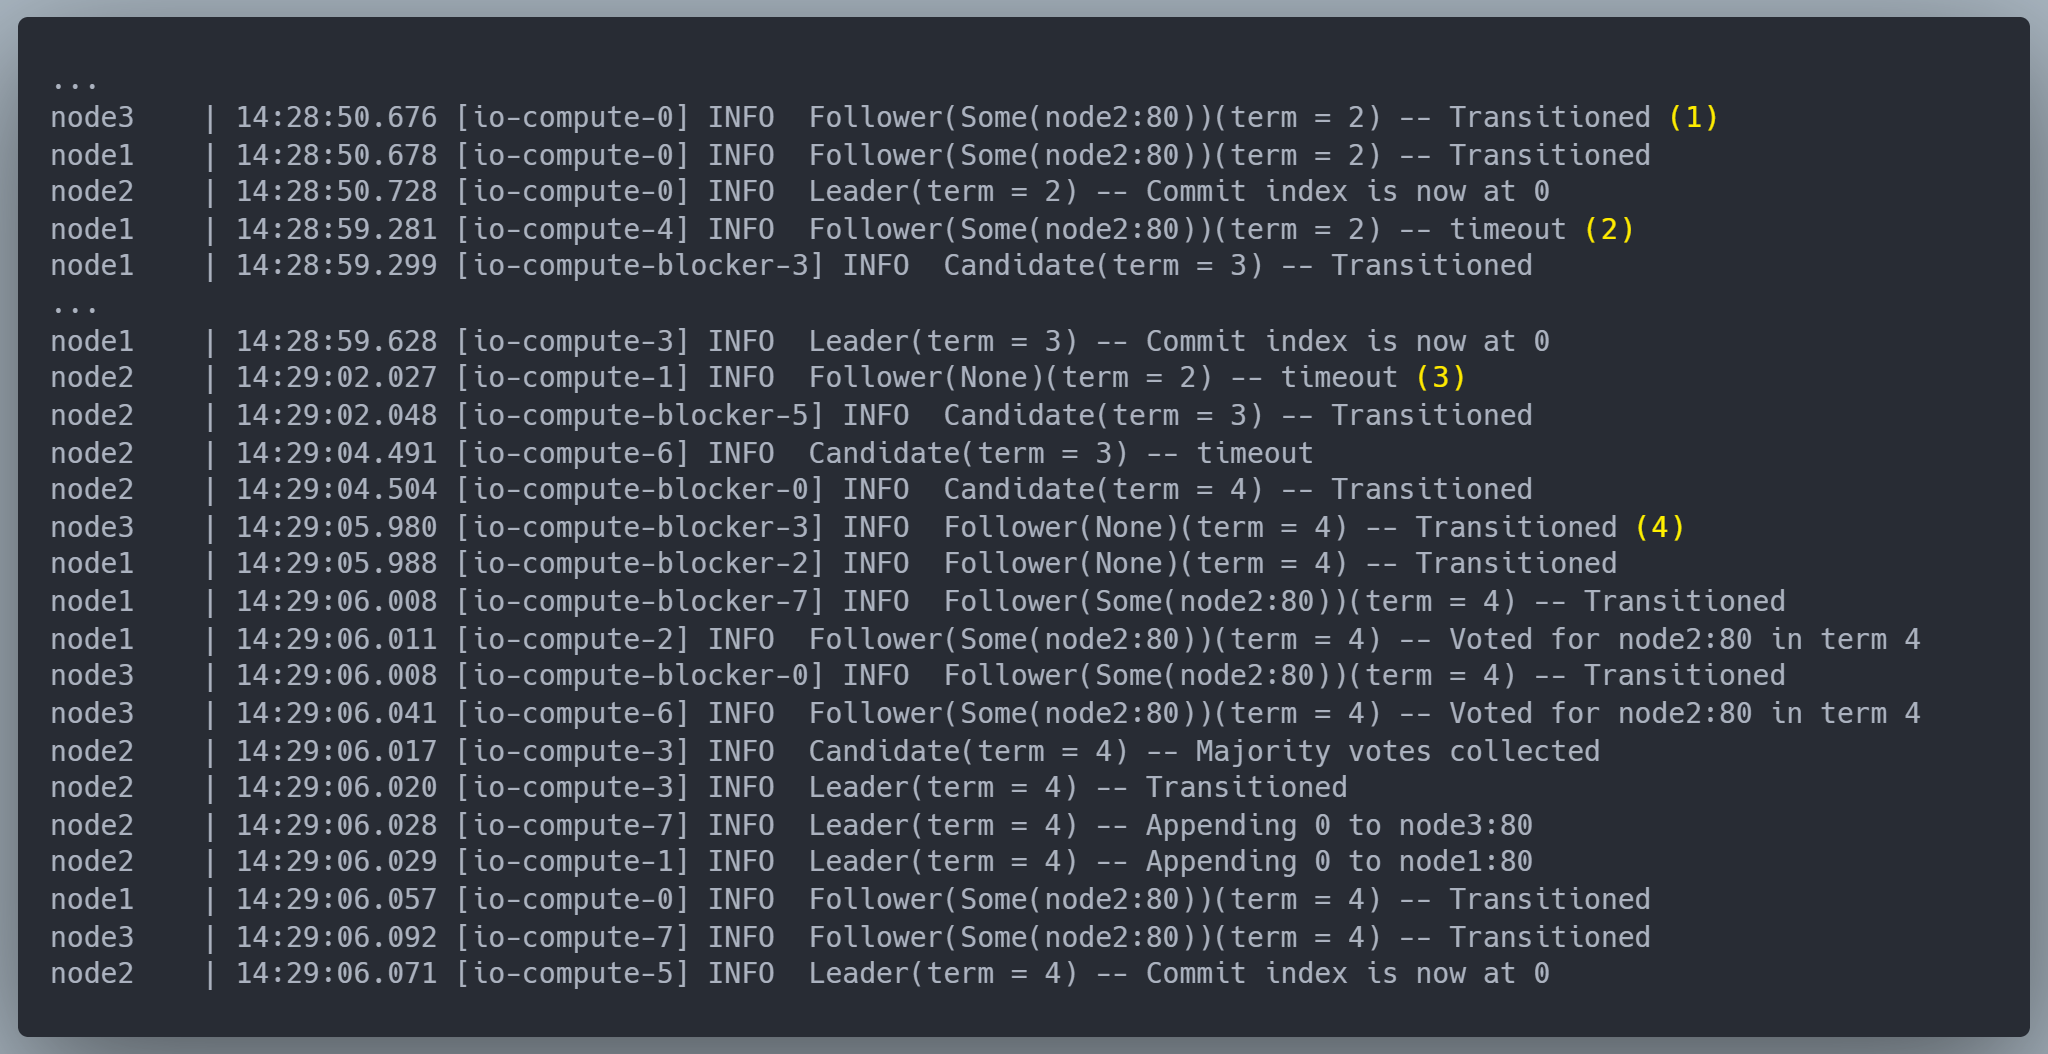
\includegraphics[width=500pt]{images/scenario_10_cluster.png}
\caption{Cluster output for the tenth scenario.}
\label{fig:scenario-10-cluster}
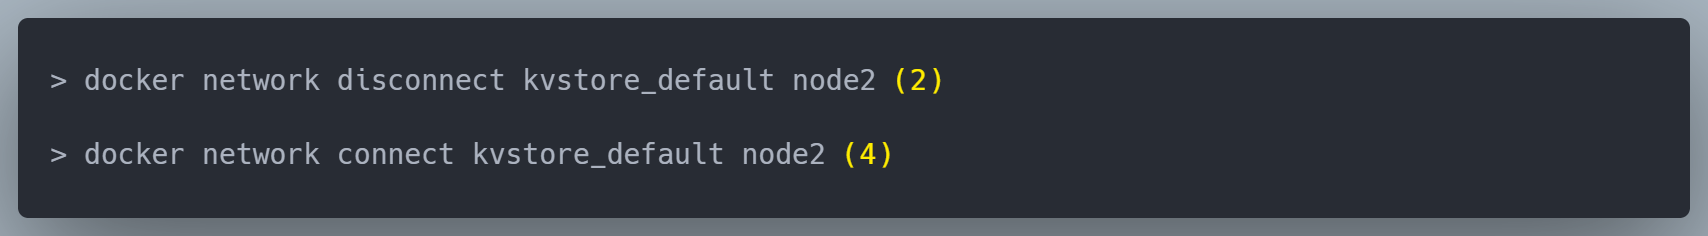
\includegraphics[width=500pt]{images/scenario_10_commands.png}
\caption{Input commands for the tenth scenario.}
\label{fig:scenario-10-commands}
\end{figure}

\subsubsection{Result}
In Figures \ref{fig:scenario-10-cluster} and \ref{fig:scenario-10-commands}, the following events are marked:
\begin{enumerate}
    \item The cluster is stable before any command is issued, with Server 2 being the leader and Servers 1 and 3 being followers.
    \item A network partition is simulated that isolates the leader from its followers. Server 1 detects that there is no viable leader, becomes a candidate for the next term, and wins the election.
    \item Server 2 detects a partition and becomes a follower, since it is unable to reach the other servers. Then, after an election timeout, it becomes a candidate for the next term and attempts to gather votes. Server 2 goes through multiple iterations of unsuccessful election attempts as it remains partitioned.
    \item The partition is resolved and Server 2 can once again reach the other servers. Server 2 then attempts to become the leader again and succeeds. During the election, the other servers adopt the term that Server 2 had reached while partitioned, since its larger than their own terms. 
\end{enumerate}

\subsection{Leader Reelection with Populated Log}

This scenario shows the store's fault tolerance with a populated log.

\subsubsection{Initial State}
The replicated log is empty and the cluster is stable with Server 1 as the leader, as shown under Marker 1 in Figure \ref{fig:scenario-11-cluster}.

\subsubsection{Input}
As shown in Figure \ref{fig:scenario-11-commands}, the log is initially populated by running the \lstinline{concurrent_read_writes} script. This ensures that the log is fairly long and complex. Then, the leader is stopped by issuing a \lstinline{docker stop} command. Finally, the values of the 10 keys created by the \lstinline{concurrent_read_writes} script are requested, using \lstinline{curl}.

\begin{figure}[!ht]
\centering
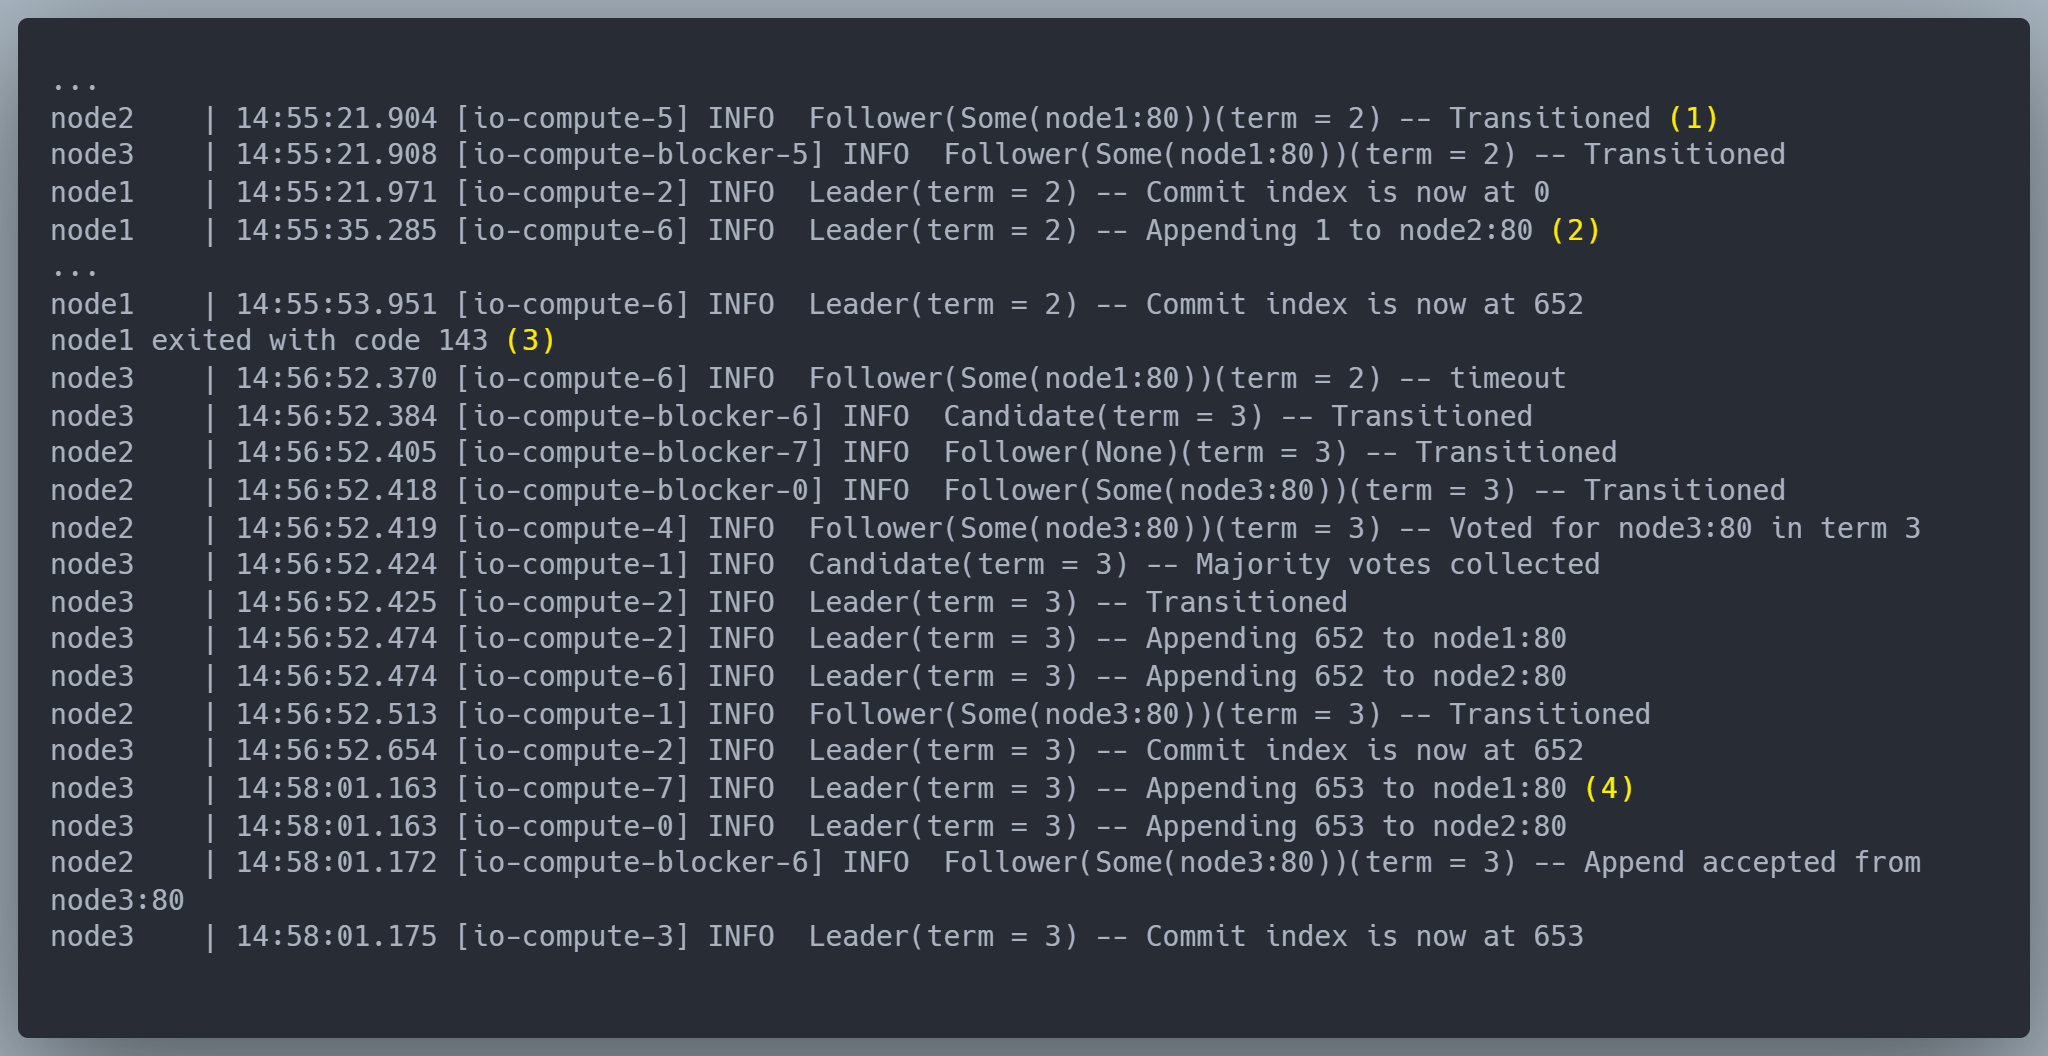
\includegraphics[width=500pt]{images/scenario_11_cluster.png}
\caption{Cluster output for the eleventh scenario.}
\label{fig:scenario-11-cluster}
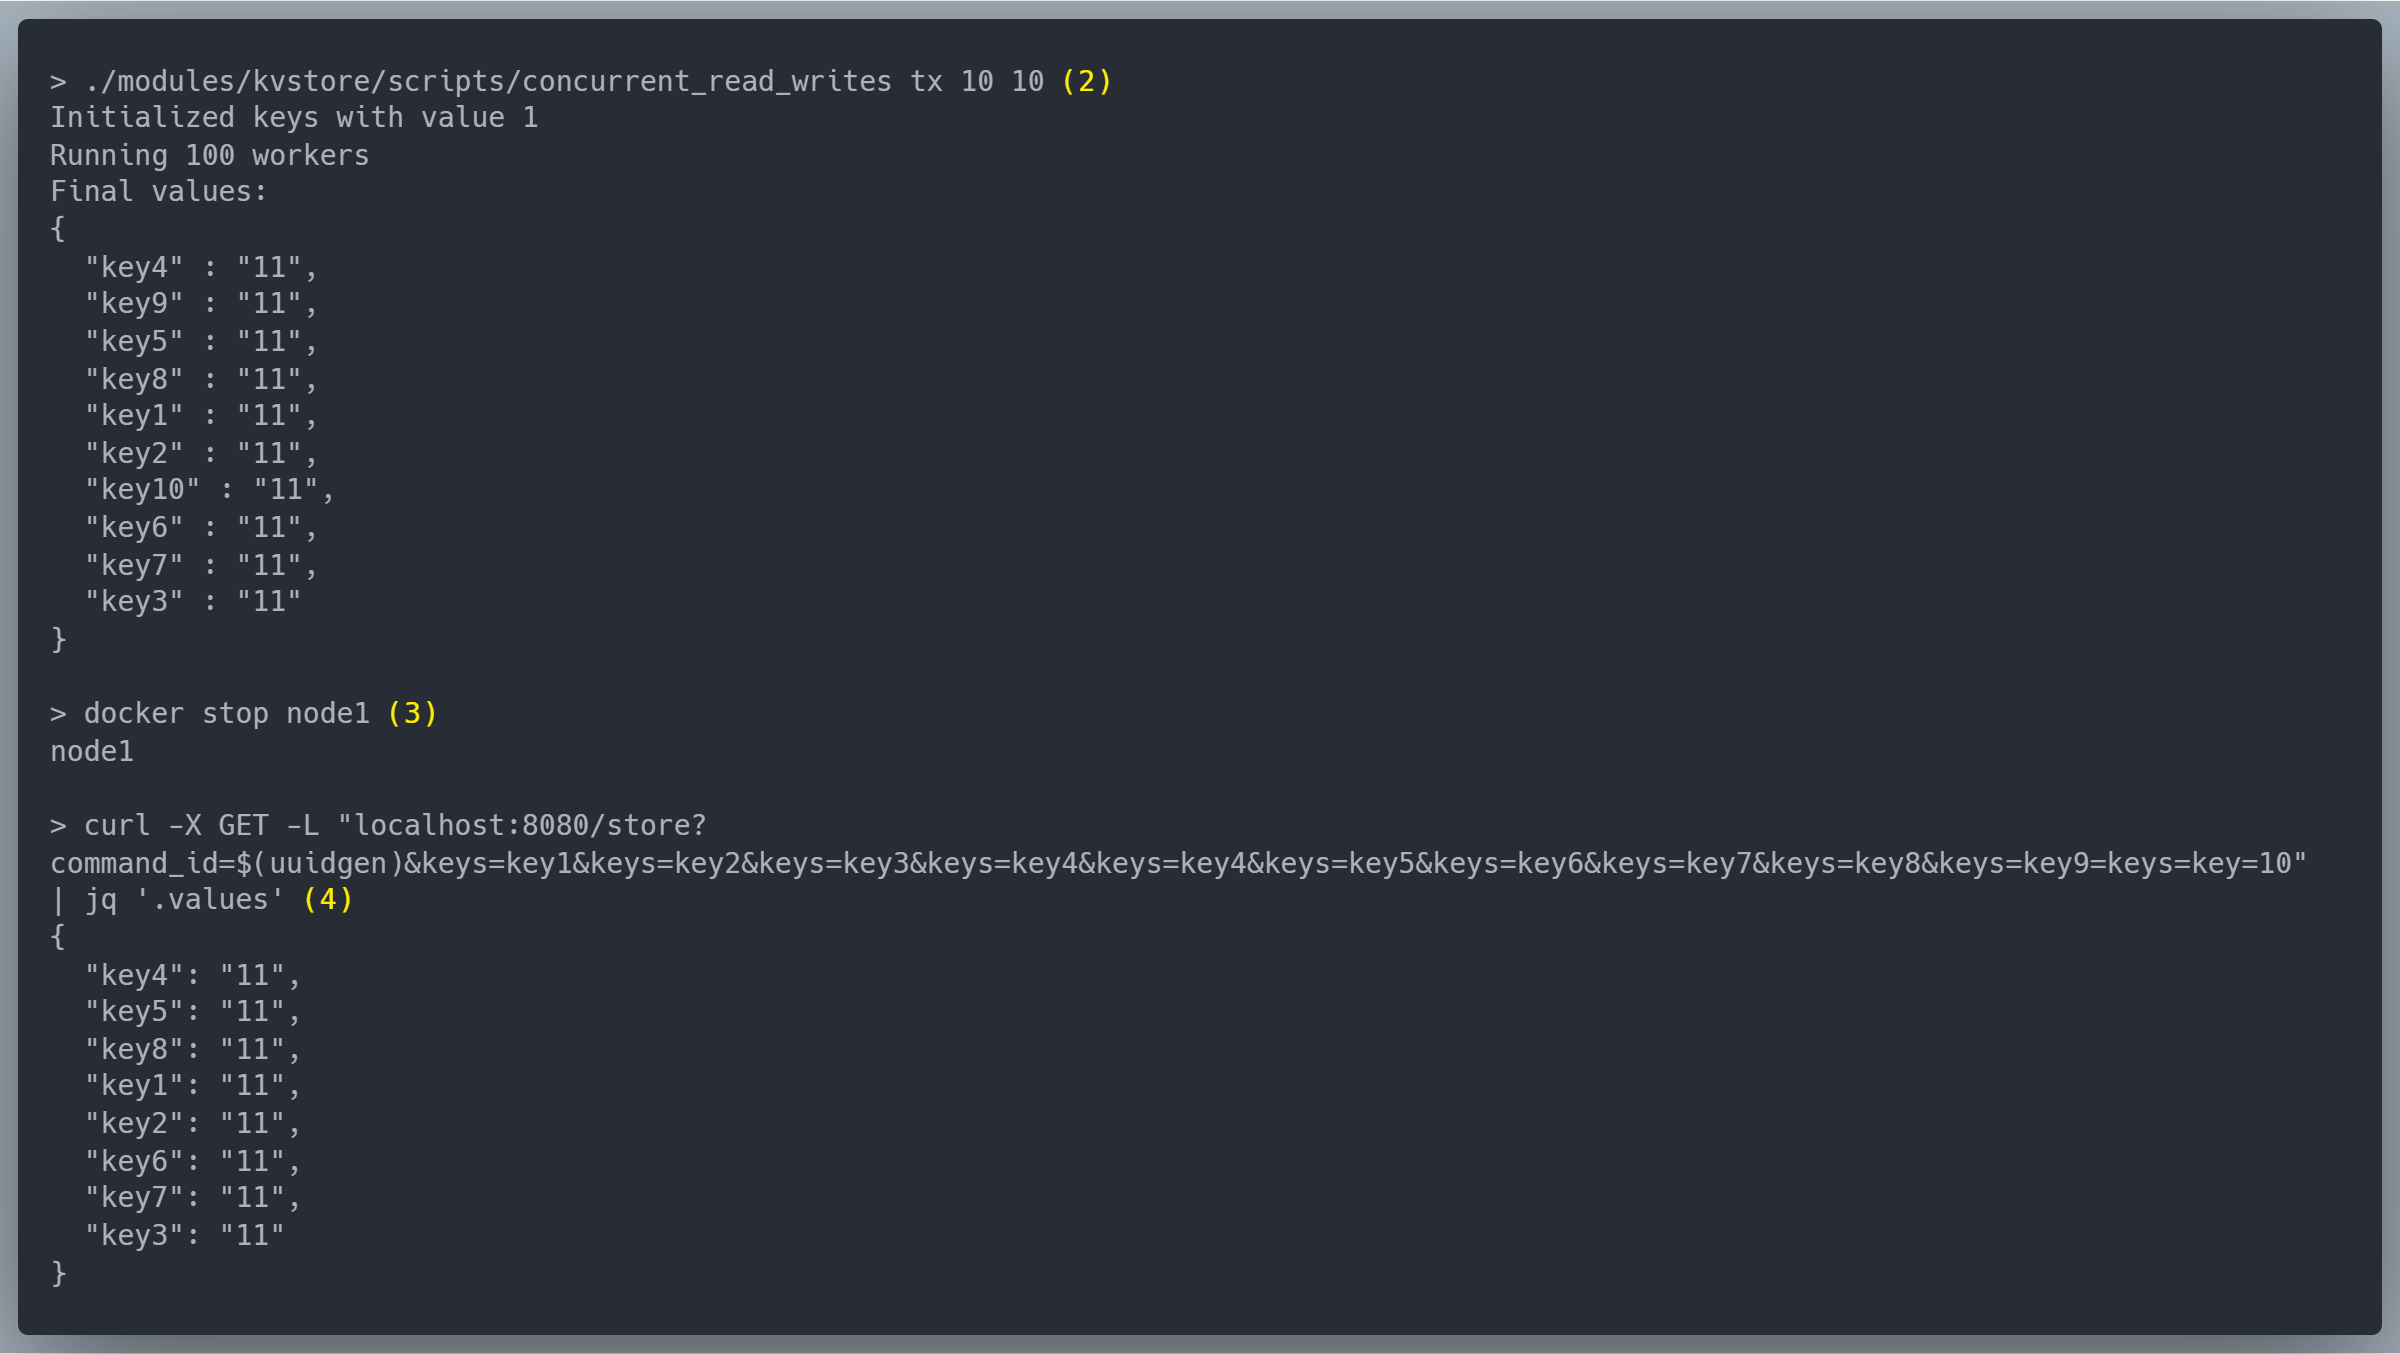
\includegraphics[width=500pt]{images/scenario_11_commands.png}
\caption{Input commands for the eleventh scenario.}
\label{fig:scenario-11-commands}
\end{figure}

\subsubsection{Result}
In Figures \ref{fig:scenario-11-cluster} and \ref{fig:scenario-11-commands}, the following events are marked:
\begin{enumerate}
    \item The cluster is stable before any command is issued, with Server 1 being the leader and Servers 2 and 3 being followers.
    \item The \lstinline{concurrent_read_writes} script is run and the commit index reaches 652.
    \item A crash is simulated in Server 1, which triggers an election, with Server 3 ending up as the new leader.
    \item The values of the keys that were previously inserted are requested. The new leader responds, returning the correct values.
\end{enumerate}

\subsubsection{Commentary}

These results clearly show that the state machine is correctly replicated, enabling the cluster to continue to progress in case of leader failures. Also note that the same would have been true had the leader been partitioned instead of crashing.

\subsection{Command Rejection when Non-Linearizable}

This scenario shows how the store enforces linearizability in the face of duplicate commands. Linearizability is explained in Section \ref{linearizable-semantics}.

\subsubsection{Initial State}
The replicated log is empty and the cluster is stable with Server 3 as the leader, as shown under Marker 1 in Figure \ref{fig:scenario-12-cluster}.

\subsubsection{Input}
Two identical \lstinline|PUT| requests are sent via the terminal with \lstinline|curl|, using the same command id. In addition to the \lstinline|-L| flag that was described in Scenario \ref{L-flag}, the HTTP response codes are shown using the \lstinline|-I| flag. 

\begin{figure}[!ht]
\centering
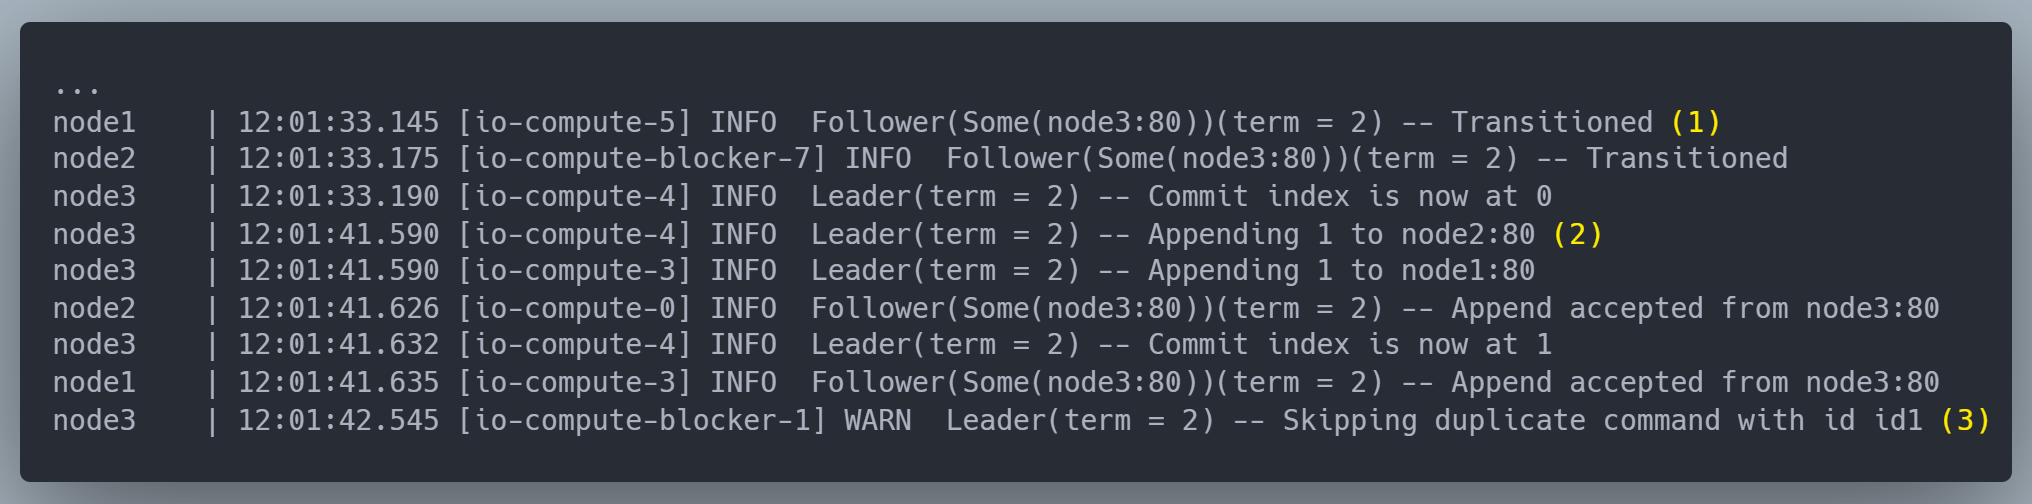
\includegraphics[width=500pt]{images/scenario_12_cluster.png}
\caption{Cluster output for the twelfth scenario.}
\label{fig:scenario-12-cluster}
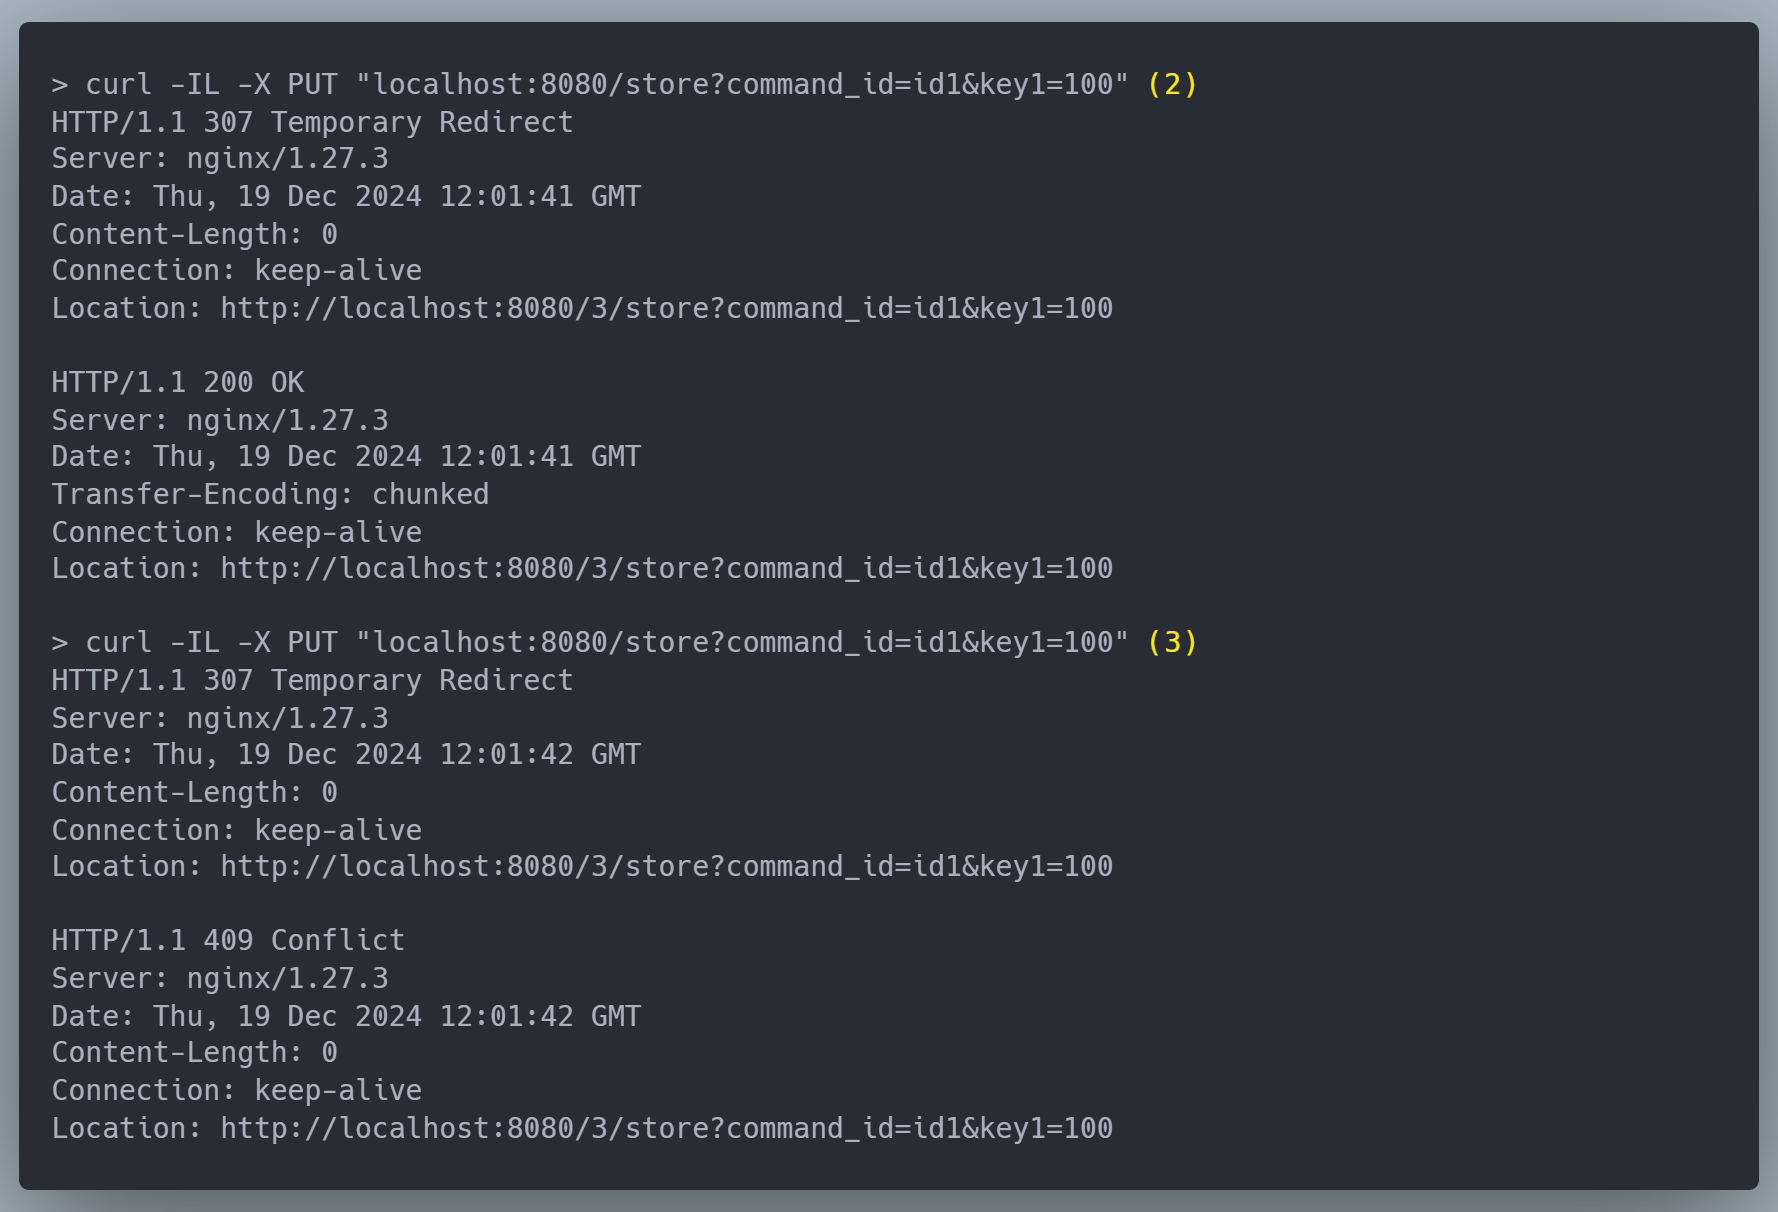
\includegraphics[width=500pt]{images/scenario_12_commands.png}
\caption{Input commands for the twelfth scenario.}
\label{fig:scenario-12-commands}
\end{figure}

\subsubsection{Result}
In Figures \ref{fig:scenario-12-cluster} and \ref{fig:scenario-12-commands}, the following events are marked:
\begin{enumerate}
    \item The cluster is stable before any command is issued, with Server 3 being the leader and Servers 1 and 2 being followers.
    \item The first request is issued via the terminal. The store redirects to the leader server, which accepts the request and commits the command.
    \item The second request is issued, which is rejected after being redirected to the leader. The 409 HTTP code is returned, indicating that the request conflicts with the server's state \cite{409-status-code}.
\end{enumerate}

\chapter{Conclusion and Future Work}

In this chapter, some closing comments are given about this thesis' results and achievements. In addition, a set of ideas for possible follow-up work are presented.

\section{Conclusion}

The main goal of this thesis was to examine Raft and show that it can serve as the backbone for modern, strongly consistent distributed systems. This effort was indeed successful, as Raft, with little modification, was used as the basis for building a distributed key-value store which achieved the desired level of consistency.\\

As shown in the experimental results of this thesis, Raft proved complete for all consensus-related functions of the system, since it performed both leader election and log replication in an adequately fault-tolerant manner. Its implementation was also fairly straight forward and fearless, as its specification is formally proven to be safe \cite{raft}, but also structured in an understandable fashion.\\

Furthermore, this thesis successfully implemented a novel distributed key-value store, serving as a valuable reference for implementing similar systems in the future. The store is also capable enough to be extended in the future and then used directly.

\section{Future Work}

Even though the goals of this thesis were achieved, the resulting system is fairly bare-bones and can be improved in several ways.

\subsection{Missing Common Database Features}

When comparing the implemented system with similar key-value stores, there are several features that are obviously missing.\\

\subsubsection{User Management}

There is absolutely no user management implemented, providing no solution for authentication and access control. This is a feature found in most production-ready databases, as it protects the stored data, but also provides tracing of users' actions.

\subsubsection{Additional Operations}

The implemented system provides the bare minimum set of operations for a key-value store, leaving out features that would make it more convenient in a production environment. At least the following operations should definitely be included in the next version of the system.\\

First, a user cannot select values using some condition when querying; only the selection of keys is allowed. Additionally, the key-selection capabilities of the system are rather poor; a request must contain complete key names and cannot select keys based on a pattern or other conditions. This is not always required, but it is definitely a highly desirable feature for a general-purpose key-value store. Finally, there is no mechanism in place that allows users to dynamically get updates when a key changes value. A user who needs to quickly detect changes has to perform simple reads in a loop instead.

\subsection{Raft Features Not Implemented}

This thesis' implementation of Raft includes all core features that make it a proper consensus mechanism, but lacks some parts of Raft's specification that enable its use in production-ready systems.\\

Raft includes several extensions that make reconfigurations possible without interruption of service. Specifically, Raft includes a process for dynamically adding or removing servers from the cluster. In addition, Raft can enable a leader to voluntarily transfer its authority to another server and revert back to a follower. These features would be necessary for the store's use in real-world deployments, as they enable dynamic scaling of clusters as well as maintenance of servers.\\

Finally, Raft describes a mechanism for compacting the internal logs of servers. The compaction process dramatically reduces the size of the log, saving space and making reads of large log segments more efficient. The latter benefit is particularly important, since reading the entire log is necessary for reconstructing the state machine's current state. As compaction is not implemented in this thesis, reconstructing the state of the key-value store becomes more and more inefficient as the log grows.

\subsection{Alternative Messaging and Persistence Technologies}

As this thesis aimed to present a simple and understandable implementation of a key-value store, the technologies picked for messaging and persistence were simple, but not efficient enough for real-world systems.\\

Regarding server-to-server messaging, HTTP was a straightforward choice, as its semantics match those assumed by the Raft specification. The wide range of tools and libraries supporting HTTP also made the development process quick and enabled easy manual testing. However, in real-world scenarios, there would be a greatly increased volume of messages sent between servers, and the threshold of acceptable latency would be much lower. HTTP would not easily meet these demands, and additional effort should be put into finding and using an alternate technology.\\

Sqlite, the persistence technology used, might also prove inadequate when faced with the log sizes expected in real-world installations of a key-value store. However, this is not as clear cut and should be thoroughly investigated in future efforts.

\subsection{Multi-Raft}

Currently, the store suffers from under-utilizing the follower servers, since they mostly wait passively, serving as live copies of the leader. Additionally, the store cannot comfortably scale to large cluster sizes. These shortcomings are deal-breakers for some data-intensive use-cases and can be addressed by implementing Multi-Raft, as described in Section \ref{scalabilirt-raft-multi-raft}.

\subsection{Intensive Real-World Testing}

Since guesswork can only go so far, a complete list of shortcomings of this thesis' implementation can only be compiled by putting the store through a long-term and thorough test in a production environment. In such an environment, the store should support real services, serving real users. As time goes by, it is expected that the less obvious problems with the current solution would show up and a clear set of required additional features will be presented.

% Bibliography
%\bibliographystyle{ieeetr} % Use IEEE Transactions bibliography style
%\bibliography{includes/references} % Reference list located in 'includes/references.bib'
%% σχόλιο Β
%% Εάν θέλετε να αλλάξετε από biber σε bibtex
%% βγάλτε από τα σχόλια τις πάνω 2 γραμμές και βάλτε σε σχόλιο την παρακάτω
\printbibliography[heading=bibintoc]

% shorthands
\newcommand{\inlineCode}{\lstinline[basicstyle=\normalsize\ttfamily]}

\end{document}
